\documentclass[10pt, oneside, a4paper]{article}   	% {} --> Class: article, report, book, slides
							% [] --> Options: 
							% 11pt = size of the font
							% a4paper, a5paper, letterpaper (default)		
							% titlepage, notitlepage
							% onecolum, twocolumn
							% twoside, oneside = fronteretro o no
							% landscape = foglio orizzontale
								
\usepackage[mode=buildnew]{standalone}
\usepackage[binding=0mm]{layaureo}			% Layout più espanso preimpostato (bindings = spazio rilegatura)
%\usepackage[showframe]{geometry}             		% Layout completamente configurabile
							
\pagestyle{plain}					% plain (default)     :	stampa i numeri di pagine a piè di pagina nel mezzo. 
								%		           
								% headings            :	stampa l'intestazione del capitolo attuale e il numero di pagina 
								%                   		nell'intestazione di ogni pagina, il piè di pagina resta vuoto
								% empty               : stampa nulla
								
%\usepackage{syntonly}					% Per controllare la sintassi senza produrre pagine, risparmio tempo
%\syntaxonly						% QUESTO effettivamente dice al compilatore di non produrre pagine

\usepackage[hidelinks]{hyperref}					% Collegamenti ipertuestuali (link nell'indice)
\usepackage{graphicx}					% Grafica generale
\usepackage{subfig}					% Subfigures
\usepackage{xcolor}					% Per i colori

\usepackage[italian]{babel}				% Regole di a capo, aggiunta di \ap e \ped per apici e pedici in testo
\usepackage[utf8]{inputenc}				% Specifica la codifica
\usepackage{lmodern}					% Evita "sgranatura" font
\usepackage[T1]{fontenc}				% Risolve i problemi di sillabazione 

\usepackage{microtype}					% Migliora il riempimento delle righe
\usepackage{indentfirst}				% Mette un rientro anche alla prima riga dopo il titolo di paragrafo
%\usepackage[parfill]{parskip}    			% Fa cominciare i paragrafi con una riga vuota piuttosto che con un'indentazione

\usepackage{booktabs}					% Linee separatrici per le tabelle
\usepackage[labelfont=bf]{caption}					% Per mettere la didascalia ben distanziata sopra la tabella
\captionsetup[table]{position=bottom}			% 

\usepackage{amsmath}					% Questo lo ha messo dede
\usepackage{float}					% Questo pure, per fissare la posizione di immagini e tabelle

\usepackage{tikz}
\usepackage{adjustbox}
\usepackage{circuitikz}					% Pacchetti per i disegni dei circuiti

\usepackage{amsmath, amsthm, amssymb, amsfonts}		% Matematica

\usepackage{listings}					% Inserimento di codice
\lstset{language=C++}					% Tutti i codici riconosciuti come c++
\lstset{basicstyle=\small\ttfamily,
keywordstyle=\color{blue}\bfseries,
commentstyle=\color{darkgray},
stringstyle=\color{orange}}				% Colori delle righe di codice


\renewcommand{\epsilon}{\varepsilon}			% Varianti lettere greche usate in Europa
\renewcommand{\theta}{\vartheta}			%
\renewcommand{\rho}{\varrho}				%
\renewcommand{\phi}{\varphi}				%
\renewcommand{\d}{\mathrm{d}}
\usepackage{abstract}
\renewcommand{\abstractnamefont}{\normalfont\normalsize\bfseries}
%
%
\begin{document}
\begin{titlepage}
\thispagestyle{empty}
  \begin{center}
    
\includegraphics[width=3.5cm]{img/logo.pdf}%
    %\hspace{0.5cm}%
    %
\includegraphics[width=3.5cm]{img/logodipneg.pdf}
    \\
    \vspace{1cm}
    \Large{Relazione di Laboratorio Avanzato} \\
    \vspace{0.2cm}
    \LARGE{\textbf{DECADIMENTO DEI MUONI\\ COSMICI IN ALLUMINIO}} \\
    \vspace{0.7cm}
    \large
    Mattia Faggin\footnote{[1122479] \texttt{mattia.faggin.1@studenti.unipd.it}},
     Luigi Pertoldi\footnote{[1128283] \texttt{luigi.pertoldi@studenti.unipd.it}}, 
     Davide Piras\footnote{[1114287] \texttt{davide.piras@studenti.unipd.it}} \\
    \vspace{1.8cm}
    \textsl{Università degli Studi di Padova} \\
    \textsl{Dipartimento di Fisica e Astronomia ``Galileo Galilei''} \\
    26 gennaio 2017
%
    \vspace{1cm}
    \begin{abstract}
      \normalsize
      \noindent Lo scopo dell'esperienza di laboratorio è di caratterizzare e ottimizzare un apparato sperimentale per la rivelazione dei muoni cosmici, consistente nei suoi componenti fondamentali di scintillatori plastici e fotomoltiplicatori, e di studiare il loro decadimento in alluminio anche tramite lo sviluppo di modelli analitici e simulazioni Monte Carlo. Vengono infine riportati i valori sperimentali delle costanti di decadimento $\tau^+$ e $\tau^-$ delle rispettive particelle muoniche, nonchè il rapporto numerico tra le due popolazioni $N^+/N^-$.
    \end{abstract}
  \end{center}
  %\vspace*{\fill}
\end{titlepage}
\cleardoublepage
%
\tableofcontents
\clearpage
\listoffigures
\listoftables
%
\clearpage
\section{Introduzione}
L'esperimento si prefigge di registrare il flusso dei muoni cosmici prodotti in atmosfera principalmente dal processo $\pi^+\to\mu^+\nu_\mu$ (e CP coniugato) e studiarne il decadimento in alluminio. All'interno dell'apparato le suddette particelle si comportano in maniera differente in base alla loro carica: i $\mu^+$ decadono unicamente nel canale
\[\mu^+\to e^+\bar{\nu}_\mu\nu_e\ ,\]
mentre i $\mu^-$ possono anche incorrere nel processo di formazione di un atomo mesico, sostituendosi cioè all'elettrone, con una conseguente diminuzione della vita media.

Il flusso dei muoni in funzione dell'angolo azimutale $\theta$ segue una legge del tipo 
\[I(\theta)=I_0\cos^2\theta\ ,\]
con $I_0\sim130\ \text{m}^{-2}\text{s}^{-1}$ a livello del mare \cite{pdg2}.
%
\section{Apparato sperimentale}
La parte dell'apparato adibita alla rivelazione dei raggi cosmici (figura~\ref{appScheme}) consiste di cinque barre (\emph{slab}) di materiale plastico poste parallelamente al terreno ($182 \text{ cm}\times21\text{ cm}\times2.58$ cm), distanti 8 cm tra loro, e altre quattro perpendicolari al terreno poste ai lati ($250\text{ cm}\times21\text{ cm}\times2.58$ cm, riportate solo nello schema laterale) a chiusura dell'apparato. Le \emph{slab} centrali sono accoppiate alle estremità a due fotomoltiplicatori e sono intervallate da spessori di alluminio di 2 cm; quelle laterali fanno invece riferimento a un unico fotomoltiplicatore presente a una sola estremità. Uno strato formato da lastre di piombo per un totale di circa 1 t ricopre infine la parte superiore dell'apparato: il suo scopo è minimizzare la presenza di altre particelle meno energetiche oltre ai muoni e di frenare questi ultimi al fine di osservarne il decadimento.
%
\begin{figure}[H]
	\centering
	\subfloat[Schema frontale.]{
\begin{tikzpicture}
	\newcommand\h{0.1}
	\newcommand\dz{0.2}
	\newcommand\dzA{0.1}
	\newcommand\dzS{\dz+2*\h+\dzA}
	\newcommand\dpmt{0.03}
	
	\node at (-0.3,\dz/2) {4};
	\draw[fill=blue!40!white] (0,0-\dpmt) rectangle (1,\dz+\dpmt);
	\draw[fill=gray!20!white] (1,0) rectangle (2,\dz);
	\draw[fill=gray!40!white] (2,0) rectangle (10,\dz);
	\draw[fill=gray!20!white] (10,0) rectangle (11,\dz);
	\draw[fill=blue!40!white] (11,0-\dpmt) rectangle (12,\dz+\dpmt);
	\node at (12.3,\dz/2) {3};

	\draw[fill=black!80!white] (1.5,\dz+\h) rectangle (10.5,\dz+\h+\dzA);
	
	\node at (-0.3,\dz/2+\dzS) {6};
	\draw[fill=blue!40!white] (0,0+\dzS-\dpmt) rectangle (1,\dz+\dzS+\dpmt);
	\draw[fill=gray!20!white] (1,0+\dzS) rectangle (2,\dz+\dzS);
	\draw[fill=gray!40!white] (2,0+\dzS) rectangle (10,\dz+\dzS);
	\draw[fill=gray!20!white] (10,0+\dzS) rectangle (11,\dz+\dzS);
	\draw[fill=blue!40!white] (11,0+\dzS-\dpmt) rectangle (12,\dz+\dzS+\dpmt);
	\node at (12.3,\dz/2+\dzS) {5};

	\draw[fill=black!80!white] (1.5,\dz+\h+\dzS) rectangle (10.5,\dz+\h+\dzA+\dzS);

	\node at (-0.3,\dz/2+\dzS+\dzS) {8};
	\draw[fill=blue!40!white] (0,0+\dzS+\dzS-\dpmt) rectangle (1,\dz+\dzS+\dzS+\dpmt);
	\draw[fill=gray!20!white] (1,0+\dzS+\dzS) rectangle (2,\dz+\dzS+\dzS);
	\draw[fill=gray!40!white] (2,0+\dzS+\dzS) rectangle (10,\dz+\dzS+\dzS);
	\draw[fill=gray!20!white] (10,0+\dzS+\dzS) rectangle (11,\dz+\dzS+\dzS);
	\draw[fill=blue!40!white] (11,0+\dzS+\dzS-\dpmt) rectangle (12,\dz+\dzS+\dzS+\dpmt);
	\node at (12.3,\dz/2+\dzS+\dzS) {7};

	\draw[fill=black!80!white] (1.5,\dz+\h+\dzS+\dzS) rectangle (10.5,\dz+\h+\dzA+\dzS+\dzS);

	\node at (-0.3,\dz/2+\dzS+\dzS+\dzS) {10};
	\draw[fill=blue!40!white] (0,0+\dzS+\dzS+\dzS-\dpmt) rectangle (1,\dz+\dzS+\dzS+\dzS+\dpmt);
	\draw[fill=gray!20!white] (1,0+\dzS+\dzS+\dzS) rectangle (2,\dz+\dzS+\dzS+\dzS);
	\draw[fill=gray!40!white] (2,0+\dzS+\dzS+\dzS) rectangle (10,\dz+\dzS+\dzS+\dzS);
	\draw[fill=gray!20!white] (10,0+\dzS+\dzS+\dzS) rectangle (11,\dz+\dzS+\dzS+\dzS);
	\draw[fill=blue!40!white] (11,0+\dzS+\dzS+\dzS-\dpmt) rectangle (12,\dz+\dzS+\dzS+\dzS+\dpmt);
	\node at (12.3,\dz/2+\dzS+\dzS+\dzS) {9};

	\draw[fill=black!80!white] (1.5,\dz+\h+\dzS+\dzS+\dzS) rectangle (10.5,\dz+\h+\dzA+\dzS+\dzS+\dzS);

	\node at (-0.3,\dz/2+\dzS+\dzS+\dzS+\dzS) {2};
	\draw[fill=blue!40!white] (0,0+\dzS+\dzS+\dzS+\dzS-\dpmt) rectangle (1,\dz+\dzS+\dzS+\dzS+\dzS+\dpmt);
	\draw[fill=gray!20!white] (1,0+\dzS+\dzS+\dzS+\dzS) rectangle (2,\dz+\dzS+\dzS+\dzS+\dzS);
	\draw[fill=gray!40!white] (2,0+\dzS+\dzS+\dzS+\dzS) rectangle (10,\dz+\dzS+\dzS+\dzS+\dzS);
	\draw[fill=gray!20!white] (10,0+\dzS+\dzS+\dzS+\dzS) rectangle (11,\dz+\dzS+\dzS+\dzS+\dzS);
	\draw[fill=blue!40!white] (11,0+\dzS+\dzS+\dzS+\dzS-\dpmt) rectangle (12,\dz+\dzS+\dzS+\dzS+\dzS+\dpmt);
	\node at (12.3,\dz/2+\dzS+\dzS+\dzS+\dzS) {1};
\end{tikzpicture}}\newline
%
%
\subfloat[Schema laterale.]{
\begin{tikzpicture}
	\newcommand\dz{0.2}
	\newcommand\dl{1.5}
	\newcommand\dD{\dz+0.3}
	\newcommand\dDm{-\dz-0.3}
	\newcommand\dDl{\dz+0.4+\dl}
	
	\draw[fill=gray!40!white] (0,0) rectangle (\dz,\dl);
	\draw[fill=gray!40!white] (0,\dl+0.1) rectangle (\dz, 2*\dl+0.1);
	\draw[fill=blue!40!white] (\dz/2,\dl/2) circle (1.05ex); \node at(\dz/2-0.5,\dl/2) {11};
	\draw[fill=blue!40!white] (\dz/2,\dl/2+\dl+0.1) circle (1.05ex); \node at(\dz/2-0.5,\dl/2+\dl+0.1) {14};

	\draw[fill=gray!40!white] (\dz+0.2,\dl-0.05) rectangle (\dz+0.2+\dl,\dl-0.05+\dz); % slab
	\draw[fill=black!80!white] (\dz+0.2,\dl+\dz+0.1-0.05) rectangle (\dz+0.2+\dl,\dl+\dz+0.1-0.05+\dz/2); %Al
	\draw[fill=blue!40!white] (\dz+0.2+\dl/2,\dl+0.05) circle (1.05ex);

	\draw[fill=gray!40!white] (\dz+0.2,\dl-0.05+\dD) rectangle (\dz+0.2+\dl,\dl-0.05+\dz+\dD);
	\draw[fill=black!80!white] (\dz+0.2,\dl+\dz+0.1-0.05+\dD) rectangle (\dz+0.2+\dl,\dl+\dz+0.1-0.05+\dz/2+\dD);
	\draw[fill=blue!40!white] (\dz+0.2+\dl/2,\dl+0.05+\dD) circle (1.05ex);

	\draw[fill=gray!40!white] (\dz+0.2,\dl-0.05+\dD+\dD) rectangle (\dz+0.2+\dl,\dl-0.05+\dz+\dD+\dD);	
	\draw[fill=black!80!white] (\dz+0.2,\dl+\dz+0.1-0.05+\dDm) rectangle (\dz+0.2+\dl,\dl+\dz+0.1-0.05+\dz/2+\dDm);
	\draw[fill=blue!40!white] (\dz+0.2+\dl/2,\dl+0.05+\dD+\dD) circle (1.05ex); \node at (\dz+0.2+\dl/2,\dl+0.05+\dD+\dD+0.5) {2};

	\draw[fill=gray!40!white] (\dz+0.2,\dl-0.05+\dDm) rectangle (\dz+0.2+\dl,\dl-0.05+\dz+\dDm);
	\draw[fill=black!80!white] (\dz+0.2,\dl+\dz+0.1-0.05+\dDm+\dDm) rectangle (\dz+0.2+\dl,\dl+\dz+0.1-0.05+\dz/2+\dDm+\dDm);
	\draw[fill=blue!40!white] (\dz+0.2+\dl/2,\dl+0.05+\dDm) circle (1.05ex);

	\draw[fill=gray!40!white] (\dz+0.2,\dl-0.05+\dDm+\dDm) rectangle (\dz+0.2+\dl,\dl-0.05+\dz+\dDm+\dDm);
	\draw[fill=blue!40!white] (\dz+0.2+\dl/2,\dl+0.05+\dDm+\dDm) circle (1.05ex); \node at (\dz+0.2+\dl/2,\dl+0.05+\dDm+\dDm-0.5) {4};

	\draw[fill=gray!40!white] (0+\dDl,0) rectangle (\dz+\dDl,\dl);
	\draw[fill=gray!40!white] (0+\dDl,\dl+0.1) rectangle (\dz+\dDl, 2*\dl+0.1);
	\draw[fill=blue!40!white] (\dz/2+\dDl,\dl/2) circle (1.05ex); \node at (\dz/2+\dDl+0.5,\dl/2) {12};
	\draw[fill=blue!40!white] (\dz/2+\dDl,\dl/2+\dl+0.1) circle (1.05ex); \node at (\dz/2+\dDl+0.5,\dl/2+\dl+0.1) {13};
\end{tikzpicture}
%
\hspace{2cm}
%
\begin{tikzpicture}
	\newcommand\dz{0.2}
	\newcommand\dl{1.5}
	\newcommand\dD{\dz+0.3}
	\newcommand\dDm{-\dz-0.3}
	\newcommand\dDl{\dz+0.4+\dl}
	
	\draw[fill=gray!40!white] (0,0) rectangle (\dz,\dl);\node at(\dz/2-0.5,\dl/2) {\textcolor{white}{11}};
	\draw[fill=gray!40!white] (0,\dl+0.1) rectangle (\dz, 2*\dl+0.1);

	\draw[fill=gray!40!white] (\dz+0.2,\dl-0.05) rectangle (\dz+0.2+\dl,\dl-0.05+\dz); % slab
	\draw[fill=black!80!white] (\dz+0.2,\dl+\dz+0.1-0.05) rectangle (\dz+0.2+\dl,\dl+\dz+0.1-0.05+\dz/2); %Al
	\draw[fill=blue!40!white] (\dz+0.2+\dl/2,\dl+0.05) circle (1.05ex); 

	\draw[fill=gray!40!white] (\dz+0.2,\dl-0.05+\dD) rectangle (\dz+0.2+\dl,\dl-0.05+\dz+\dD);
	\draw[fill=black!80!white] (\dz+0.2,\dl+\dz+0.1-0.05+\dD) rectangle (\dz+0.2+\dl,\dl+\dz+0.1-0.05+\dz/2+\dD);
	\draw[fill=blue!40!white] (\dz+0.2+\dl/2,\dl+0.05+\dD) circle (1.05ex);

	\draw[fill=gray!40!white] (\dz+0.2,\dl-0.05+\dD+\dD) rectangle (\dz+0.2+\dl,\dl-0.05+\dz+\dD+\dD);	
	\draw[fill=black!80!white] (\dz+0.2,\dl+\dz+0.1-0.05+\dDm) rectangle (\dz+0.2+\dl,\dl+\dz+0.1-0.05+\dz/2+\dDm);
	\draw[fill=blue!40!white] (\dz+0.2+\dl/2,\dl+0.05+\dD+\dD) circle (1.05ex); \node at (\dz+0.2+\dl/2,\dl+0.05+\dD+\dD+0.5) {1};

	\draw[fill=gray!40!white] (\dz+0.2,\dl-0.05+\dDm) rectangle (\dz+0.2+\dl,\dl-0.05+\dz+\dDm);
	\draw[fill=black!80!white] (\dz+0.2,\dl+\dz+0.1-0.05+\dDm+\dDm) rectangle (\dz+0.2+\dl,\dl+\dz+0.1-0.05+\dz/2+\dDm+\dDm);
	\draw[fill=blue!40!white] (\dz+0.2+\dl/2,\dl+0.05+\dDm) circle (1.05ex);

	\draw[fill=gray!40!white] (\dz+0.2,\dl-0.05+\dDm+\dDm) rectangle (\dz+0.2+\dl,\dl-0.05+\dz+\dDm+\dDm);
	\draw[fill=blue!40!white] (\dz+0.2+\dl/2,\dl+0.05+\dDm+\dDm) circle (1.05ex); \node at (\dz+0.2+\dl/2,\dl+0.05+\dDm+\dDm-0.5) {3};

	\draw[fill=gray!40!white] (0+\dDl,0) rectangle (\dz+\dDl,\dl);\node at (\dz/2+\dDl+0.5,\dl/2) {\textcolor{white}{11}};
	\draw[fill=gray!40!white] (0+\dDl,\dl+0.1) rectangle (\dz+\dDl, 2*\dl+0.1);
\end{tikzpicture}}
	
	\caption{Schema dell'apparato di rivelazione. In nero sono rappresentate le barre di alluminio, i numeri etichettano i vari PMT. Tra le \emph{slab} e i PMT sono presenti delle guide di luce di raccordo.}
	\label{appScheme}
\end{figure}
%
L'alimentazione è regolata da una serie di partitori di tensione che permettono di gestire singolarmente il voltaggio dei 14 fotomoltiplicatori. Essi fanno riferimento ad un unico generatore (impostato ad un valore di circa 2100 V, corrispondente alla massima tensione disponibile per ogni fototubo), acceso sempre qualche ora prima di qualsiasi presa dati e mantenuto costantemente in funzione durante l'acquisizione degli spettri analizzati nel \S\ref{analisireale}.

I segnali provenienti dai PMT, a polarità negativa, di circa 250 mV di ampiezza e 40 ns di larghezza, vengono formati da 14 discriminatori, per poter essere poi inviati agli altri moduli.
%
%
\subsection{Prove di luce - buio}
Il primo controllo eseguito è stato quello relativo alla sensibilità degli scintillatori rispetto alla radiazione ambientale: per ogni fotomotiplicatore si sono raccolti dei conteggi in presenza di luce o in assenza di essa (coprendo l'apparato con teli assorbenti, oscurando le finestre presenti nella stanza e spegnendo le luci) per verificare l'approssimativa indipendenza dell'apparato dalle due condizioni sperimentali. Eventuali infiltrazioni esterne nel rivestimento assorbente delle \emph{slab} sono state riparate con dello scotch isolante nero. 
%
\begin{figure}[h]
	\centering
	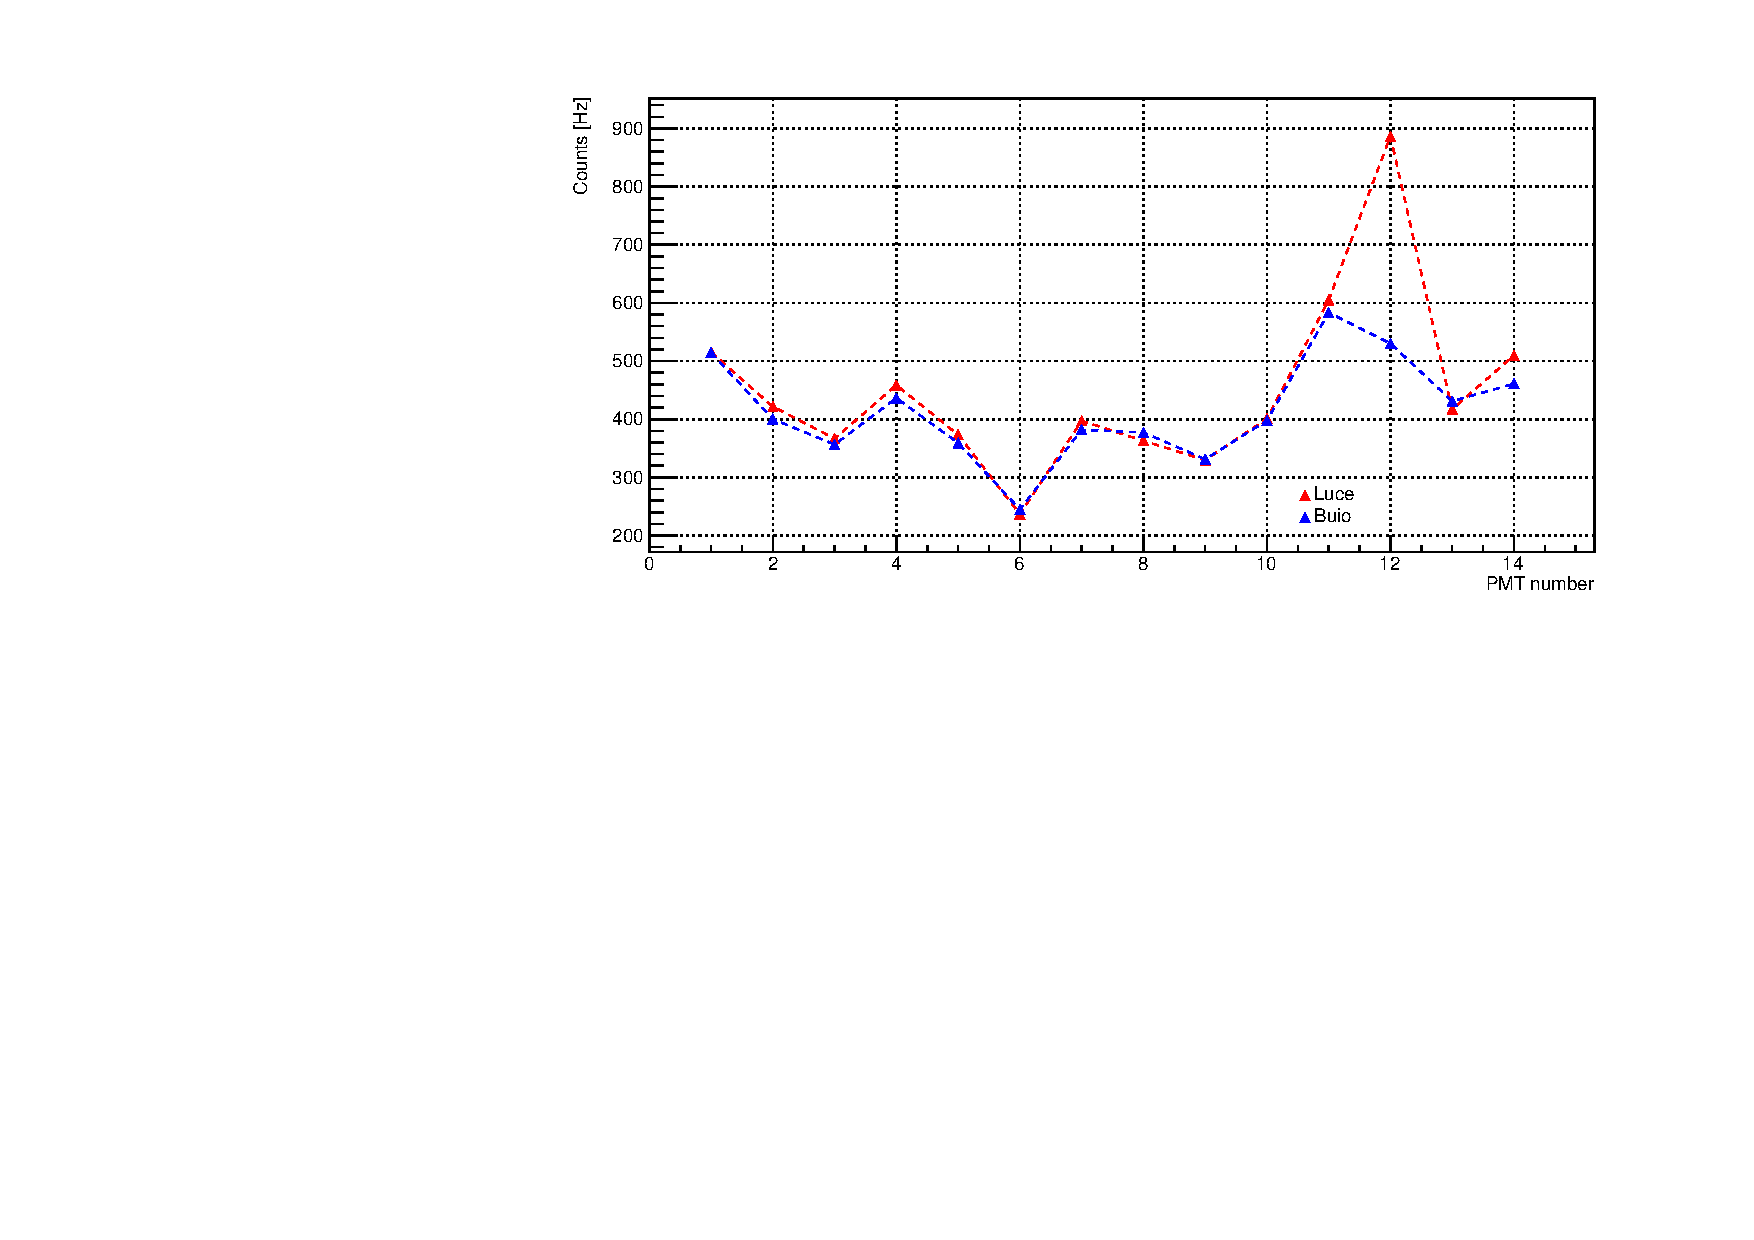
\includegraphics[scale=0.6]{img/luce_buio_100s.pdf}
	\caption{Situazione alla prima presa dati, in blu (rosso) i conteggi al buio (luce): è evidente la presenza di qualche difetto nell'involucro della \emph{slab} a ridosso del fotomoltiplicatore n.~12 che permette l'ingresso della radiazione ambientale.}
\end{figure}
%
\subsection{Studio dell'efficienza dei fotomoltiplicatori}
Lo scopo di questa fase consiste nella determinazione dell'efficienza dei 14 fotomoltiplicatori presenti nell'apparato sperimentale. Il comportamento di un generico fotomoltiplicatore, infatti, dipende dalla tensione a cui è alimentato: al crescere della tensione, l'efficienza di rivelazione aumenta sino a saturare a un valore massimo, raggiungendo dunque il regime di \textit{plateau} rispetto a un contatore di riferimento.
Una volta individuato in quale intervallo di tensioni ciascun fototubo satura, il \emph{set-up} sperimentale ottimale prevede che ciascuno di essi venga alimentato al valore minimo possibile della tensione. 
La condizione di \textit{plateau} è importante per assicurare la massima efficienza di rivelazione possibile; una volta raggiunta, un aumento della tensione di alimentazione coincide solamente con un incremento di rumore.  

L'efficienza di rivelazione corrisponde alla quantità
\[\varepsilon = \frac{T\wedge PMT}{T}\;,\]
dove $T$ corrisponde al numero di eventi rivelati dal cosiddetto \textit{telescopio}, o \textit{trigger}, mentre $T\wedge PMT$ corrisponde alla quantità di eventi rivelati dal fototubo in esame in coincidenza con il telescopio. Il \emph{trigger} prevede l'utilizzo di due \emph{slab} esterne \linebreak ($G$ = grande, $P$ = piccola) poste in coincidenza di volta in volta con alcuni fototubi dell'apparato, differenti da quello momentaneamente esaminato. 

La disposizione del telescopio influenza notevolmente il numero di eventi $T$ tramite i quali si calcola l'efficienza dei diversi fotomoltiplicatori. Ai fini dell'esperimento, l'unica efficienza interessante è relativa alla rivelazione dei raggi cosmici tramite i consueti processi di eccitazione degli atomi del materiale plastico delle \emph{slab}. Tuttavia, questa procedura è stata disturbata dalla presenza delle guide di luce di raccordo tra un capo della \emph{slab} e il relativo fototubo: avendo a disposizione solo due \emph{slab} per formare il telescopio, nel conteggio di trigger entrano, per questioni geometriche, anche quei muoni che attraversano una guida di luce e non le sole \emph{slab}.

In virtù di queste considerazioni, i tracciatori esterni $G$ e $P$ sono stati posizionati sempre parallelamente alle \emph{slab} relative ai PMT esaminati\footnote{$G$ sopra la prima slab, $P$ appoggiata a terra.}: la rivelazione di eventi estranei a quelli di interesse\footnote{Gli eventi di interesse sono quelli relativi a muoni che non attraversano alcuna guida di luce.} non modifica l'andamento della curva di efficienza, ma solamente i valori assunti dalla stessa, permettendo comunque di individuare il raggiungimento del regime di \emph{plateau}.

In base al PMT studiato, il telescopio corrisponde ad una delle seguenti configurazioni:
%%%%%%%%%%%%%%%%%%
\begin{itemize}
	\item[] \textbf{configurazione 1}: per lo studio dei PMT numero 1, 2, 5, 6, 7, 8, 9 e 10 i tracciatori $G$ e $P$ sono messi in coincidenza con i PMT numero 3 e 4 (appartenenti alla \emph{slab} più bassa), cioè \[T = G\wedge P \wedge PMT3 \wedge PMT4 \ ;\]
%
	\item[] \textbf{configurazione 2}: per lo studio dei PMT numero 3 e 4 i tracciatori $G$ e $P$ sono messi in coincidenza con i PMT numero 1, 2, 5, 6, cioè \[T = G\wedge P \wedge PMT1 \wedge PMT2 \wedge PMT5 \wedge PMT6 \ ; \]
%
	\item[] \textbf{configurazione 3}: le \emph{slab} laterali sono state momentaneamente tolte dalla loro posizione originale per essere appoggiate, sovrapposte nella stessa direzione e alternate in verso, su sgabelli di eguale altezza. In questo modo, per lo studio dei PMT 11 e 12, posizionati nello stesso verso, i tracciatori $G$, appoggiato sopra la prima delle quattro \emph{slab}, e $P$, appoggiato a terra, sono stati messi in coincidenza con i PMT numero 13 e 14, anch'essi orientati nello stesso verso, opposto ai precedenti. In questo caso: \[T = G\wedge P \wedge PMT13 \wedge PMT14 \ ;\]
%
	\item[] \textbf{configurazione 4}: questa configurazione coincide con la numero 3, a patto di invertire i ruoli dei PMT 11 e 12 con quelli dei PMT 13 e 14. 
\end{itemize}
%%%%%%%%%%%%%%%%%%%
In appendice B sono riportati i grafici relativi allo studio di tutti i 14 fotomoltiplicatori, sia per quanto riguarda la stima delle efficienze da vicino e da lontano (ovvero con il telescopio posizionato in un punto, sempre lungo la \textit{slab}, più vicino o più lontano possibile rispetto al PMT), sia per quanto riguarda i conteggi da vicino. Si noti che per i PMT 11-14 sono state raccolte solo le curve di efficienza da lontano, per questioni di tempo; inoltre, in qualche grafico sono presenti alcuni punti verdi, che rappresentano alcune misure integrative fatte in un secondo momento.

Al numero di eventi in coincidenza $T\wedge PMT$ è assegnata un'incertezza seguente la distribuzione binomiale, di cui si conosce la formula della varianza.  
Si ha allora che 
\[\sigma_{T\wedge PMT} = \sqrt{T \cdot \varepsilon \cdot  (1-\varepsilon)} \ , \]
dove si è assunta come probabilità dell'evento favorevole il valore sperimentale dell'efficienza $\varepsilon$.
L'errore sull'efficienza è dunque:
$$\sigma_\epsilon=\sqrt{ \left(\frac{\partial\epsilon}{\partial (T\wedge PMT)}\sigma_{T\wedge PMT}\right)^2 + \left(\frac{\partial \epsilon}{\partial T}\sigma_T\right)^2 }=\sqrt{\frac{\epsilon}{T}} \ , $$
dove $\sigma_T = \sqrt{T}$.

%
\subsection{Misure di differenze temporali}\label{tac}
L'acquisizione della curva di decadimento dei muoni necessita di una procedura per la misura di intervalli temporali tramite un modulo Time to Amplitude Converter (TAC) e un modulo Analog to Digital Converter (ADC) per la conversione digitale. Le proprietà desiderate della catena elettronica devono essere opportunamente verificate prima di eseguire una procedura di calibrazione che permetta di associare un canale del multicanale ad un ben preciso valore temporale.
%
\begin{figure}[b!]
  \centering  
  \includestandalone[width=\linewidth]{img/bkg437}
  \caption{Prima analisi dello spettro di ritardi temporali con START e STOP artificiali scorrelati; si nota la presenza di un eccesso di eventi indesiderato nell'intervallo $[2200,2700]$ canali (è stato applicato un \emph{rebin} di un fattore 12 per evidenziare meglio la situazione).}
  \label{rumore1}
\end{figure}
%

Inizialmente si è verificato il corretto comportamento della catena TAC+ADC rispetto a una distribuzione uniforme di ritardi temporali, ovvero generando due treni di segnali artificiali scorrelati da mandare in input alle entrate di START e STOP del TAC; ci si aspetta dalla raccolta di un numero statisticamente rilevante di dati una distribuzione perfettamente piatta. Per l'esperimento si è scelto di utilizzare il TAC n.~437 disponibile in laboratorio: in figura~\ref{rumore1} è possibile osservare i risultati di una prima acquisizione.

Il modulo sembra presentare due problemi: un picco all'inizio dello spettro di cui non si è scoperta l'origine, ma che non influisce sulla raccolta dati, e un eccesso di eventi nell'intervallo $[2200,2700]$ canali (gli stessi problemi sono stati riscontrati con START fisico e STOP artificiale e viceversa, si veda \S\ref{circuito}). Questo secondo problema, di origine anch'essa ignota, rappresenta invece un potenziale fattore di disturbo per l'analisi dati; un possibile approccio alla risoluzione verrà presentato nel \S\ref{analisireale}.

Dopo questa prima fase si è verificato che il TAC non erogasse più di 5 V (il massimo valore di tensione convertibile dall'ADC) in corrispondenza di un ritardo di 20 $\mu$s. Si è proceduto quindi a verificare la linearità della catena elettronica TAC+ADC e a ottenere una calibrazione temporale dello spettro registrato dal multicanale: tramite due copie del segnale di un impulsatore opportunamente discriminato fornite in \textit{input} al TAC, separate da una distanza temporale variabile nell'intervallo $[0 \ \mu \mbox{s},20 \ \mu \mbox{s}]$, si sono registrati i relativi valori di tensione erogati e il canale corrispondente (per i grafici e i valori delle calibrazioni si veda appendice B, figure~\ref{time_tens} e~\ref{chan_time}).

Con il fondoscala impostato come descritto in precedenza, il TAC eroga per valori del ritardo compresi tra 60 ns e 20 $\mu$s segnali nell'intervallo di tensione $[0.211 \ \mbox{V}, 5.070 \ \mbox{V}]$.
%
%
\section{Operazioni preliminari alla presa dati}
\subsection{Conteggi in coincidenza}
La fase di studio successiva consiste nel raccogliere i conteggi in coincidenza tra varie \emph{slab} e, conseguentemente, ottimizzare i valori di tensione applicata ai fotomoltiplicatori al fine di ottenere valori consistenti tra loro e in linea con le previsioni teoriche (si veda in tal proposito l'appendice A). 
Innanzitutto, si sono scelti i valori di tensione dei PMT (riportati in tabella \ref{HV_counts}) 
%
\begin{table}[b]
		\centering
	\begin{tabular}{ccc|ccc}
		\toprule
		PMT	&	HV [V]	&	Frequenza [Hz]	&PMT	&	HV [V]	&	Frequenza [Hz]\\	
		\midrule
		1	&	1860	&	109	&8	&	1890	&	173\\
		2	&	1940	&	91	&9	&	1670	&	128\\
		3	&	1930	&	100	&10	&	1810	&	101\\
		4	&	1920	&	121	&11	&	1750	&	124\\
		5	&	1890	&	121	&12	&	1840	&	82 \\
		6	&	1950	&	105	&13	&	1960	&	86 \\
		7	&	1770	&	123	&14	&	1800	&	197\\
		\bottomrule
	\end{tabular}
%	\begin{tabular}{ccc}
%		\toprule
%		PMT	&	HV [V]	&	Frequenza [Hz]\\	
%		\midrule
%		1	&	1860	&	109	\\
%		2	&	1940	&	91	\\
%		3	&	1930	&	100	\\
%		4	&	1920	&	121	\\
%		5	&	1890	&	121	\\
%		6	&	1950	&	105	\\
%		7	&	1770	&	123	\\
%		8	&	1890	&	173	\\
%		9	&	1670	&	128	\\
%		10	&	1810	&	101	\\
%		11	&	1750	&	124	\\
%		12	&	1840	&	82	\\
%		13	&	1960	&	86	\\
%		14	&	1800	&	197	\\
%		\bottomrule
%	\end{tabular}
	\caption{Tensione finale applicata ai fotomoltiplicatori e relativo numero di conteggi con il piombo posizionato; l'incertezza associata a ciascuna frequenza è di 1 Hz. Le tensioni scelte garantiscono la condizione di \emph{plateau} da distante per ogni fototubo; nel corso dei mesi tali tensioni e frequenze sono state costantemente monitorate.}
	\label{HV_counts}
\end{table}
%
e si sono quindi raccolti i dati di varie coincidenze, prima senza e poi sovrapponendo il piombo, per testare la diminuzione di eventi rivelati in presenza delle lastre, e verificare che il numero di eventi raccolti fosse consistente con quanto atteso dalla geometria dell'apparato (si veda appendice A). I simboli L e R indicano rispettivamente L $= 14 \vee 11 $ e R $= 12 \vee 13$, e insieme alla coppia di PMT 3 e PMT 4 (cioè, S5) formano la cosiddetta \emph{scatola}, utile per i circuiti di START e STOP, analizzati nel paragrafo successivo.
%
\begin{table}[H]
	\centering
	\begin{tabular}{ccc}
		\toprule
		Coincidenze						&	Frequenza senza Pb [Hz] & Frequenza con Pb [Hz]	\\
		\midrule
		S1 (PMT1 $\wedge$ PMT2)					& $60.6 \pm 0.8$	& $52.0 \pm 0.7$ \\
		S2 (PMT9 $\wedge$ PMT10)				& $64.1 \pm 0.8$	& $60.0 \pm 0.8$ \\
		S3 (PMT7 $\wedge$ PMT8)					& $77.2 \pm 0.9$	& $75.1 \pm 0.9$ \\
		S4 (PMT5 $\wedge$ PMT6)					& $63.4 \pm 0.8$	& $61.5 \pm 0.8$ \\
		S5 (PMT3 $\wedge$ PMT4)					& $61.1 \pm 0.8$	& $60.3 \pm 0.8$ \\
		S1 $\wedge$ S2 						& $39.0 \pm 0.6$	& $36.2 \pm 0.6$ \\
		S2 $\wedge$ S3 						& $37.9 \pm 0.6$    	& $36.4 \pm 0.6$ \\
		S3 $\wedge$ S4 						& $37.5 \pm 0.6$	& $36.3 \pm 0.6$ \\
		S4 $\wedge$ S5 						& $36.0 \pm 0.6$	& $35.3 \pm 0.6$ \\
		S1 $\wedge$ S3 						& $29.2 \pm 0.5$	& $26.9 \pm 0.5$ \\
		S1 $\wedge$ S4 						& $22.9 \pm 0.5$	& $21.0 \pm 0.5$ \\
		S1 $\wedge$ S5 						& $17.7 \pm 0.4$	& $16.0 \pm 0.4$ \\
		S1 $\wedge$ S2 $\wedge$ S3				& $29.1 \pm 0.5$	& $27.5 \pm 0.5$ \\
		S2 $\wedge$ S3 $\wedge$ S4				& $28.7 \pm 0.5$	& $27.8 \pm 0.5$ \\
		S3 $\wedge$ S4 $\wedge$ S5				& $28.6 \pm 0.5$	& $27.6 \pm 0.5$ \\
		S1 $\wedge$ S2 $\wedge$ S3 $\wedge$ S4			& $21.8 \pm 0.5$	& $21.8 \pm 0.5$ \\
		S2 $\wedge$ S3 $\wedge$ S4 $\wedge$ S5			& $20.8 \pm 0.5$	& $21.0 \pm 0.5$ \\
		S1 $\wedge$ S2 $\wedge$ S3 $\wedge$ S4 $\wedge$ S5	& $16.7 \pm 0.4$	& $16.7 \pm 0.4$ \\	
		S1 $\wedge$ S2 $\wedge$ L				& $8.9 \pm 0.3$		& $8.8 \pm 0.3$	\\
		S1 $\wedge$ S2 $\wedge$ R				& $8.4 \pm 0.3$		& $7.7 \pm 0.3$	\\
		S3 $\wedge$ S4 $\wedge$ L				& $7.5 \pm 0.3$		& $8.0 \pm 0.3$	\\
		S3 $\wedge$ S4 $\wedge$ R				& $9.2 \pm 0.3$ 	& $9.3 \pm 0.3$	\\
		S1 $\wedge \ (\overline{\mbox{S5}\vee \mbox{L} \vee \mbox{R}})$ (veto)	& $51.3 \pm 0.7$	& $43.2 \pm 0.7$	\\
		\bottomrule
	\end{tabular}
	\caption{Coincidenze. 
	Si noti che nell'ultima misura si è utilizzato il veto per negare il segnale, in quanto esso è risultato più efficiente dell'uscita negata dei discriminatori nell'individuare il segnale voluto: talvolta, infatti, l'uscita negata dei discriminatori non forniva in uscita il segnale desiderato, probabilmente a causa di un malfunzionamento dei moduli o di un problema nella temporizzazione dei segnali. Per ovviare a ciò, con riferimento all'ultima coincidenza, si è messo il segnale S5 $\vee$ L $\vee$ R (opportunamente temporizzato) nell'ingresso di veto del discriminatore del segnale S1: qualora il veto sia attivo, l'\textit{output} risulta nullo.}
	\label{coincidenze}
\end{table}
%
\subsection{Costruzione del circuito}\label{circuito}
A questo punto, dopo tutte le verifiche necessarie, e dopo aver ripetuto le prove di luce-buio\footnote{Si è notato un eccesso di segnale proveniente da una zona della \emph{slab} superiore, subito risolto con del nastro isolante.}, si sono costruiti i circuiti di START e di STOP per la rivelazione dei muoni cosmici. Si rende necessario fare una premessa: potendo utilizzare nella costruzione del circuito segnali negati o di veto, dopo alcune prove si è optato per la seconda possibilità, avendo cura di temporizzare bene le coincidenze, ossia facendo in modo che il segnale di veto, se presente, rendesse effettivamente cieco l'apparato. In questo passaggio il segnale di veto è stato ritardato e allargato cosicchè contenesse il segnale dei PMT in coincidenza.

Per il segnale di START, corrispondente al muone che entra dall'alto e non esce dalla scatola, si è partiti considerando varie possibilità; il miglior compromesso, che generasse un segnale sufficientemente privo di rumore ma con una frequenza di conteggio non troppo bassa, si è rivelato essere il segnale S1 $\wedge$ S2  $\wedge$ $\overline{\mbox{S5}\vee \mbox{L} \vee \mbox{R}}$ , la cui frequenza in coincidenza è 6.6 Hz.
Il segnale di STOP corrisponde invece all'avvenuto decadimento e rivelazione dell'elettrone emesso, ed è stato scelto essere (S3 $\veebar$ S4)  $\wedge$ $\overline{\mbox{S1} \vee \mbox{S5}\vee \mbox{L} \vee \mbox{R}}$, con frequenza 38.1 Hz (schemi in figura~\ref{scemi}).

A questo punto, con i segnali START e STOP fisici si sono ripetuti i test di uniformità descritti alla sezione~\ref{tac}, utilizzando START artificiale con STOP fisico e viceversa: si riscontra lo stesso eccesso di eventi attorno al canale 2500 individuato durante la caratterizzazione del TAC.
%
\begin{figure}[h]
	\centering
	 \subfloat[START.]
 {\begin{circuitikz}
      \draw 
      (0.5,10.97)  to[short,o-] (1.5,10.97)
      (0.5,11.53)  to[short, o-] (1.5,11.53)
      (2.88,11.25) node[american and port] {}
		   node[left=6pt] {\tiny{AND}}
      (0.5,10.97) node[below] {S2}
      (0.5,11.53) node[above] {S1}
      (3.03,11.25) to [short,-o] (5.3, 11.25)
      (2.5,6.97)  to[short,o-] (3.5,6.97)
      (2.3,7.25)  to[short,o-] (3.93,7.25)
      (2.5,7.53)  to[short, o-] (3.5,7.53)
      (2.5,6.97) node[below] {L}
      (2.5,7.53) node[above] {R}
      (2,7.25) node[] {S5}     
      (4.88,7.25) node[american or port] {}
                  node[left=6pt] {\tiny{OR}}
      (5.03,7.25) to[short] (5.03, 11.25)
      (4.85, 10.60) node[rotate=90] {\scriptsize{VETO}}
      ;
    \end{circuitikz}}
    \hspace{1.5 cm}
\subfloat[STOP.]
{\begin{circuitikz}
      \draw 
      (0.5,10.97)  to[short,o-] (1.5,10.97)
      (0.5,11.53)  to[short, o-] (1.5,11.53)
      (2.88,11.25) node[american or port] {}
		   node[left=6pt] {\tiny{OR}}
      (3.4,9.15) node[american and port] {}
		 node[left=6pt] {\tiny{AND}}
      (1, 8.87) to[short] (1, 10.97)
      (1, 8.87) to[short] (2.03, 8.87)
      (1.3, 9.43) to[short] (1.3, 11.53)
      (1.3, 9.43) to[short] (2.03, 9.43)
      (3.55, 9.15) to[short] (4.2, 9.15)
      (4.2, 9.15) to[short] (4.2,7.73)
      (0.5,10.97) node[below] {S4}
      (0.5,11.53) node[above] {S3}
      (3.03,11.25) to [short,-o] (5.3, 11.25)
      (2.5,6.97)  to[short,o-] (3.5,6.97)
      (2.3,7.15)  to[short,o-] (3.93,7.15)
      (2.3,7.35)  to[short,o-] (3.93,7.35)
      (2.5,7.53)  to[short, o-] (3.5,7.53)
      (2.5,6.97) node[below] {L}
      (2.5,7.53) node[above] {R}
      (1.9,7.07) node[] {S1}     
      (1.9,7.43) node[] {S5}   
      (4.88,7.25) node[american or port] {}
		  node[left=6pt] {\tiny{OR}}
      (5.03,7.25) to[short] (5.03, 11.25)
      (4.85, 10.60) node[rotate=90] {\scriptsize{VETO}}
           ;
    \end{circuitikz}}

	\caption{Schema dei circuiti di START e di STOP. Si noti che nel circuito di STOP si è utilizzato un segnale di XOR, ossia il veto ha una componente che rende cieco l'apparato quando entrambe le \emph{slab} S3 e S4 rivelano un evento; ciò viene utilizzato per cercare di incrementare la probabilità che il segnale di STOP non sia dato da un evento spurio, assumendo che una volta decaduto il muone l'elettrone venga rivelato dalla slab successiva e poi si fermi.}
	\label{scemi}
\end{figure}
%
\section{Analisi dati preliminare}\label{analPrelim}
Dopo aver impostato il circuito come illustrato precedentemente, si è proceduto all'acquisizione dei dati relativi al ritardo che intercorre tra il passaggio del muone rivelato dallo START e l'uscita dell'elettrone di decadimento rivelato dallo STOP.

I dati consistono di tre acquisizioni, per un totale di circa 75000 eventi, riguardanti due popolazioni differenti di muoni:
\begin{itemize}
  \item i $\mu^+$, tali che $\mbox{Br}(\mu^+ \to e^+\nu_e\overline{\nu}_\mu)\simeq 100 \%$ e aventi una vita media \linebreak $\tau^+=(2.1969811 \pm 0.0000022)\;\mu\mbox{s}$ \cite{pdg};
  \item i $\mu^-$, i quali però si comportano in maniera differente. Essi, infatti, oltre a decadere nel canale $\mu^-\to e^-\overline{\nu}_e\nu_\mu$, possono sostituirsi ad un elettrone degli atomi del mezzo, formando un atomo mesico in uno stato metastabile che favorisce il processo di cattura $\mu^-p\to n\nu_\mu $, con $p$ protone del nucleo del mezzo. Questo implica una diminuzione della vita media per i $\mu^-$ al valore $\tau^-=(0.8646 \pm 0.0012) \ \mu \mbox{s}$ \cite{al}.
\end{itemize}

I vari contributi possono essere convogliati nella seguente formula, che modellizza lo spettro ottenuto tramite l'ADC:
 \[\frac{dN}{dt} = A^+ e^{-t/\tau^+} + A^- e^{-t/\tau^-} + \mbox{\emph{b\;.}} \]
Queste due popolazioni vanno ovviamente considerate in maniera separata, sapendo che lo spettro raccolto prevede una prima parte relativa ai $\mu^-$ (per $t\lesssim4\tau^-$), una seconda parte relativa ai soli $\mu^+$ (per $4\tau^-\lesssim t\lesssim 4\tau^+$) ed infine puro fondo $b$ (per $t\gtrsim4\tau^+$), distinguibili grazie alla calibrazione temporale del sistema TAC+ADC.

L'analisi dati consiste nei seguenti passaggi:
%%%%%%%%%%%%%%%%%%%%%%%%%%%%%%
\begin{enumerate}
	\item si definisce un istogramma con 4096 canali, nel quale inserire tutta la statistica raccolta, assegnando a ciascun \emph{bin} un contenuto pari alla somma dei contenuti del medesimo canale delle varie acquisizioni (in questo caso 3);
	\item si stima il fondo come la media tra i contenuti dei \emph{bin} a partire da quello che, in base alla calibrazione, coincide con $t\sim 4\tau^+$, e tale valore si sottrae al contenuto di ciascun \emph{bin};
	\item si definisce la funzione $f(t)=Ae^{-t/\tau}$, dove la variabile indipendente $t$ e $\tau$ si riferiscono a grandezze in canali; quindi si esegue un fit dell'istogramma nella regione dei soli $\mu^+$. Questa operazione permette di ricavare sia la vita media $\tau^+$ sia il parametro $A^+$ dei $\mu^+$; 
	\item al contenuto di ciascun canale dell'istogramma si sottrae il valore assunto dalla funzione suddetta in corrispondenza del centroide di ciascun canale, in modo tale da ricavare la distribuzione dei soli $\mu^-$;
	\item si effettua il fit dell'istogramma risultante, sempre con una funzione del tipo $f(t)=Ae^{-\frac{t}{\tau}}$ ricavando i parametri relativi ai $\mu^-$.
\end{enumerate}
%%%%%%%%%%%%%%%%%%%%%%%%%%%%%%
Questo procedimento presenta tuttavia un aspetto critico, da mettere a punto nella seconda parte dell'esperienza: il fit della regione relativa ai $\mu^+$ riguarda canali dell'istogramma con bassa statistica e questo provoca una notevole fluttuazione dei risultati, in particolare al variare del fattore di \emph{rebin} (il cui effetto verrà studiato in maniera più approfondita nel \S\ref{parrebin}).

Per quanto riguarda il rapporto numerico $N^+/N^-$ tra le due popolazioni, la stima è stata ottenuta tramite la seguente formula: 
\begin{equation}
\frac{A^+}{A^-}= \bigg ( \frac{\tau^+}{\tau^-} \bigg )  ^{-1} \frac{N^+}{N^-} \bigg ( \frac{\Gamma_d}{\Gamma_d+\Gamma_c} \bigg )^{-1}\sim\frac{N^+}{N^-}\;,
\label{eq:R}%
\end{equation}
dove $\Gamma_d$ e $\Gamma_c$ sono rispettivamente le larghezze parziali di decadimento e cattura per entrambe le popolazioni. 
Si noti che nel nostro caso si è deciso di utilizzare la calibrazione del TAC per stabilire il punto di inizio dell'istogramma (che corrisponde al canale 150), mentre il primo canale dello spettro è in corrispondenza del canale 168; di conseguenza, si è traslato l'istogramma di 150 canali, notando che i 18  rimanenti corrispondono a un intervallo di circa 100 ns in cui l'apparato è cieco.
Lavorando in canali, la procedura di fit attuata su uno spettro che non cominci dal canale corrispondente a un ritardo nullo avrebbe richiesto l'aggiunta, nella formula sperimentale \ref{eq:R}, di un fattore
\[\exp\left[t^*\left(\frac{1}{\tau^+}-\frac{1}{\tau^-}\right)\right]\ ,\]
con $t^*$ relativo  al canale corrispondente a un ritardo nullo.

Dopo questa operazione lo spettro presenta dati dal canale 18 al canale 3903, intervallo in cui è stato applicato l'algoritmo di fit. 
%
\begin{figure}[h!]
\centering
\subfloat[][{Eventi raccolti.}]
{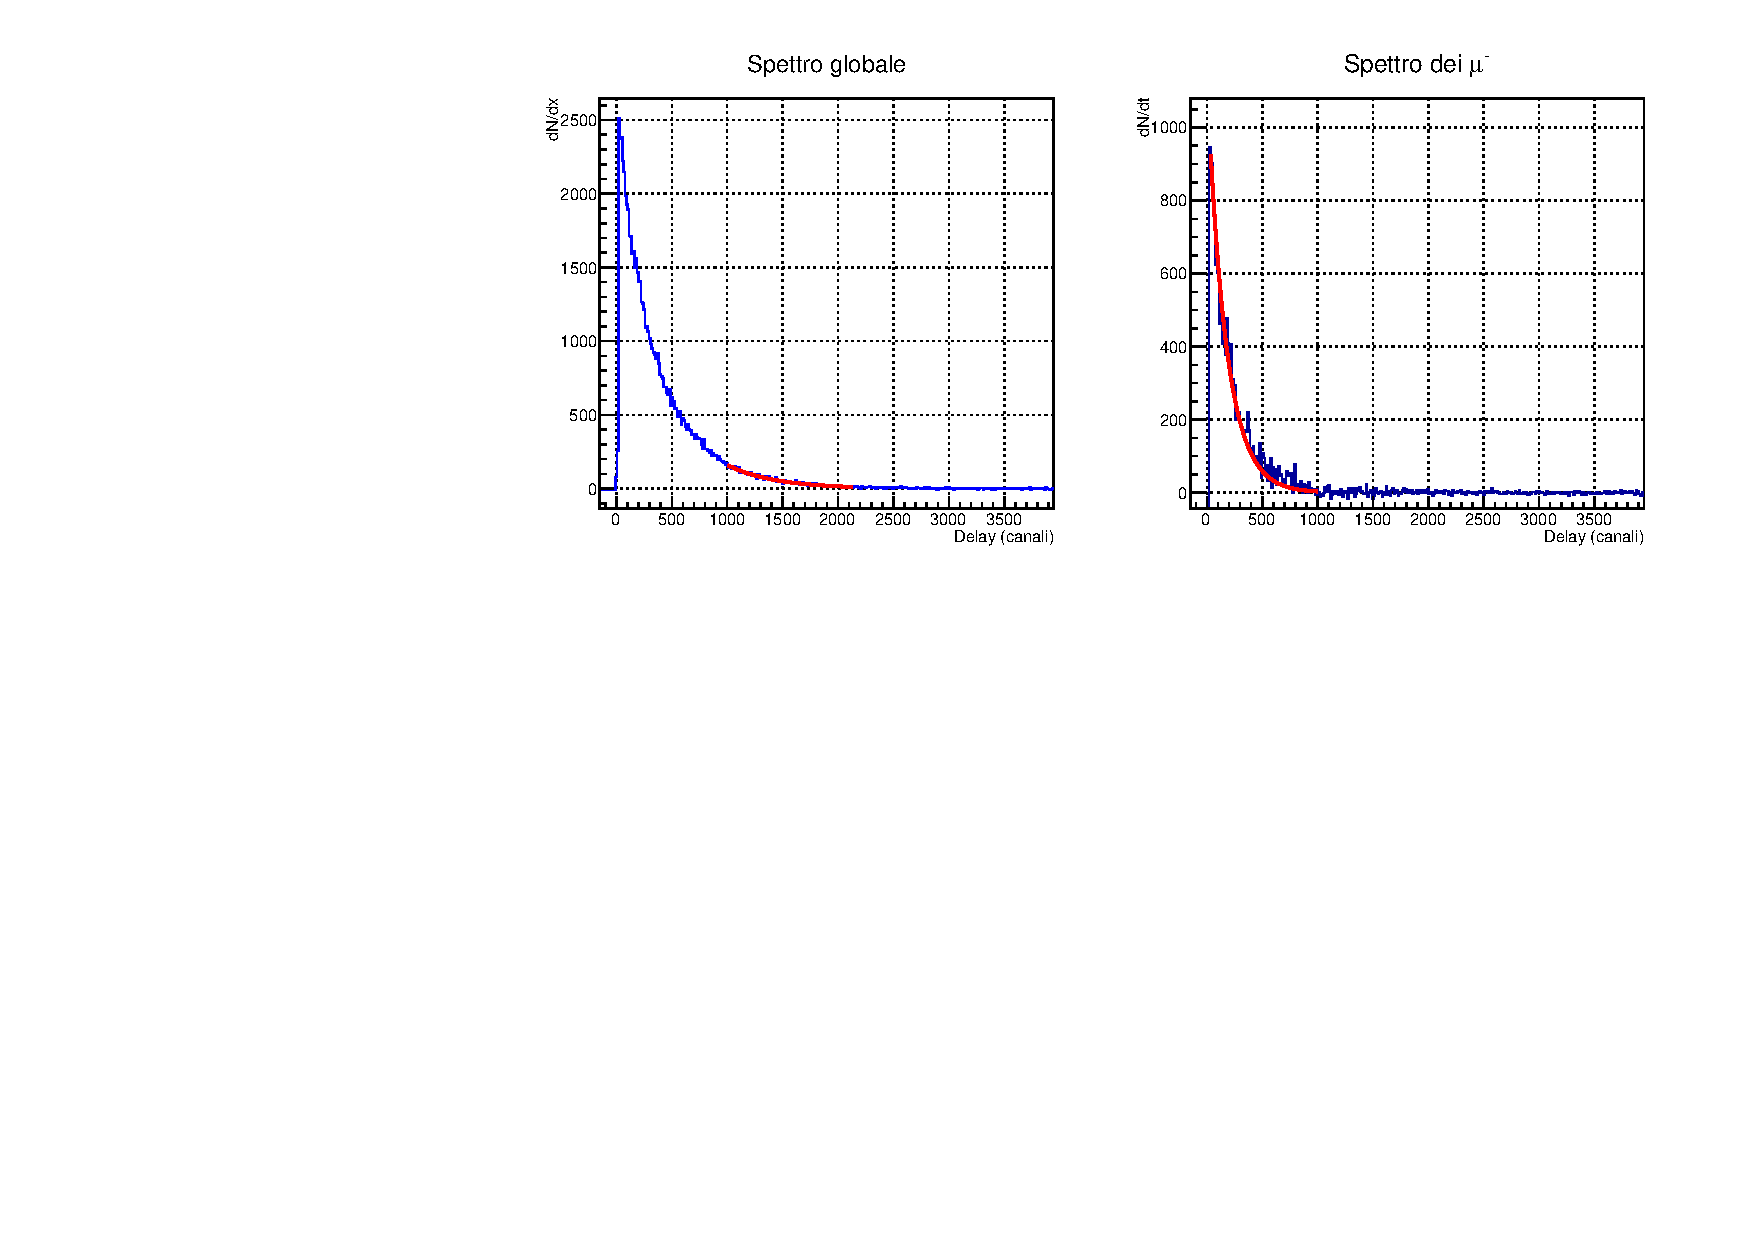
\includegraphics[width=1\textwidth]{img/Spettro_rebin12.pdf}} \\
\subfloat[][{Istogrammi sovrapposti}.]
{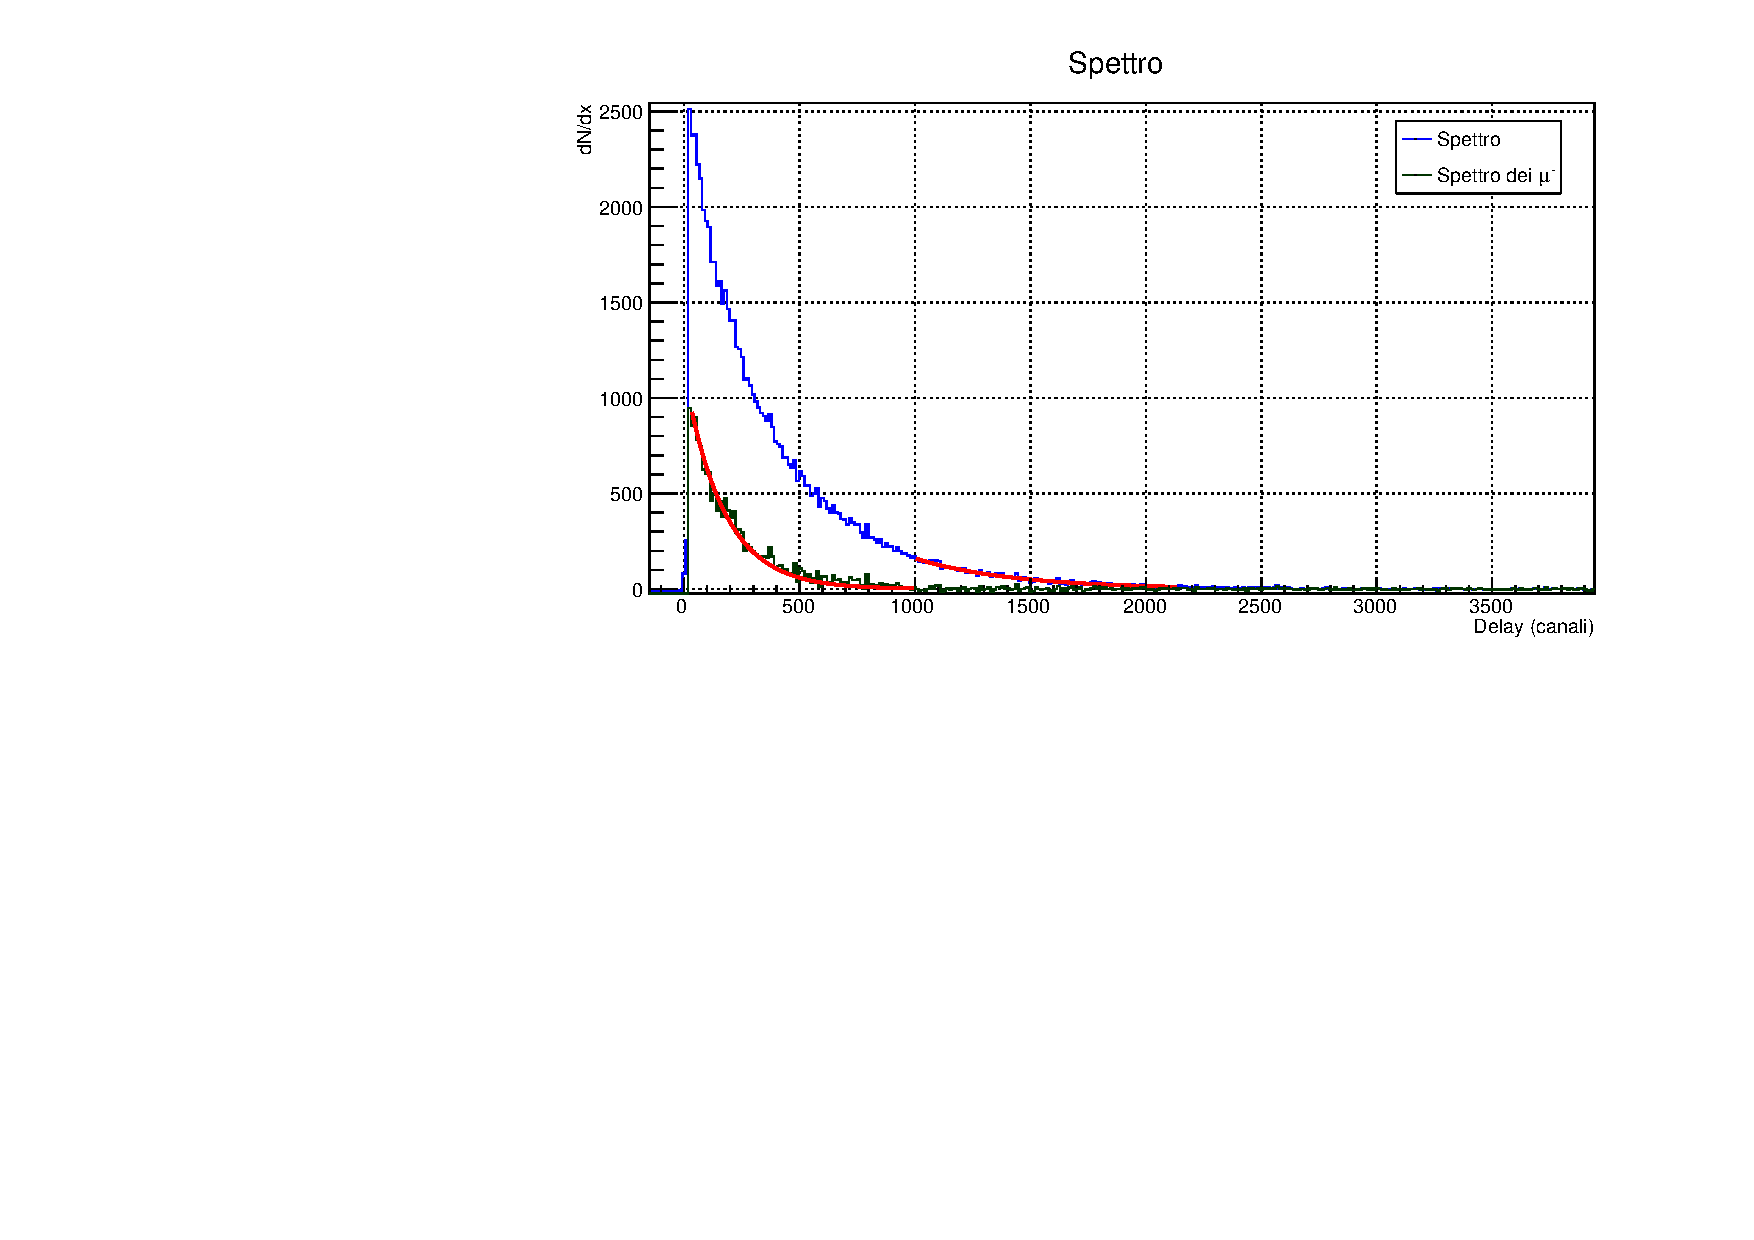
\includegraphics[width=1\textwidth]{img/histo_sovrapposti.pdf}} \\
\caption{Istogrammi dei dati raccolti e analizzati secondo quanto spiegato precedentemente, con un coefficiente di \emph{rebin} 12.}
\label{fig::histo}
\end{figure}
%

In figura~\ref{fig::histo} viene riportato il grafico degli eventi raccolti, dove l'istogramma ha un numero di \emph{bin} diviso per un fattore 12 rispetto a quello originale per ridurre le fluttuazioni statistiche in maniera ottimale; i risultati derivanti da questa analisi sono riportati in tabella~\ref{results}.
%
\begin{table}[H]
	\centering
	\begin{tabular}{cccc}
		\toprule
				& Misura	& Valore atteso 	& Compatibilità \\	
		\midrule
		$\tau^+$	& $(2.20 \pm 0.05) \ \mu \mbox{s}$ 	& $(2.1969811 \pm 0.0000022) \  \mu \mbox{s}$ 	& 0.06 	\\
		$\tau^-$	& $(0.870 \pm 0.007)  \ \mu \mbox{s}$ 	& $(0.8646 \pm 0.0012)  \ \mu \mbox{s}$ 		& 0.76	\\
		$N^+/N^-$	& $1.5 \pm 0.1$ 	& $1.261 \pm 0.009$ 		& 2.38	\\
		\bottomrule
	\end{tabular}
	\caption{Risultati dell'analisi preliminare. Valore atteso di $R$ da \cite{R}.}
	\label{results}
\end{table}
%
%\begin{table}[h!]
%	\centering
%	\begin{tabular}{ccccc}
%		\toprule
%		& Misura [$\mu$s]	&	Valore atteso [$\mu$s]	 & Compatibilità & Differenza [$\mu$s]	\\	
%		\midrule
%		$\tau^+$	&	$2.20\pm 0.05$ & $2.1969811 \pm 0.0000022$ & 0.16 & 0.0072134	\\
%		$\tau^-$	&	$0.870\pm 0.007$ & $0.88 \pm 0.01$ & 0.80 & 0.01	\\
%		$N^+/N^-$	&	$1.5 \pm 0.1$ & $1.261 \pm 0.009$ & 1.95 & 0.20	\\
%		\bottomrule
%	\end{tabular}
%	\caption{Risultati dei fit (rebin 12).}
%	\label{results}
%\end{table}
%%%%%%%%%%%%%%%%%%%%%%%%%%%%%%%%%%%%%%%%%%%%%%%%%%%%%%%%%%%%%%%%%%%%%%%%%%%%%%%%%%%%%%%%%%%%%%%%%%%%%%%%%%%%%%%%%%%%%%%%%%%%%%%%%%%%%%%%%%%%%%%%%%%%%%%%%%%%%%%%%%%%%%%
\cleardoublepage
\section{Simulazioni Monte Carlo}
Lo scopo di questa fase dell'esperimento consiste nella ricerca e messa a punto di un metodo sperimentale di analisi degli spettri raccolti. Il lavoro si suddivide in due passaggi:
\begin{enumerate}
 \item sviluppare un codice di simulazione Monte Carlo in ambiente ROOT \cite{root} nel quale si simulano molti spettri di decadimento dei muoni cosmici in un intervallo utile di circa 3900 canali, in accordo con quelli acquisiti. Gli istogrammi simulati vengono quindi utilizzati per studiare diversi metodi di fit per l'estrazione dei parametri fisici;
 \item utilizzare il metodo di fit stabilito nel passaggio precedente per estrarre $\tau^+$, $\tau^-$ e $R=N^+/N^-$ dagli spettri raccolti.
\end{enumerate}
%
\subsection{Simulazione del fondo}
La prima versione del metodo Monte Carlo prevede la simulazione di spettri costituiti da solo rumore di fondo (detto \textit{baseline}, avente una distribuzione uniforme su tutto l'intervallo), attraverso la generazione uniforme di numeri casuali tramite la funzione \lstinline{TRandom3::Uniform}. I metodi studiati per la stima della \textit{baseline} sono i seguenti:
\begin{enumerate}
 \item media aritmetica dei contenuti dei \emph{bin} dell'istogramma;
 \item fit con il metodo del $\chi^2$ utilizzando la funzione \lstinline{pol0} (\lstinline{TH1::Fit("pol0")});
 \item metodo della \textit{maximum likelihood} utilizzando la funzione \lstinline{pol0} \newline (\lstinline{TH1::Fit("pol0","L")}).
\end{enumerate}

In figura \ref{fig::baseline_500} è riportato un esempio delle distribuzioni dei valori e degli errori derivanti da simulazioni multiple, stimati con i tre metodi. La linea verde verticale nei grafici indica il valore vero della \textit{baseline}, ossia quello con cui sono stati simulati gli spettri, e perciò la stima che dovrebbe essere restituita dall'analisi. Come si può notare, la distribuzione dei valori estratta con fit \lstinline{pol0} con il metodo del $\chi^2$ non è centrata attorno al valore atteso: in questo caso, infatti, la \textit{baseline} è sistematicamente sottostimata, poichè il metodo dei minimi quadrati non funziona correttamente per il fit di un istogramma con \emph{bin} a bassa statistica aventi come errore la radice del contenuto. Inoltre, il fit di una \lstinline{pol0} con il metodo del $\chi^2$ corrisponde esattamente ad una media pesata, nella quale i \emph{bin} con statistica minore hanno un peso maggiore, con conseguenti valori sottostimati della \textit{baseline}\footnote{Media pesata e relativo errore:
$$\bar{b}=\frac{\sum_{i=1}^N b_i/\sigma_i^2}{\sum_{i=1}^N 1/\sigma_i^2};
\hspace{1cm} \sigma_{\bar{b}}=\frac{1}{\sum_{i=1}^N1/\sigma_i^2}$$}. In virtù di queste considerazioni, il metodo di fit del $\chi^2$ è stato scartato. 

Le distribuzioni relative agli errori statistici sulla \textit{baseline} sono utili per controllare che le stime dei valori non abbiano dispersione troppo elevata attorno al valor medio; in altre parole, si effettua il confronto tra la $\sigma$ delle gaussiane dei valori e il centroide $\overline{\sigma_{b}}$ delle gaussiane degli errori, controllando che siano dello stesso ordine di grandezza. In particolare, nelle simulazioni in esame risulta che $\sigma\lesssim \overline{\sigma_{b}}$: questa condizione garantisce che, scegliendo $\overline{\sigma_{b}}$ come incertezza sulla \textit{baseline}, non si stia introducendo alcuna componente sistematica di errore. Dato che inoltre risulta che il metodo della media ha una dispersione attorno al centroide leggermente più alta rispetto al metodo della \textit{likelihood}, si preferisce da qui in poi l'utilizzo di quest'ultimo.
%
\begin{figure}[H]
 \centerline{\includestandalone[width=\linewidth+1cm]{img/baseline}}
 \caption{Distribuzioni delle stime della \textit{baseline} con i tre metodi differenti, sia per i valori sia per i relativi errori (500 simulazioni). La \textit{baseline} generata in queste simulazioni ha altezza 10 conteggi.}\label{fig::baseline_500}
\end{figure}
%
\subsection{Simulazione del fondo e del primo esponenziale} \label{bexp}
La fase successiva dello sviluppo del metodo Monte Carlo prevede di studiare una distribuzione contenente un termine costante sommato a un termine esponenziale: 
\begin{equation}
 f(t;A,\tau,b)=Ae^{-\frac{t}{\tau}}+b \ .
 \label{eq::exp_plus_base}
\end{equation}
Per la costruzione degli spettri si è scelto di generare indipendentemente la distribuzione uniforme con \lstinline{TRandom3::Uniform} e la distribuzione esponenziale con \lstinline{TRandom3::Exp}, per poi sommarle. Avendo stabilito che il metodo della \textit{maximum likelihood} è il più accurato si sono studiati diversi approcci al fit degli spettri:
\begin{enumerate}
  \item fit diretto con la funzione completa impostando $\tau$ al valore vero e lasciando $A$ e $b$ non inizializzati;
  \item fit di tipo \lstinline{pol0} della parte finale dello spettro per la stima di $b$, utilizzata in secondo luogo per inizializzare il corrispondente parametro del fit nella funzione completa del metodo precedente;
  \item fit di tipo \lstinline{pol0} della parte finale dello spettro per la stima di $b$, quindi sottrazione della componente costante della distribuzione e successivo fit puramente esponenziale.
\end{enumerate}
Dei tre metodi, il secondo si è rivelato il più stabile: un fit a tre parametri come nel primo metodo, infatti, necessita di inizializzare i valori di partenza in modo che siano sufficientemente vicini a quello vero affinchè l'algoritmo di massimizzazione della \textit{likelihood} vada a convergenza correttamente; ciò porta a preferirgli il secondo metodo, più stabile con valori iniziali distanti dal valore vero. Anche il terzo metodo presenta delle criticità rispetto al secondo: in primo luogo, una sottrazione di dati può facilmente portare ad avere canali a contenuto negativo (privi di significato fisico); in secondo luogo, come si può notare dalla figura~\ref{baselinestart}, il fit della \textit{baseline} sovrastima il valore di $b$ e perciò la sottrazione potrebbe comportare un errore sistematico nel fit successivo.

L'adozione del secondo metodo richiede la scelta del canale (valore di ritardo temporale) dal quale far iniziare il fit della porzione di \textit{baseline}: si è quindi proceduto a eseguire uno studio sistematico dei risultati al variare di questo estremo inferiore, confrontando le medie su più simulazioni (figura~\ref{baselinestart}). Dal grafico è evidente come la riscostruzione sia più precisa, ma meno accurata, per piccoli valori dell'estremo, e di come la situazione si inverta per grandi valori di esso. A priori si potrebbe scegliere un valore che rappresenti la via di mezzo tra queste due situazioni, ma a posteriori, studiando la ricostruzione di $b$ e $\tau^+$ dopo il fit esponenziale del metodo 2, si è verificato con varie prove come la scelta di questo valore iniziale sia del tutto ininfluente sulla bontà della convergenza ai parametri impostati in \textit{input}; per questo motivo, si è scelto come estremo il valore in canali corrispondente a $6\tau^+\sim13\ \mu$s, dopo il quale la popolazione di $\mu^+$ è pressochè assente.

%
\begin{figure}[h]
  \centerline{\includestandalone[width=\linewidth+1cm]{img/tprofile}}
  \caption{Studio della ricostruzione della \textit{baseline} $b$ al variare del punto di inizio del fit di tipo \texttt{pol0}: in alto i valori ottenuti (la linea rossa rappresenta il valore vero) e in basso i rispettivi errori. Le barre di errore rappresentano la deviazione standard del campione di 100 simulazioni. I dati utilizzati nella generazione corrispondono a 1 settimana di acquisizione.}\label{baselinestart}
\end{figure}
%
\subsection{Simulazione del fondo e di entrambi gli esponenziali}\label{bexpexp}
Il metodo Monte Carlo prevede ora di studiare una distribuzione contenente un termine costante di \textit{baseline} e due esponenziali:
\begin{equation}
 f(t;A_+,\tau^+,A_-,\tau^-, b)=A_-e^{-\frac{t}{\tau^-}}+A_+e^{-\frac{t}{\tau^+}}+b\ .
 \label{eq::funzione_fit_finale}
\end{equation}
La distribuzione esponenziale relativa ai $\mu^-$ viene generata con \lstinline{TRandom3::Exp} separatamente da quella dell'esponenziale dei $\mu^+$ e della \textit{baseline}, sommando infine le distribuzioni in un unico istogramma, come nel \S\ref{bexp}. 

L'adozione del metodo 2 descritto in precedenza prevede uno studio accurato del canale (quindi del ritardo temporale) dal quale cominciare il fit della funzione $A_+e^{-\frac{t}{\tau^+}}+b$. 
\begin{figure}[b!]
  \centerline{\includestandalone[width=\linewidth+1cm]{img/fitbegin_5week_100sim}}
  \caption{Studio della stima di $\tau_+$ al variare del punto di inizio del fit $A_+e^{-\frac{t}{\tau^+}}+b$. La linea rossa rappresenta il valore vero impostato nella simulazione. Le barre d'errore rappresentano la deviazione standard del campione di 100 simulazioni utilizzate. I dati utilizzati nella generazione corrispondono a 5 settimane di acquisizione.}
  \label{fig::tauplusstart}
\end{figure}
Come riportato in figura~\ref{fig::tauplusstart}, questo fit produce un valore di $\tau^+$ che è sempre sottostimato rispetto al valore vero: tuttavia, dato che si è verificato come la scelta di questo estremo non influenzi il fit successivo (comprendente anche il secondo esponenziale), si è scelto un valore in canali corrispondente a $5\tau^-\sim4.4\ \mu$s, dopo il quale la popolazione di $\mu^-$ è pressochè assente.

Il metodo di fit messo a punto prevede i seguenti passaggi:
\begin{enumerate}
 \item fit di tipo \lstinline{pol0} della coda dello spettro con estrazione del valore preliminare (denotato con $B$) per la \textit{baseline};
 \item definizione della funzione corrispondente alla formula~\ref{eq::exp_plus_base}, inizializzazione del parametro $b$ al valore $B$ derivante dal fit del punto precedente (\lstinline{TF1::SetParameter("b",B)}) e realizzazione del fit dell'istogramma a partire da un ritardo di $5\tau^-$ (in questo modo si ottengono le stime intermedie $\widetilde{\tau}$  e $\widetilde{B}$ per i parametri $\tau^+$ e $b$, rispettivamente);
 \item definizione della funzione complessiva di fit corrispondente alla formula~\ref{eq::funzione_fit_finale}, inizializzazione dei parametri $\tau^+$ e $b$ ai valori  $\widetilde{\tau}$ e $\widetilde{B}$ e, infine, fit dell'istogramma, con estrazione dei valori definitivi dei parametri. 
%
\end{enumerate}  
Concludendo, la generazione degli spettri utilizza i parametri di \textit{input} $\{\tau^+,\tau^-,R,b,I\}$, dove $I$ è l'integrale della distribuzione. Questi parametri sono tra loro legati dalle seguenti relazioni:
\begin{equation*}
  \begin{cases}
    I = \int\limits_{t_0}^\infty f(t)dt = A_-\tau^-e^{-t_0 / \tau^-} + A_+\tau^+e^{-t_0 / \tau^+} + b\cdot r \\
    R = \frac{A^+}{A^-} \\
  \end{cases}
  \label{eq::condizioni_parametri}
\end{equation*}
dove 
\begin{itemize}
 \item $f(t) = \d N/\d t$ corrisponde alla formula~\ref{eq::funzione_fit_finale};
 \item $t_0$ corrisponde all'istante in cui inizia l'istogramma (per una discussione più completa riguardo a questo valore si rimanda al \S\ref{analPrelim});
 \item $r$ è l'intervallo di definizione dell'istogramma (circa 4000 canali);
 \item $I$ e $b$ sono vincolati, in quanto uno sguardo allo spettro reale suggerisce che una settimana di acquisizione corrisponde a circa 80000 eventi e a $b\sim1 $.
\end{itemize}
Di seguito viene riportato un esempio di spettro generato e analizzato come descritto.

\begin{figure}[h]
 \centerline{\includestandalone[width=\linewidth+1cm]{img/example_single_spectrum}}
 \caption{Esempio di istogramma simulato con statistica associata a 5 settimane di acquisizione ($b\sim5$) con sovrapposta la funzione di fit corrispondente. I parametri di \textit{input} $\tau^+$, $\tau^-$ e $R$ sono quelli della letteratura.}
 \label{fig::esempio_spettro_simulato}
\end{figure}
%
\subsection{Test multipli del metodo di fit}
Sino ad ora, si è testato e messo a punto il metodo di fit sulla base di spettri simulati con i valori attesi dei parametri, in particolare $\tau^+  \simeq 2.19  \ \mu s$ $(\sim 429$ canali$)$, $\tau^- \simeq 0.86 \  \mu s$ $(\sim 172$ canali$)$ e $R\simeq1.26$. 
In questa fase si intende testare il metodo su distribuzioni simulate con diversi valori in \textit{input}, anche senza alcun senso fisico: lo scopo è quello di avvalorarne la correttezza, verificando cioè che esso sia in grado di restituire in \textit{output} stime dei parametri compatibili con i valori in \textit{input}.

\newpage La strategia adottata si sviluppa in due fasi:
\begin{enumerate}
 \item fissato un insieme di parametri di \textit{input}, si generano 500 spettri di cui viene in seguito effettuato il fit con il metodo precedentemente descritto. Le stime dei parametri fornite dal fit e i relativi errori vengono immagazzinati all'interno di nuovi istogrammi; ci si aspetta che questi siano centrati attorno al valore del parametro inserito in \textit{input} alla simulazione. Tali istogrammi vengono riempiti esclusivamente dai fit che restituiscono stime dei parametri soddisfacenti le seguenti condizioni di qualità:
 \begin{itemize}
  \item errore relativo inferiore al $20\%$;
  \item compatibilità con il valore atteso entro le $3\sigma$. 
 \end{itemize}
 Se le stime del fit di uno spettro non soddisfano almeno una di queste condizioni per almeno uno dei parametri $\tau^+$, $\tau^-$ e $R$, nessuno degli istogrammi viene riempito per quella particolare simulazione; si riporta un esempio in figura \ref{fig::esempio_set_simulazioni}.
%
\begin{figure}[b!]
  \centering
  \includestandalone[width=\linewidth]{img/single}
  \caption{Esempio di distribuzioni dei valori estratti dal fit dei singoli parametri e dei relativi errori, derivanti da 500 simulazioni con parametri impostati ai valori fisici; le linee verdi indicano il valore di ogni parametro di \textit{input}. La statistica relativa ad ogni singolo spettro è comparabile con quella di 1 settimana di acquisizione ($ 80000$ eventi, $b\sim1$). L'efficienza finale del metodo per questa specifica simulazione è del $96.8\%$, il che vuol dire che in 16 (su 500) simulazioni almeno uno dei parametri ($\tau^+$, $\tau^-$, $R$) non ha rispettato almeno una condizione di quelle elencate; per questo passaggio, non si è indagato quale parametro o quale condizione fallisse, ritenendosi soddisfatti dall'alta efficienza raggiunta.}
  \label{fig::esempio_set_simulazioni}
 \end{figure}
 
 \item Si ripete la procedura del punto precedente con campioni di 500 simulazioni ottenuti con parametri di \textit{input} di volta in volta diversi. Ogni campione contribuisce all'efficienza complessiva sulla base delle stime di $\tau^+$, $\tau^-$ e $R$ corrispondenti ai centroidi delle distribuzioni dei valori, ai quali, come incertezza, si assegna il centroide $\sigma$ della rispettiva distribuzione degli errori. In particolare, le condizioni di qualità che devono essere soddisfatte sono:  
 \begin{itemize}
  \item errore relativo inferiore al $20\%$;
  \item compatibilità con il valore atteso entro le $3\sigma$;
  \item modulo della differenza tra la dispersione ($\bar{\sigma}$) della distribuzione dei parametri e centroide della distribuzione degli errori inferiore del minore dei due. Questo tipo di condizione permette di controllare la presenza di eventuali errori sistematici qualora $\bar{\sigma}$ fosse ordini di grandezza maggiore rispetto al centroide $\sigma$ della distribuzione degli errori.  
 \end{itemize}
Qualora almeno una di queste condizioni non sia soddisfatta per almeno uno dei parametri $\tau^+$, $\tau^-$ e $R$ il campione viene rigettato; in caso contrario, si considera valido. 
\end{enumerate}
Si è deciso di applicare la procedura descritta facendo variare i valori di \textit{input} dei parametri $\tau^+$, $\tau^-$ e $R$ del $40\%$ attorno al valore fisico, considerando statistiche corrispondenti a 1, 3, 5 settimane di acquisizione, per un totale di $3^4=81$ campioni rispetto ai quali calcolare l'efficienza; in virtù di questi test, si è prodotto il grafico in figura \ref{fig:eff1}.
%
\begin{figure}[b!]
  \centering
  \includestandalone[width=\linewidth]{img/matrix_eff40}
  \caption{Efficienza del metodo per una variazione dei parametri del $40\%$ rispetto al valore fisico; si noti che ciò che più spesso fallisce è la stima di $R$.}
  \label{fig:eff1}
\end{figure}
%
Prestando ulteriore attenzione, si sono osservate alcune criticità:
\begin{itemize}
 \item nel caso di campioni generati con valori di $\tau^+$ e $\tau^-$ ravvicinati, distanti circa $0.8 \ \mu s - 0.9 \ \mu s$, il metodo di fit fallisce, non riuscendo ad andare a convergenza. Questo problema riguarda comunque campioni di dati relativi a spettri molto diversi da quelli raccolti (le vite medie ``lunghe'' e ``corte'' non sono più tali);
 \item il parametro $R$ è quello più difficile da stimare correttamente, risultando determinante per rigettare alcuni campioni per i quali le stime di $\tau^+$ e $\tau^-$ sono comunque valide.  
\end{itemize}
Per evidenziare queste criticità, sono stati variati i parametri in intervalli sempre più estesi (dal $10\%$ al $50\%$), producendo il grafico in figura \ref{fig:finalematrix}: appare evidente come l'efficienza peggiori aumentando il range di variazione, avallando l'ipotesi secondo la quale una efficienza non ottimale sia da ricondursi a parametri troppo distanti dai valori veri (e, per i $\tau$, troppo vicini tra loro) più che a difetti del codice. Rimane comunque evidente come $R$ sia il parametro più problematico: ogni tentativo di miglioramento del metodo, come per esempio l'affinamento della scelta dei parametri da impostare con \lstinline{TF1::SetParameter} e l'impostazione di parametri aggiuntivi quali $A_+$ e $A_-$ nei fit preliminari, non è tuttavia riuscito a innalzare l'efficienza.
%
\begin{figure}[H]
  \centering
  %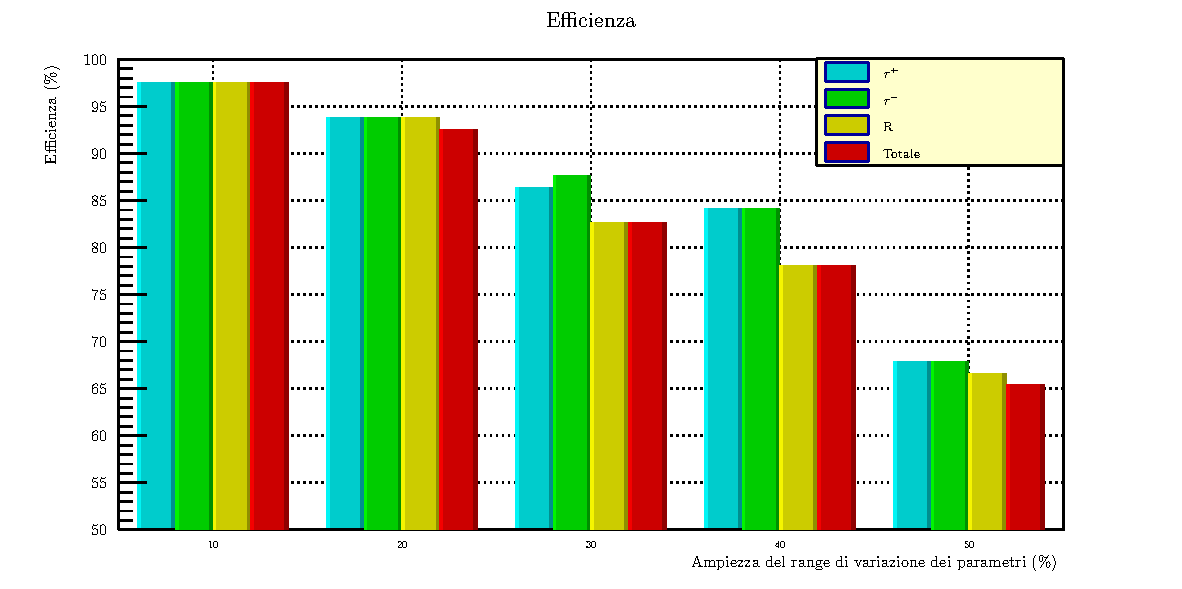
\includegraphics[width=\linewidth+1cm]{img/matrix_5run.pdf}
  \includestandalone[width=\linewidth+1cm]{img/matrix_5run}
  \caption{Efficienza del metodo per una variazione dei parametri dal $10 \%$ al $50\%$ rispetto al valore fisico; si noti l'andamento decrescente all'aumentare del range di variazione.}
  \label{fig:finalematrix}
\end{figure}
%
%
\subsection{Studio del fattore di \emph{rebin}} \label{parrebin}
Durante l'analisi è stata presa in considerazione l'idea di applicare un'operazione di \textit{rebinning} (ovvero la fusione di un certo numero di canali adiacenti, specificato dal \textit{fattore di rebin}, atta alla creazione di un unico \emph{bin} che ha come altezza la somma delle precedenti) all'istogramma dei dati, originariamente costituito da 4096 canali, prima dell'applicazione del metodo di fit. Il \textit{rebinning} era stato adottato in precedenza nel \S\ref{analPrelim} nell'ambito dell'analisi dati preliminare, e sembrava dare stabilità e maggiore accuratezza ai risultati del fit: la conseguenza principale del \textit{rebinning} è infatti quella di smorzare le fluttuazioni statistiche, e perciò l'efficacia dell'operazione ai fini del processo di analisi dei dati deve essere sistematicamente investigata.

Innanzitutto, si è applicata l'operazione a simulazioni Monte Carlo convergenti e accurate con valori del fattore di \emph{rebin} pari a 2, 4, 8, 16, non riscontrando miglioramenti evidenti nella ricostruzione dei paramentri di fit, nonché nella larghezza delle loro distribuzioni. Si è quindi proceduto a verificare l'eventualità in cui un'operazione di \textit{rebinning} potesse rendere convergente un fit non convergente, attestando anche in questo frangente una sostanziale ininfluenza del metodo.

In conclusione, si può tranquillamente assumere l'operazione di \textit{rebinning} come assolutamente ininfluente ai fini dell'analisi dati.
%
\section{Analisi dello spettro reale} \label{analisireale}
Il campione di dati corrisponde agli eventi raccolti in 33 giorni di acquisizione, per un totale di 375241 eventi (frequenza $\sim0.13$ Hz). I risultati sono presentati in tabella \ref{risultatiFinali} e in figura~\ref{fig:finale}.

L'ultimo punto lasciato in sospeso è la questione, menzionata nel \S\ref{tac}, dell'eccesso di eventi registrato con le coincidenze artificiali nell'intervallo $[2200,2700]$ canali; nell'istogramma finale non si nota alcuna sovrabbondanza di eventi nel suddetto intervallo, corrispondente ai ritardi nel \emph{range} $[11 \ \mu \mbox{s}, 14 \ \mu \mbox{s}]$. In ogni caso, sono stati tentati due approcci per tenerne conto nell'analisi dati:
\begin{enumerate}
  \item \textbf{esclusione dal fit,} ovvero si è costruita una funzione di fit alternativa definita a tratti tramite \lstinline{TF1::RejectPoint}, che esclude i punti dal calcolo della \textit{likelihood};
  \item \textbf{errori incrementati,} ovvero si è provato a attribuire errori maggiori ai punti nell'intervallo, ad esempio il doppio rispetto all'errore poissoniano standard.
\end{enumerate}
Nessuno dei due metodi ha portato a differenze osservabili nei risultati finali.
%
\section{Discussione dei risultati}

La tabella~\ref{risultatiFinali} mostra come, a fronte di un'ottima compatibilità per i valori dei $\tau$ rispetto a quelli attesi, $R$ risulti notevolmente sovrastimato: avendo già escluso che ciò possa essere in qualche modo influenzato dallo spettro raccolto (o dal metodo di fit), è stato effettuato un tentativo di analisi dell'energia delle particelle incidenti.

Infatti, $R$ dipende dall'energia dei muoni incidenti \cite{pb}, ed è possibile inferire che per arrivare ad avere un valore attorno a 1.6, compatibile con quello ottenuto in tabella~\ref{risultatiFinali}, $E_{\mu} \sim 10$ TeV: tuttavia, per frenare un muone di tale energia con del piombo \cite{pdg}, prendendo come densità $ \rho_{Pb} = 11.3 $ g/cm$^3$, servirebbero quasi 5 km di spessore, a fronte dei 20 cm presenti in laboratorio. Per questo motivo, si scarta anche questa ipotesi. %lasciando aperta l'unica possibilità che tale discrepanza dipenda dall'apparato di raccolta dati, come gli scintillatori
%
\newpage
\begin{table}[h]
	\centering
	\begin{tabular}{cccc}
		\toprule
				& Misura	& Valore atteso 	& Compatibilità \\	
		\midrule
		$\tau^+$	& $(2.18 \pm 0.02) \ \mu \mbox{s}$ 	& $(2.1969811 \pm 0.0000022) \  \mu \mbox{s}$ 	& 0.64 	\\
		$\tau^-$	& $(0.85 \pm 0.04)  \ \mu \mbox{s}$ 	& $(0.8646 \pm 0.0012)  \ \mu \mbox{s}$ 		& 0.36	\\
		$N^+/N^-$	& $1.80 \pm 0.09$ 	& $1.261 \pm 0.009$ 		& 6.10	\\
		\bottomrule
	\end{tabular}
	\caption{Risultati del metodo di fit studiato applicato allo spettro reale.}
	\label{risultatiFinali}
\end{table}
%
\begin{figure}[h]
 \centerline{%
  \includestandalone[width=\linewidth+1.2cm]{img/finaleres}}
  \caption{In alto, il risultato del fit sullo spettro dei dati acquisiti; in basso, il grafico dei residui. I colori indicano i diversi intervalli di ritardo temporale corrispondenti ai passaggi del metodo di analisi adottato (come descritto nel \S\ref{bexpexp}).}
  \label{fig:finale}
\end{figure}
%
\appendix
%\setcounter{secnumdepth}{0}
\section{Previsioni teoriche}
Nei paragrafi successivi sono riportati due diversi approcci, uno analitico e uno computazionale, per tentare di stimare la percentuale di eventi passati in coincidenza attraverso due \emph{slab} di area uguale, pari a $S=L \cdot D = 1.83 \ \mbox{m} \cdot 0.2 \ \mbox{m} =0.366$ m$^2$, e distanti verticalmente di una quantità pari a $h$; tale parametro permette di scegliere la coppia di \emph{slab} di cui si vogliono valutare gli eventi in coincidenza, e nei conti che seguono si è assunto $h=0.08$ m, ovvero la distanza tra S1 e S2.

Il conto è stato effettuato considerando le \emph{slab} monodimensionali, bidimensionali e, per la simulazione, anche tridimensionali, cioè considerandone lo spessore; i risultati ottenuti sono in buon accordo fra di loro e con i dati sperimentali.
\subsection{Calcolo analitico del numero di coincidenze attese tra due \emph{slab} parallele}
\subsubsection{Caso unidimensionale}
La situazione è quella riportata nell'immagine che segue:
\newline

\begin{tikzpicture}
	\newcommand\dz{0.2}
	\newcommand\dpmt{0.03}
	
	\node at (1,\dz/2) {S2};
	\draw[fill=black!25!white] (2,0-\dpmt) rectangle (10,\dz+\dpmt);
	\node at (6,-0.4) {0};
	\node at (8.7,-0.25) {x};

	\node at (1,1+\dz/2) {S1};
	\draw[fill=black!25!white] (2,1-\dpmt) rectangle (10,1+\dz+\dpmt);
	
	\draw (4,2) -- (8.7,\dz+\dpmt);
	\draw (8.7, \dz+\dpmt) -- (8.7,2);
	\draw (5, 1.63) -- (4.95, 1.73);
	\draw (5, 1.63) -- (4.9, 1.58);
	
	
	\draw [dashed] (2, 1-\dpmt) -- (8.7, \dz+\dpmt);
	\draw [dashed] (8.7, \dz+\dpmt) -- (10,1);
	
	\node at (8.4,0.65) {$\theta$};
	
	\draw (8.7, 0.5) arc [radius=0.4, start angle=90, end angle= 141];
	
	\draw (6,-\dpmt) -- (6,-0.2);
	\draw (8.7,-\dpmt) -- (8.7,-0.1);
	
	\draw [->] (1.5,-0.7) -- (11,-0.7);
\end{tikzpicture}
\newline

Il numero di eventi passati per la \emph{slab} superiore è $$N = \alpha \cdot T \cdot \int_{-\frac{L}{2}}^{\frac{L}{2}} dx \cdot \int_{-\frac{\pi}{2}}^{\frac{\pi}{2}} \cos ^2\theta d\theta $$e questo permette di fissare il valore della costante $$\alpha = \frac{2N}{\pi LT}$$
dove $T$ è il tempo di acquisizione. Ora, si osserva che su un punto sulla \emph{slab} inferiore corrispondente a $0<x<\frac{L}{2}$ arrivano gli eventi compresi fra due angoli $$\theta = -\arctan \bigg(\frac{\frac{L}{2}-x}{h}\bigg) \equiv \theta_1$$ e $$\theta = \arctan \bigg(\frac{\frac{L}{2}+x}{h}\bigg) \equiv \theta_2\;.$$ 
Data la simmetria del problema, si ottiene facilmente che la situazione è analoga per valori di $x$ negativi; si può allora scrivere che il numero di eventi passati per la \emph{slab} inferiore è $$N' =\alpha \cdot T \cdot \int_{-\frac{L}{2}}^{\frac{L}{2}} dx \int_{-\theta_1}^{\theta_2}  \cos ^2\theta d\theta$$ da cui si ricava subito $$\frac{N'}{N}=\frac{2}{\pi L} \int_{-\frac{L}{2}}^{\frac{L}{2}} dx \int_{-\theta_1}^{\theta_2}  \cos ^2 \theta d\theta \simeq 97.22 \%. $$ Tale valore è in ottimo accordo con la simulazione eseguita successivamente.

\subsubsection{Caso bidimensionale}
La situazione è ora quella riportata nelle due figure che seguono:
\newline

\begin{figure}[h]
\subfloat[Visione laterale.]{

\begin{tikzpicture}
	\newcommand\dz{0.2}
	\newcommand\dpmt{0.03}
	
	\node at (1.5,\dz/2) {S2};
	\draw[fill=black!25!white] (2,0-\dpmt) rectangle (8,\dz+\dpmt);
	
	\node at (1.5,1+\dz/2) {S1};
	\draw[fill=black!25!white] (2,1-\dpmt) rectangle (8,1+\dz+\dpmt);
	
	\draw (2,\dz+\dpmt) -- (2,1+\dz+\dpmt+0.7);
	\draw (2, \dz+\dpmt) -- (8.3,1+\dz+\dpmt+0.4);
	
	\draw (6.45,1+\dz+\dpmt) circle[radius=2pt];
	\fill (6.45,1+\dz+\dpmt) circle[radius=2pt];
	
	\draw (7.5,1+\dz+\dpmt+0.21) -- (7.55,1+\dz+\dpmt+0.29);
	\draw (7.5,\dz+\dpmt+1.21) -- (7.6,1+\dz+\dpmt+0.195);
	
	\node at (2.52,0.75) {$\theta_\text{max}$};
	
	\draw (2.25,0.1+\dz+\dpmt) arc [radius=0.25, start angle=0, end angle= 85];
		
	\draw [->] (1,-0.5) -- (1,1+\dz+\dpmt+1);
	
	\node at (1.35,1+\dz+\dpmt+0.7) {z};
\end{tikzpicture}}
\hspace{0.4cm}
\subfloat[Visione dall'alto.]{
\begin{tikzpicture}
	\newcommand\dz{0.2}
	\newcommand\dpmt{0.03}
	
	\draw[fill=black!25!white] (2,0.5) rectangle (6.6,1+\dz+\dpmt+0.5);
		
	\draw (2,0.8) -- (5,1.3);
	\draw (5,1.3) circle[radius=2pt];
	\fill (5,1.3) circle[radius=2pt];
	
	\draw (2,0.8) -- (7,0.8);
	
	\node at (4,0.95) {$\phi$};
	
	\draw (3.8,0.8) arc [radius=0.8, start angle=0, end angle= 21];
	
	\draw [->] (1,0) -- (7.75,0);
	\draw [->] (1,0) -- (1,2.7);
	
	\node at (7.25,0.3) {x};
	\node at (1.3,2.45) {y};	
	
\end{tikzpicture}}
\end{figure}

L'origine del sistema di riferimento è stata presa nel punto centrale della \emph{slab}; il pallino nero indica il punto di incidenza del raggio cosmico.

Come per il caso 1D, si fissa intanto la costante di proporzionalità, facendo attenzione al fatto che questa volta bisogna integrare sull'angolo solido, e $\theta\in(0,\frac{\pi}{2})$: 
$$N = \alpha \cdot T \cdot L \cdot D \cdot 2\pi \cdot \int_{0}^{\frac{\pi}{2}} \cos^2\theta  \sin\theta d\theta$$
che fornisce 
$$\alpha = \frac{3N}{2\pi TLD}.$$ 
A questo punto, per valutare il numero di eventi in coincidenza, si inizia l'analisi con $\phi\in(0, \frac{\pi}{2})$, che corrisponde all'evento mostrato nel disegno sopra. Un evento del genere passerà in coincidenza solo se la sua inclinazione è $$\theta \leq \arctan \bigg(\frac{\frac{L}{2}+x}{h\cdot \cos\phi}\bigg) \equiv \theta_1\;,$$ formula valida fino a quando il valore di $\phi$ non è tale da intersecare lo spigolo in basso a sinistra, ovvero $$\phi = \phi^{*} = \arctan \bigg(\frac{\frac{D}{2}+y}{\frac{L}{2}+x}\bigg)\;,$$ oltre il quale l'inclinazione massima è $$\theta = \arctan \bigg(\frac{\frac{D}{2}+y}{h\cdot \sin\phi}\bigg)  \equiv \theta_2\;.$$I raggi cosmici in coincidenza sono quindi dati da questo integrale, moltiplicato per 4, dato che $\phi\in(0, 2\pi)$ e il problema è simmetrico. Tramite una risoluzione numerica si ottiene quindi:
\begin{multline*}
\frac{N'}{N}=4\cdot \alpha \cdot T\cdot \bigg( \int_{-\frac{L}{2}}^{\frac{L}{2}} dx \int_{-\frac{D}{2}}^{\frac{D}{2}} dy \int_0^{\phi^{*}} d\phi \int_0^{\theta_1} \cos^2\theta \sin\theta d\theta +\\
+ \int_{-\frac{L}{2}}^{\frac{L}{2}} dx \int_{-\frac{D}{2}}^{\frac{D}{2}} dy \int_{\phi^{*}}^{\frac{\pi}{2}} d\phi \int_0^{\theta_2} \cos^2\theta \sin\theta d\theta\bigg)\simeq 73.89 \%\;.
\end{multline*} 
Anche questo valore è in buon accordo con i risultati della simulazione 2D.

\subsection{Simulazione del numero di coincidenze}
L'approccio seguito per ogni simulazione è il medesimo: si sono innanzitutto generati $N$ eventi come set di numeri (di cardinalità dipendente dalla dimensione), corrispondenti ai raggi cosmici passanti per la \emph{slab} soprastante, e quindi, con semplici considerazioni geometriche, si sono contati gli eventi passati anche per la \emph{slab} sottostante. Il numero $N$ è stato stimato come il numero di muoni cosmici attesi sulla \emph{slab} soprastante in un tempo di $T=100$ s, ovvero $N=S\cdot T\cdot 130=4758$, ove $130$ è il numero di muoni per metro quadro per secondo atteso a livello del mare, secondo il \emph{Particle Data Group}; tuttavia, volendo stimare una percentuale, si è osservato che il numero assoluto $N$ di eventi è ininfluente, purché sufficiente ad avere una buona statistica (ovvero $N>100$).

Nel caso 3D si è invece variato leggermente l'approccio: dato che, di fatto, gli eventi incidenti sulla \emph{slab} superiore, considerata con il suo spessore di $2.7$ cm, possono attraversare il piano della \emph{slab} stessa in un qualunque punto, si sono generati $N=S\cdot T\cdot 130$ eventi su una superficie $S$ maggiore (e si sono effettuate simulazioni per diverse superfici), contando quelli passati per la \emph{slab} sopra, e la percentuale di questi passati in coincidenza anche attraverso la \emph{slab} sottostante.

\subsubsection{Caso unidimensionale}
L'evento è rappresentato da una coppia $(x, \theta)$, con $x$ distribuito uniformemente in (0, L) e $\theta$, ovvero l'angolo formato con la verticale, secondo il coseno quadrato in $(-\frac{\pi}{2}, \frac{\pi}{2})$; si simula quindi l'evento di raggio cosmico, andando a cercare la coincidenza verificando l'intersezione tra la retta passante per il punto $x$ e di pendenza nota.

Impostando $N = 4758$, si ottiene che la percentuale in coincidenza, per un valore casuale del seme, è del 97\%; variando il seme, tale valore non si discosta molto da quello indicato. Il grafico della simulazione è riportato insieme a quello delle altre simulazioni al termine del paragrafo.

\subsubsection{Caso bidimensionale}
In questo caso, l'evento è rappresentato da una quaterna numeri $(x,y,\theta,\phi)$, con $x$ distribuito uniformemente in (0, L), $y$ distribuito uniformemente in (0, D), $\theta$, l'angolo azimuthale, distribuito secondo il coseno quadrato (moltiplicato per l'angolo solido) in $(0, \frac{\pi}{2})$, e $\phi$, l'angolo nel piano $xy$, distribuito uniformemente in $(0, 2\pi)$. Sfruttando sempre formule note di geometria analitica, si sono contati gli eventi in coincidenza, su un totale di 4758: in questo caso, si ottiene una percentuale intorno al 73.9\%.
Si noti che in questo caso la distribuzione dell'angolo azimuthale è del tipo $\cos ^2\theta \cdot \sin\theta$, dato che per avere il numero totale di eventi si deve integrare su tutto l'angolo solido.

\subsubsection{Caso tridimensionale}
Volendo stimare se il numero di eventi passanti lateralmente influisse in qualche modo sulla percentuale delle coincidenze, si è infine effettuata una simulazione tridimensionale. L'approccio, come già accennato, è leggermente diverso: l'evento è sempre rappresentato da una quaterna $(x,y,\theta,\phi)$, con però $x\in (-\mbox{square}, L+\mbox{square})$ e $y\in (-\mbox{square}, D+\mbox{square})$, dove \emph{square} è un parametro che permette di considerare la superficie allargata attorno alla \emph{slab}; generando il numero di eventi corrispondenti a queste diverse superfici, si considerano tutti gli eventi passanti per la \emph{slab} soprastante, con considerazioni geometriche, per quindi contare quanti, tra questi, siano passati anche per la \emph{slab} sottostante.
Si riempie, al variare del parametro \emph{square}, la seguente tabella:
\begin{table}[h]
	\caption{Risultati della simulazione 3D al variare della dimensione della superficie generatrice.}
	\centering
	\begin{tabular}{ccccc}
		\toprule
		Square [m]& Eventi totali&Eventi S1& \% coincidenza &\% laterali	\\	
		\midrule
		0.5	&	44148		&	5193	&	75.37\%	& 9\%	\\
		1	&	109538	&	5208	&	74.73\%	& 9\% \\
		2	&	318318	& 	5106	&	75.71\%	& 8\% \\
		5	&	1568658	&	5062	&	75.09\%	& 9\% \\
		10	&	5469958	&	4912	&	74.78\%	& 9\%\\
		
		\bottomrule
	\end{tabular}
	\label{3D_sim}
\end{table}

Si osserva che il numero di eventi passato lateralmente nella \emph{slab} superiore, dell'ordine del 9\%, non influisce particolarmente sulla percentuale degli eventi in coincidenza, che cresce leggermente fino al 75\%, ma non subisce notevoli variazioni rispetto al caso 2D; è anche possibile calcolare la percentuale di eventi in coincidenza passati lateralmente, ovvero chiedersi quanti degli eventi in coincidenza siano passati lateralmente nella \emph{slab} superiore: tale valore, non riportato in tabella per brevità, risulta sempre inferiore all'1\%. Inoltre, si nota che anche la dimensione della superficie su cui si generano gli eventi è ininfluente. Il grafico 3D riportato sotto considera un valore di \emph{square} $=10$ m.

\begin{figure}[h]
	\centerline{
	\subfloat[1D]
	{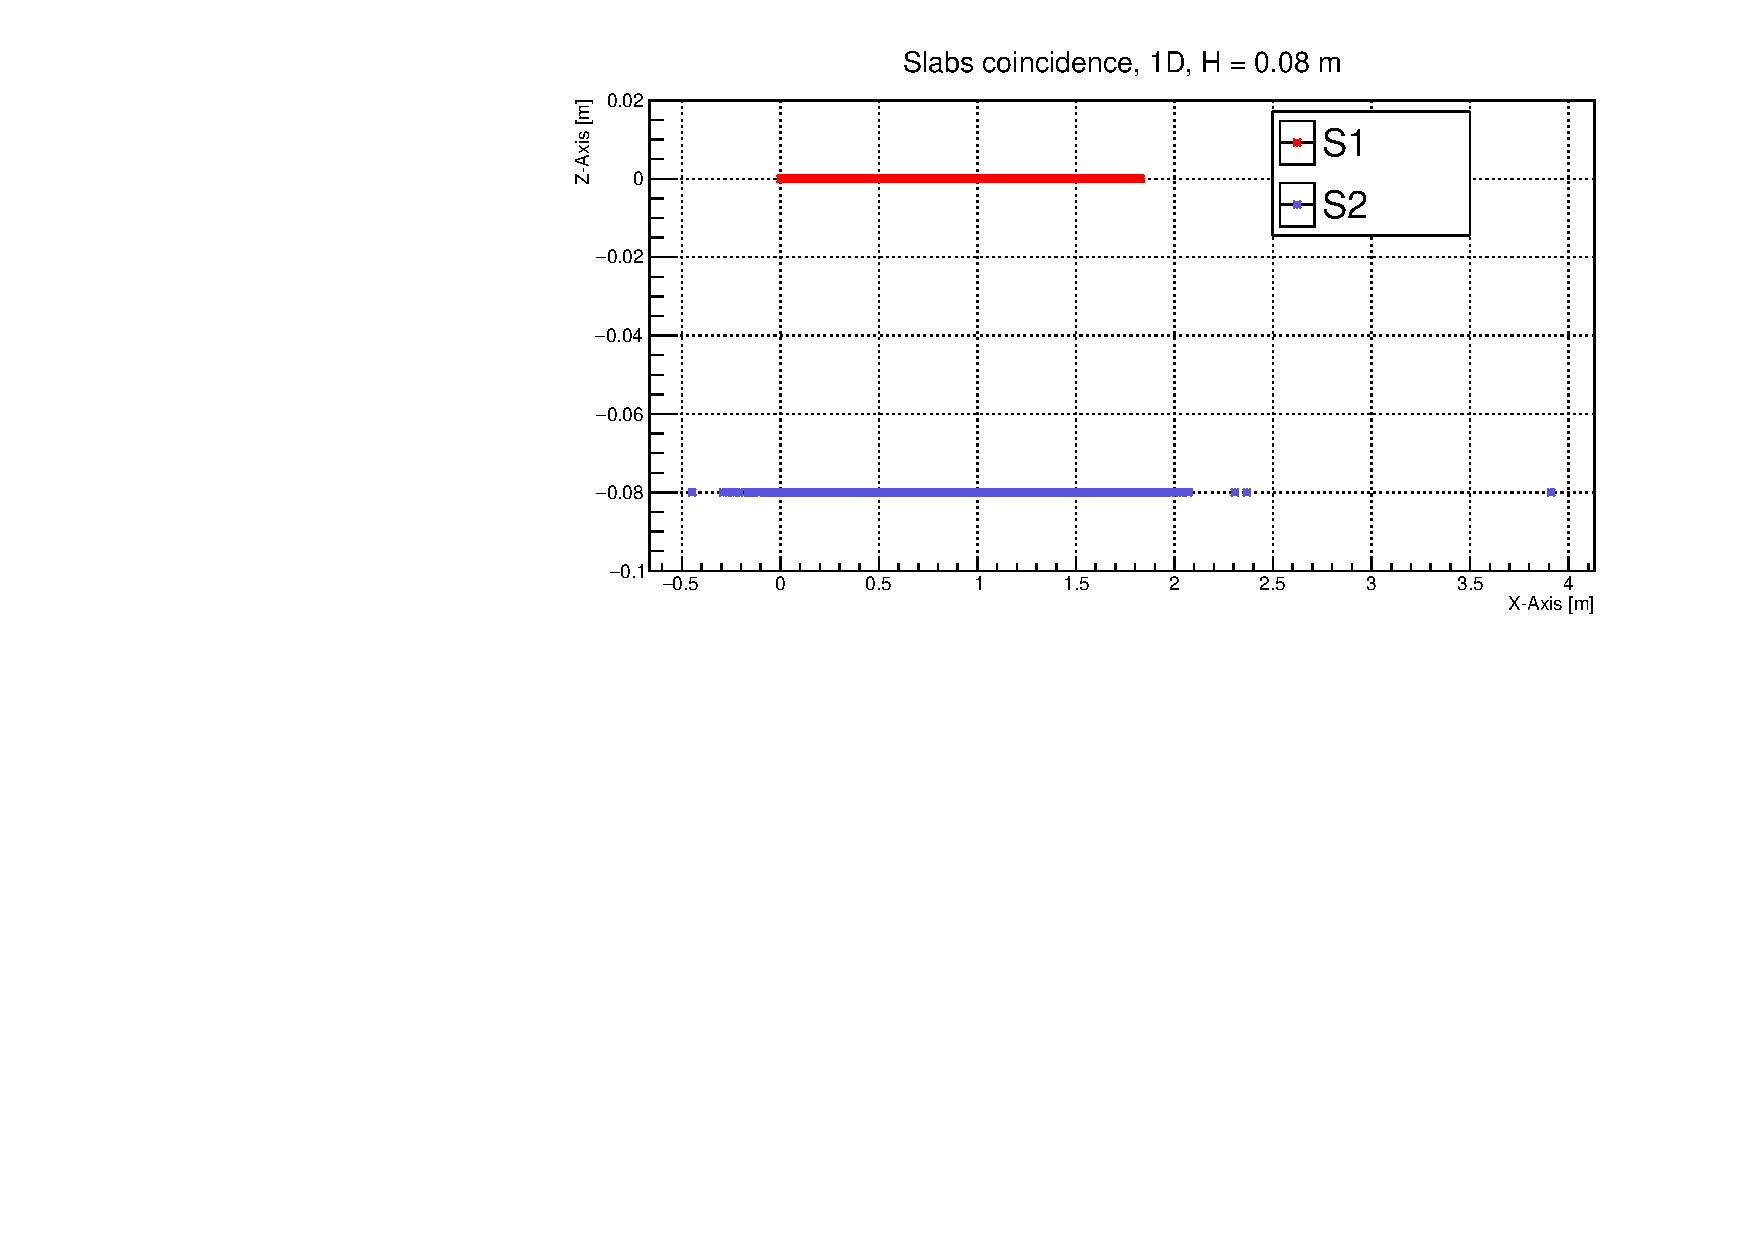
\includegraphics[scale=0.5]{img/1D.pdf}} 
	\subfloat[2D]	
	{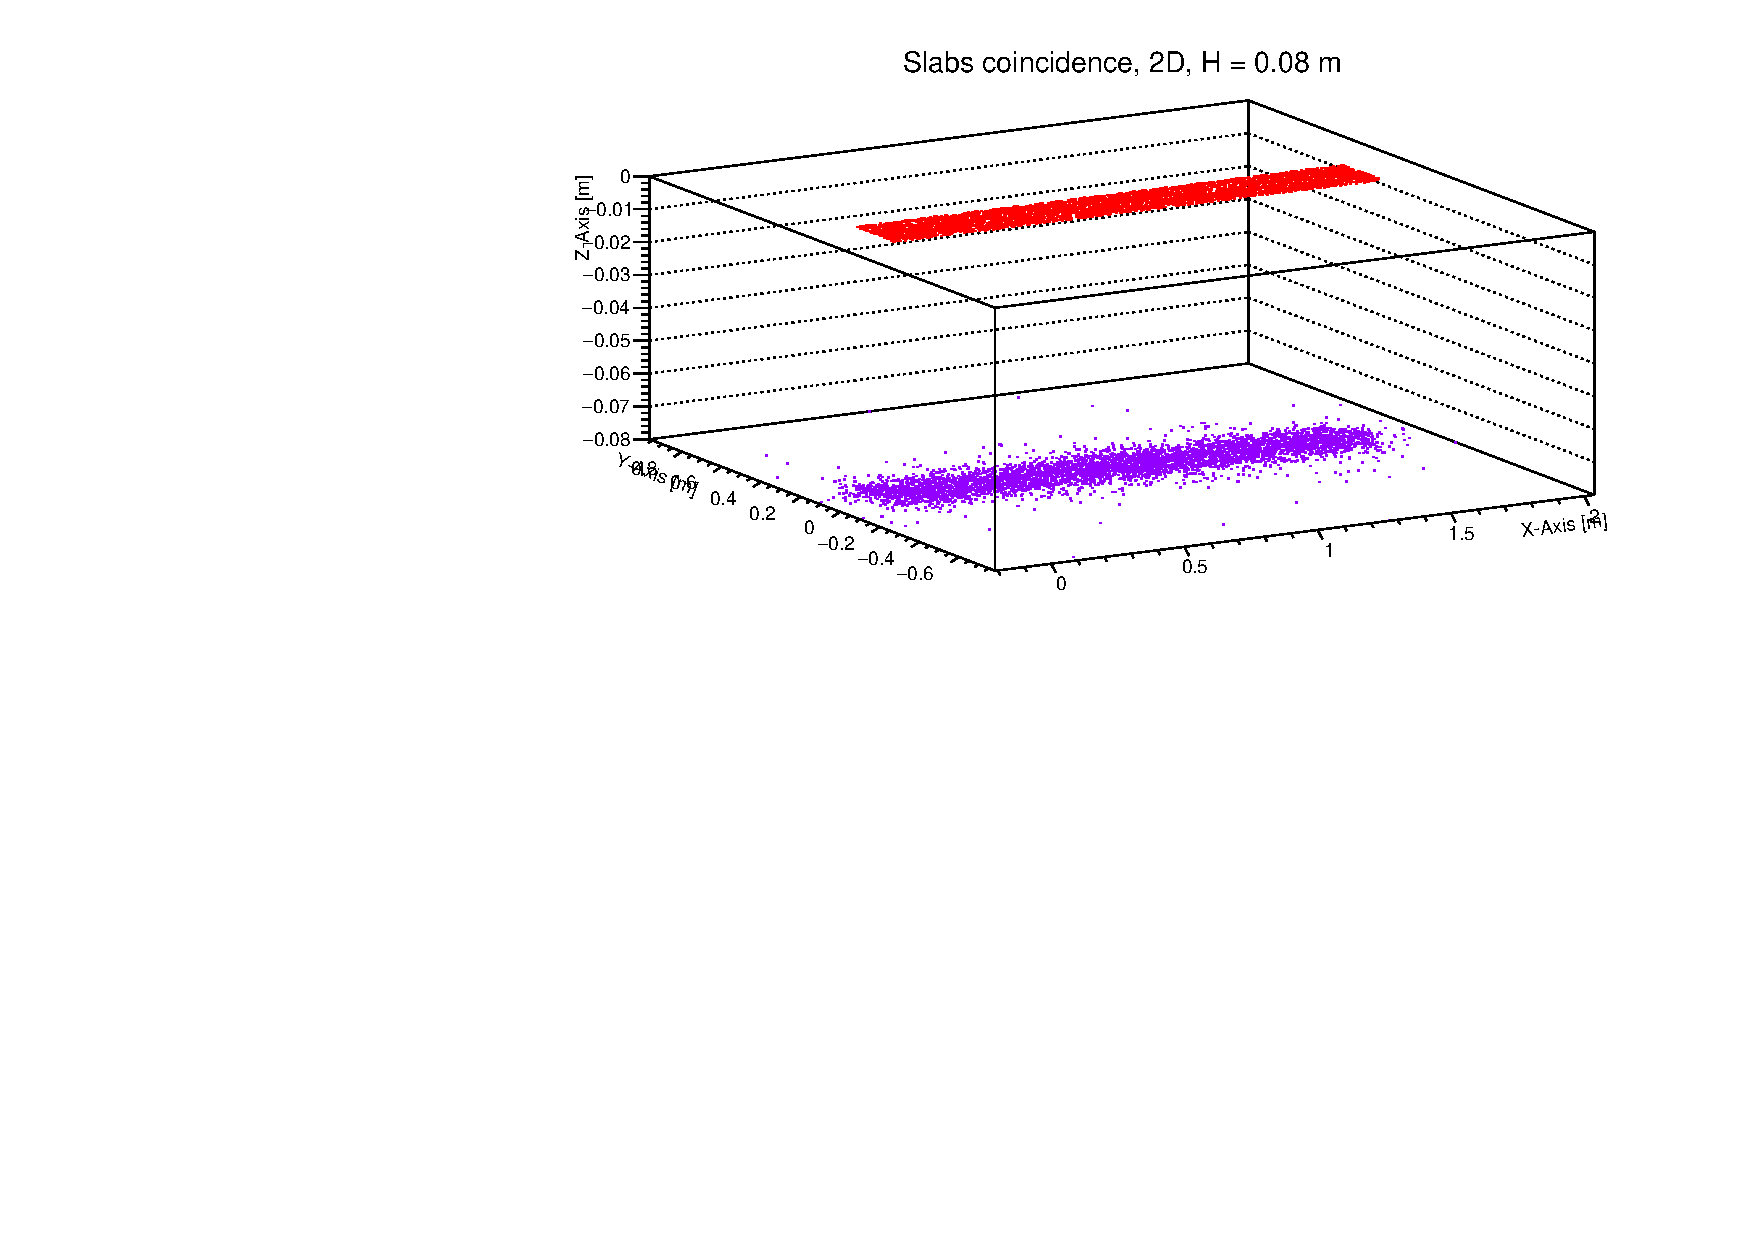
\includegraphics[scale=0.5]{img/2D.pdf}}}
	\centerline{\subfloat[3D]
		{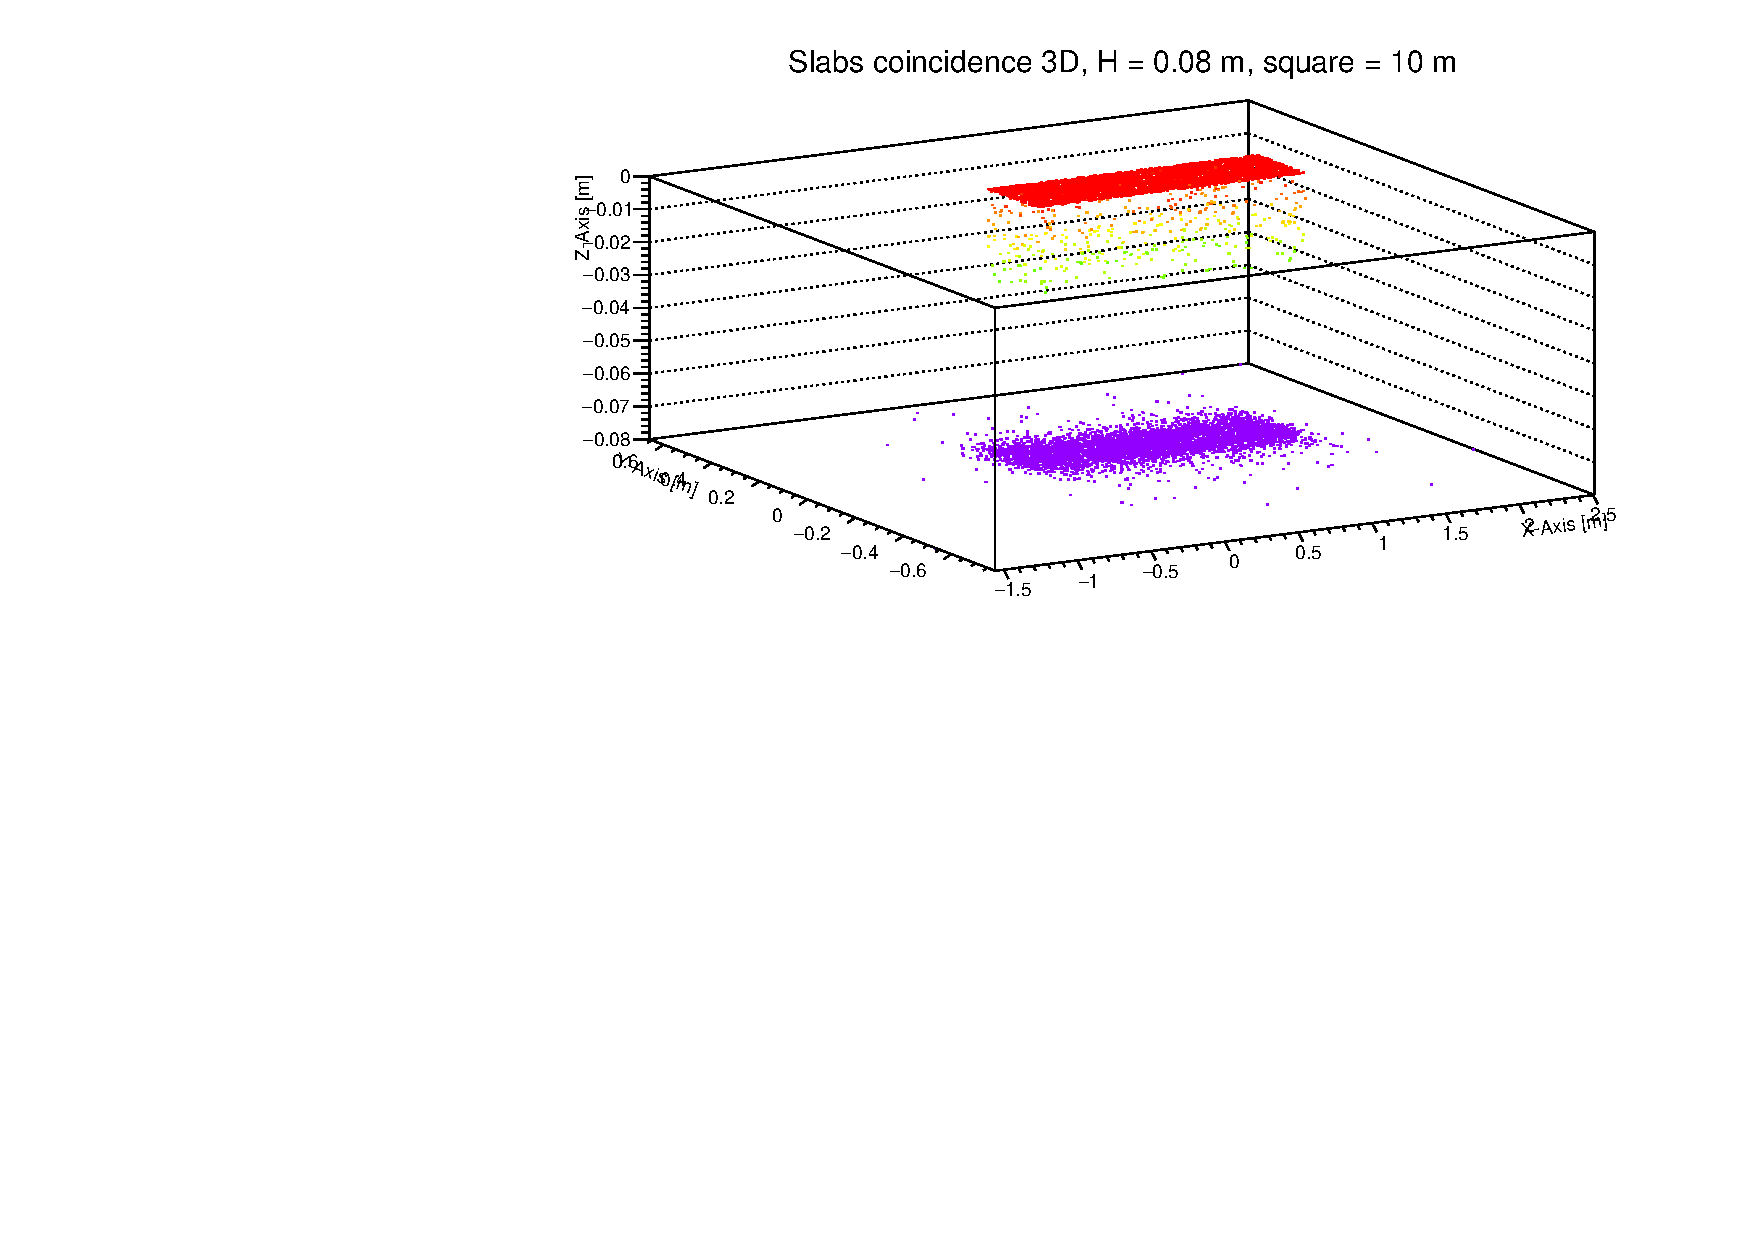
\includegraphics[scale=0.8]{img/3D.pdf}}} 
	\caption{Grafici delle simulazioni.}
	\label{nDsim_plots}
\end{figure}


\section{Grafici}
\vspace{2cm}
\begin{figure}[h]
	\centerline{\subfloat[Nr.~437]
		{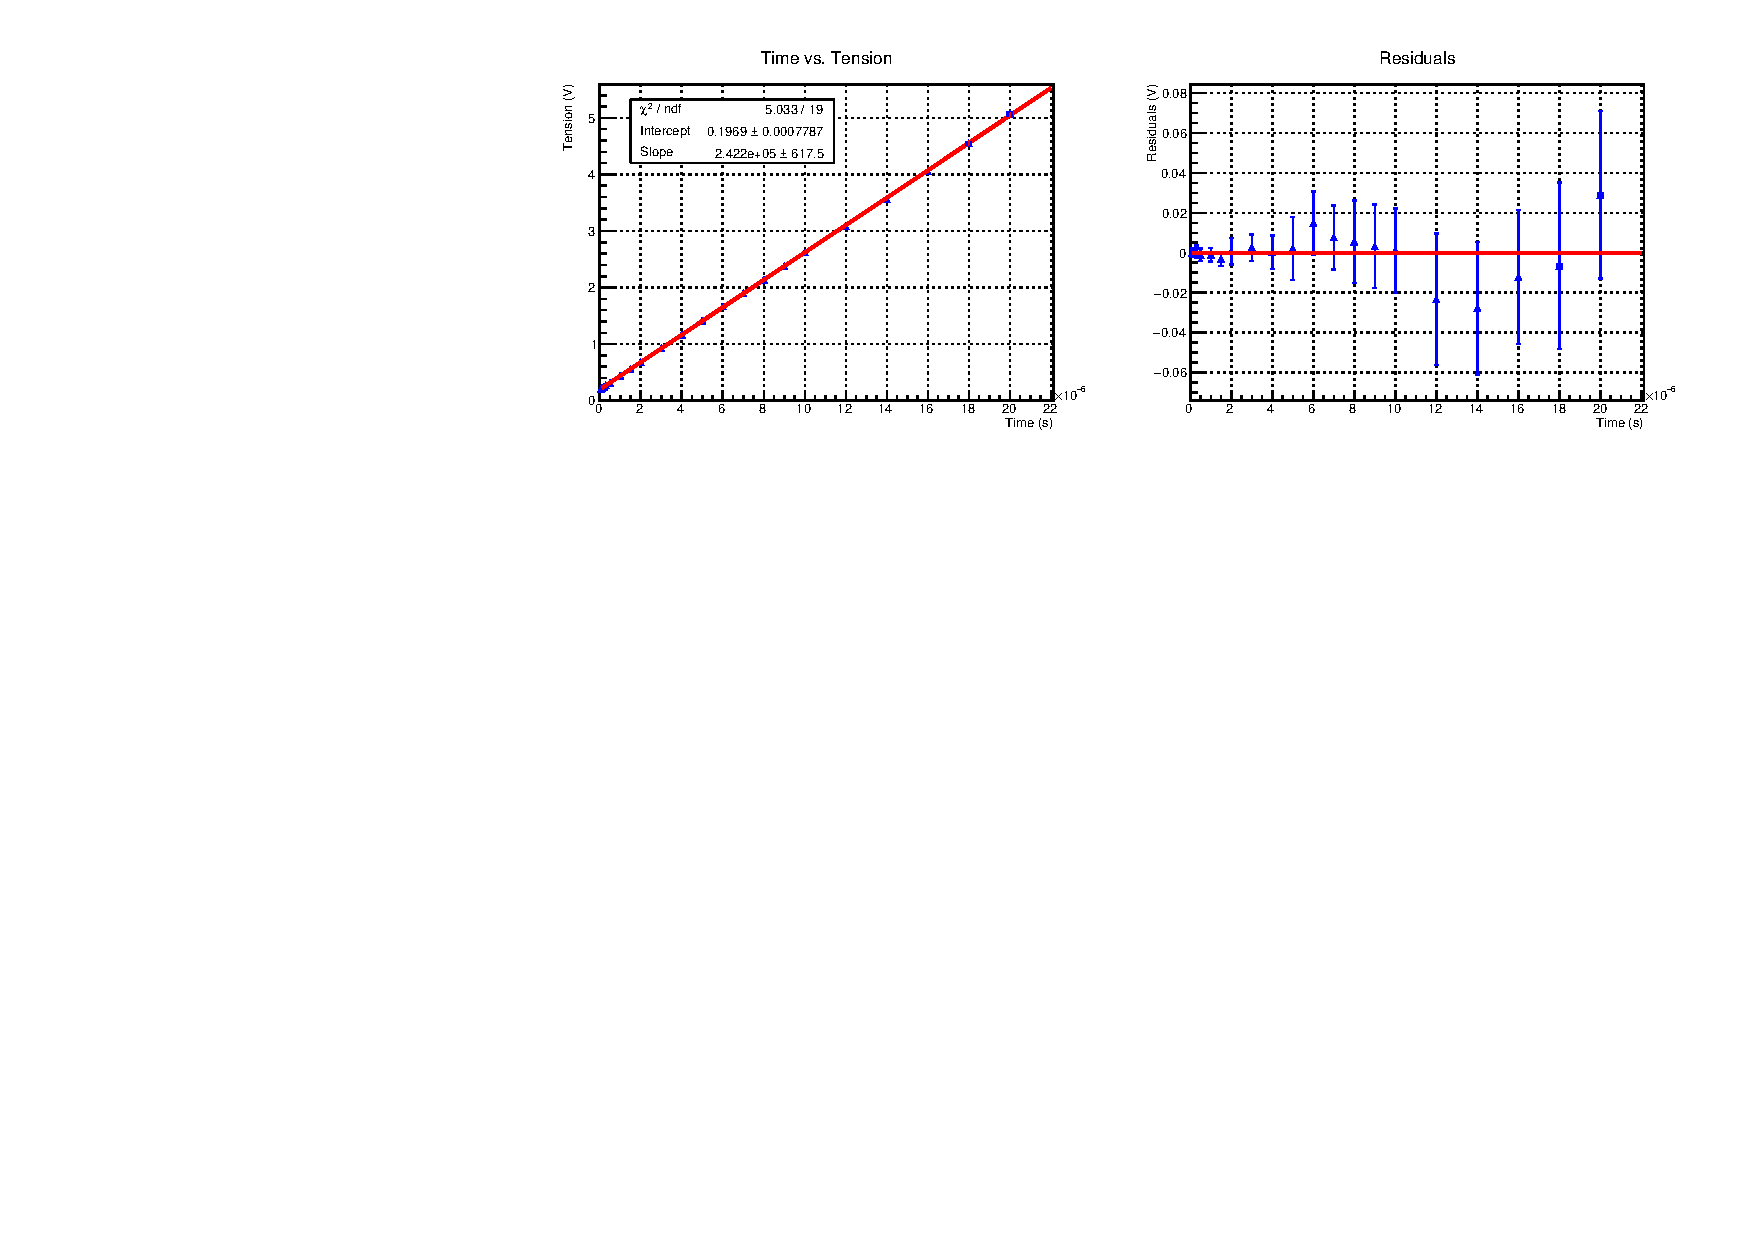
\includegraphics[scale=1.0]{img/time_tens_437.pdf}}}
	\centerline{\subfloat[Nr.~467]
		{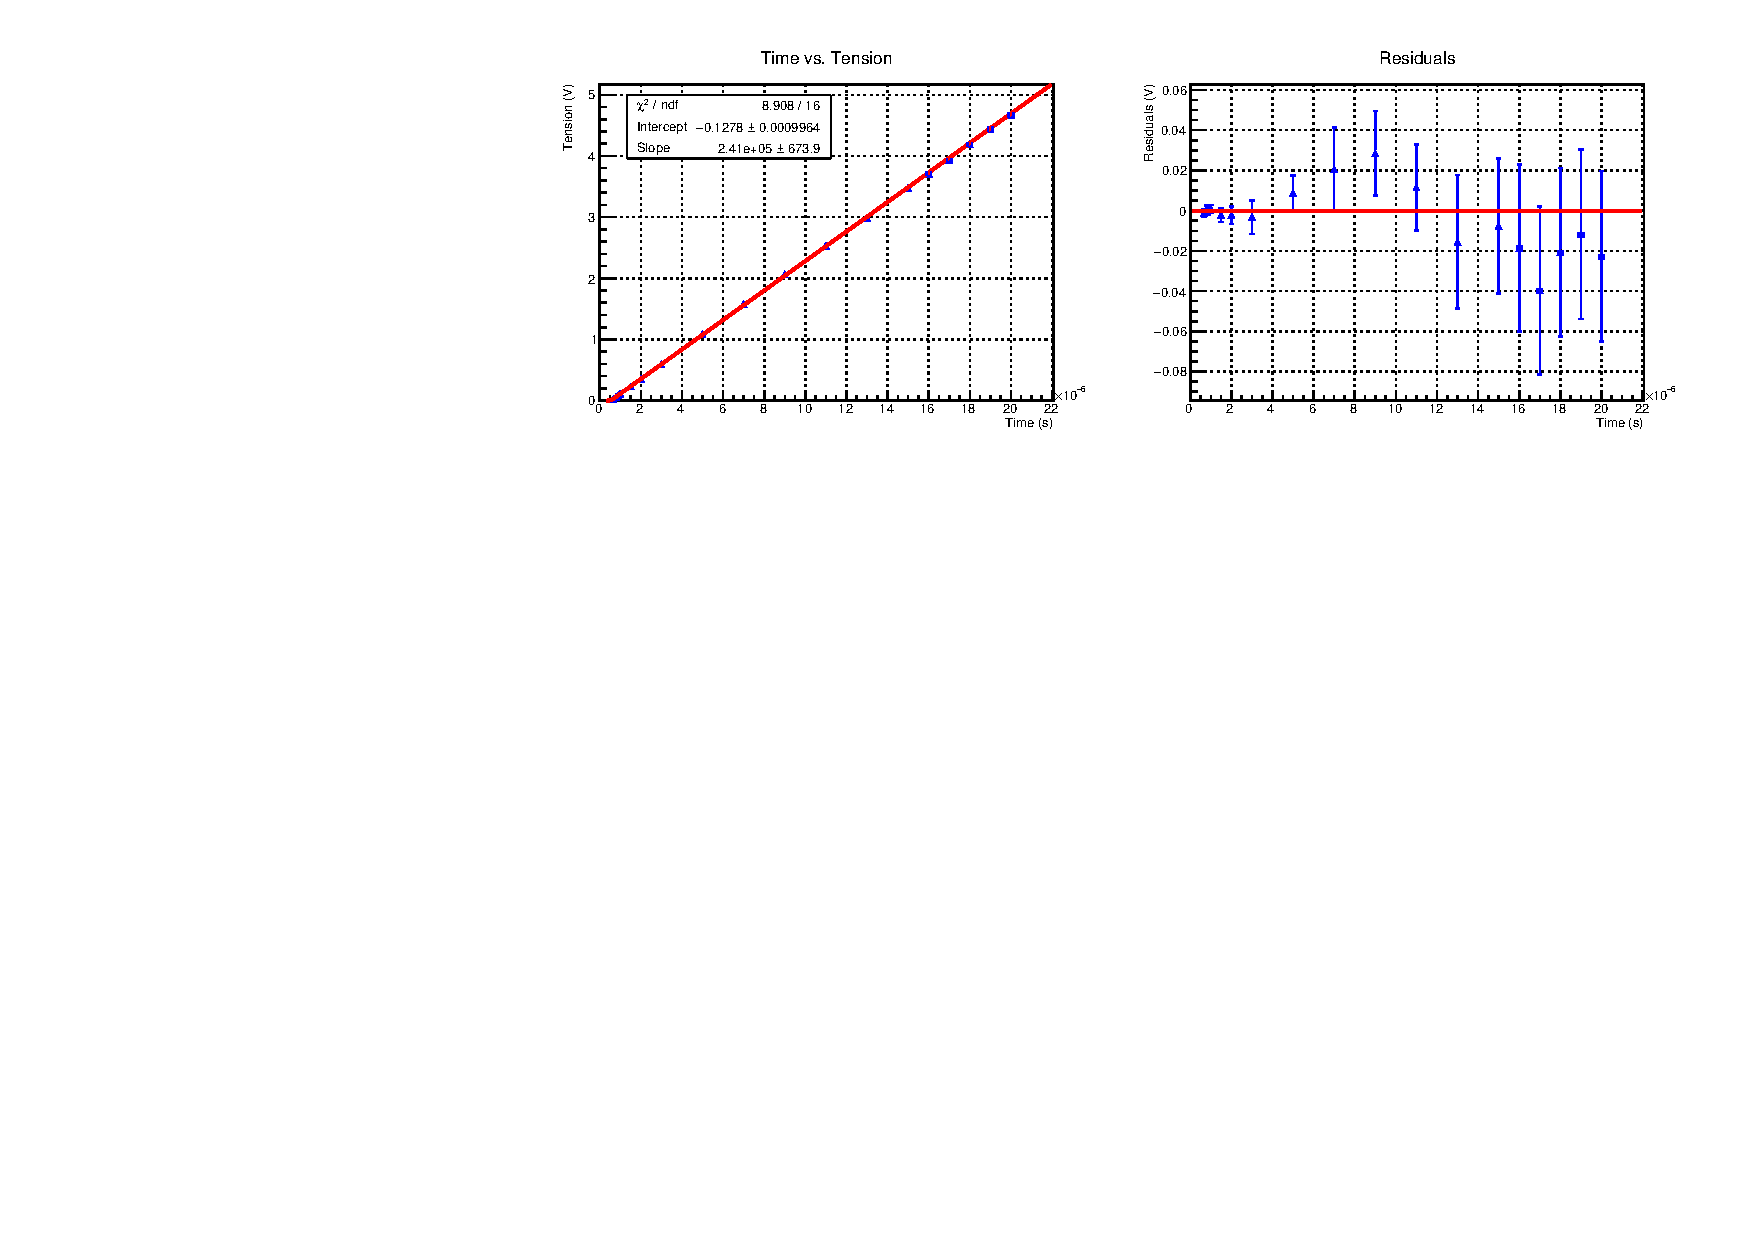
\includegraphics[scale=1.0]{img/time_tens_467.pdf}}} 
	\caption{Valori di tensione erogati in base al ritardo.}
	\label{time_tens}
\end{figure}
\begin{figure}[h]
	\centerline{\subfloat[Nr.~437]
		{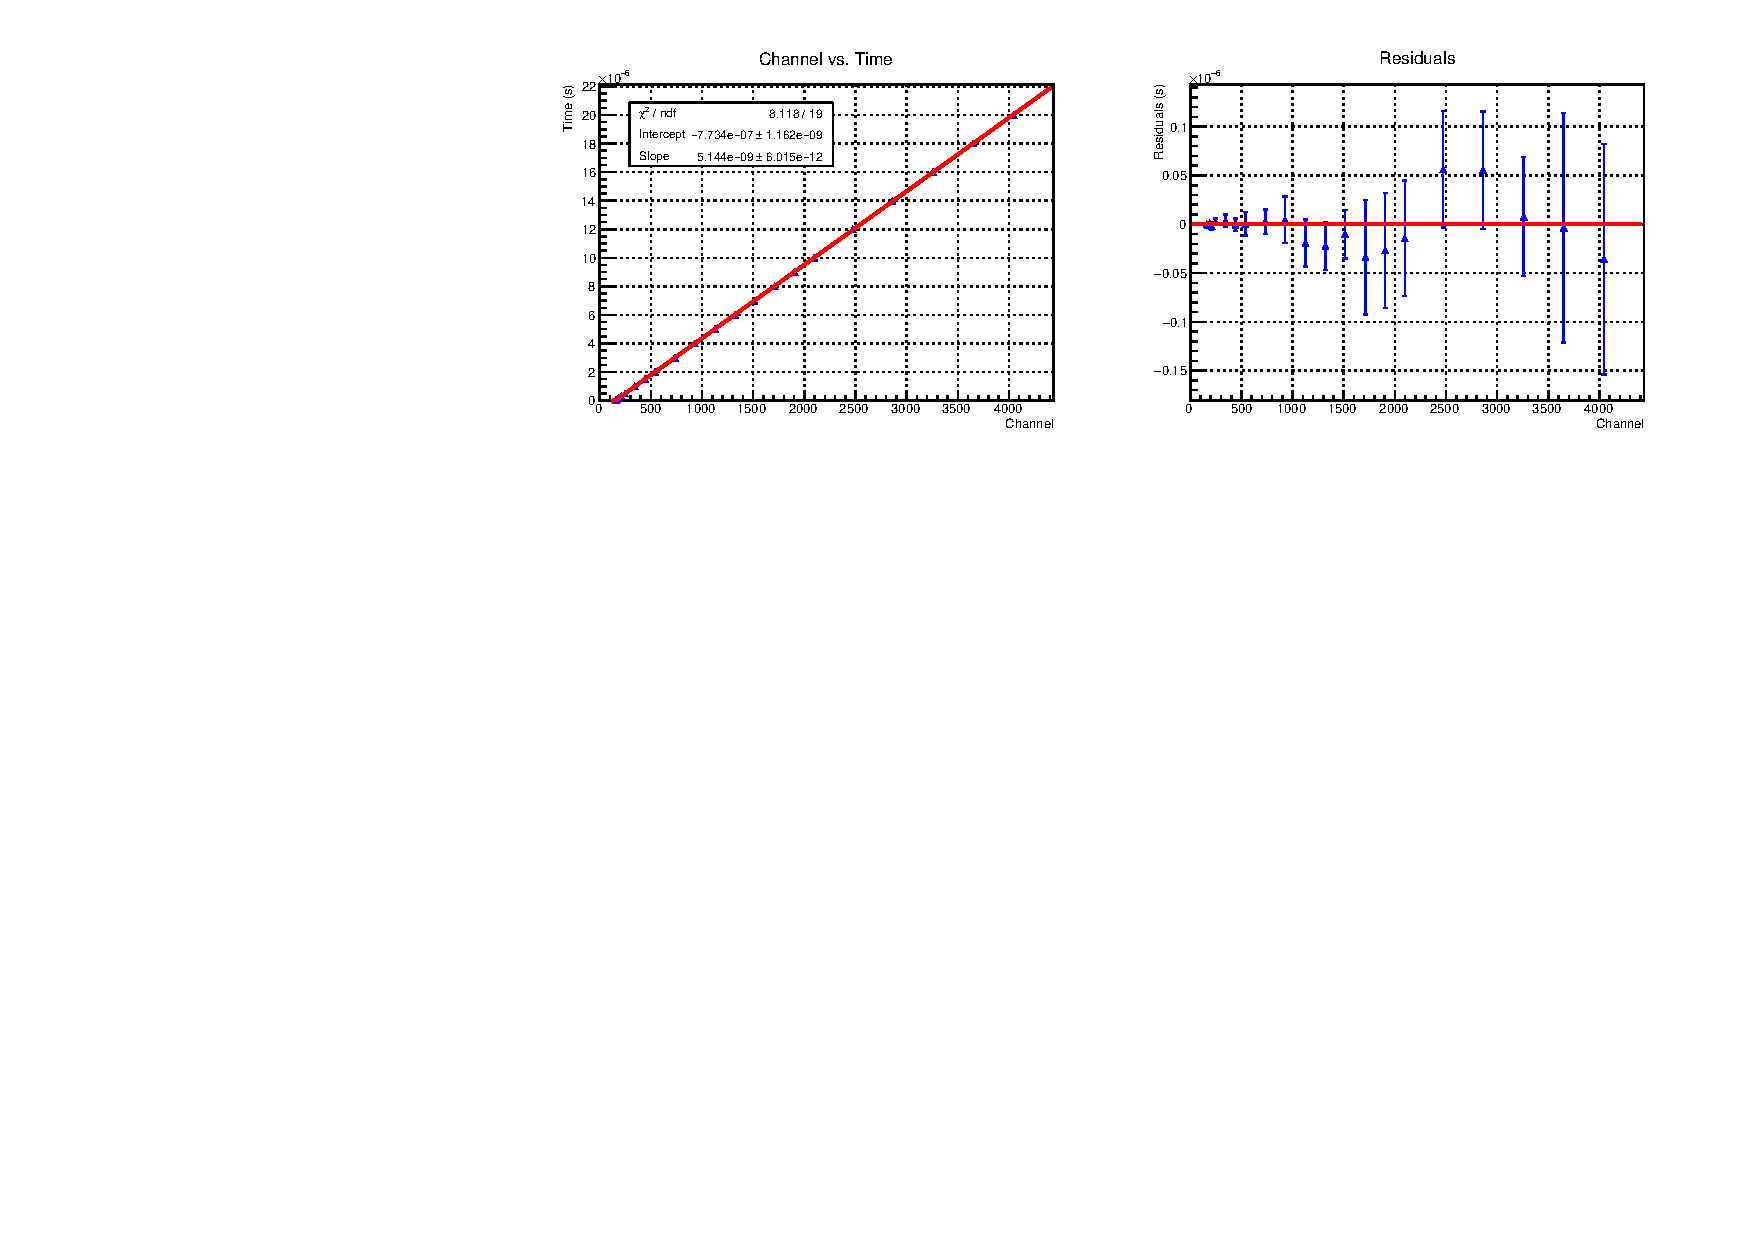
\includegraphics[scale=1.0]{img/chan_time_437.pdf}}}
	\centerline{\subfloat[Nr.~467]
		{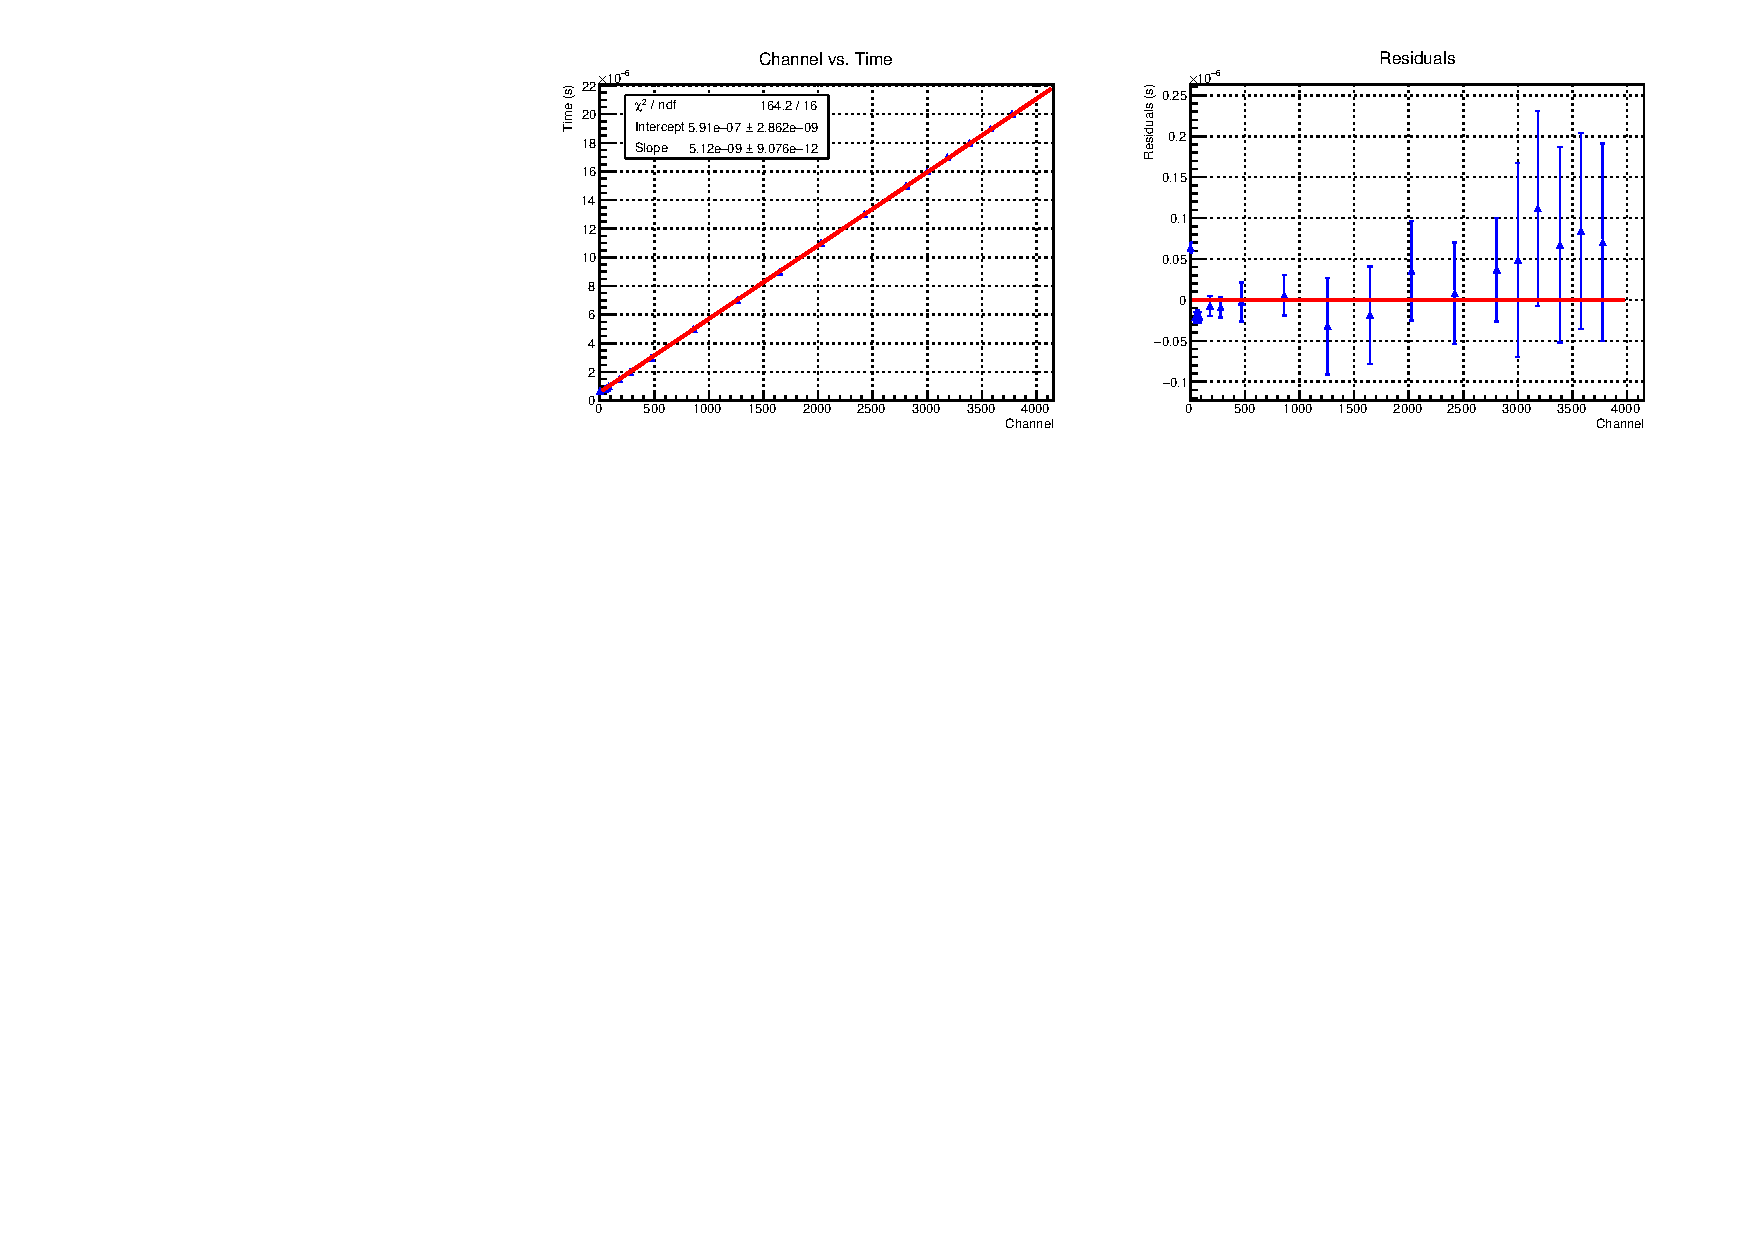
\includegraphics[scale=1.0]{img/chan_time_467.pdf}}}
	\caption{Canali corrispondenti ai ritardi impostati.}
	\label{chan_time}
\end{figure}
\begin{figure}[h]
	\centerline{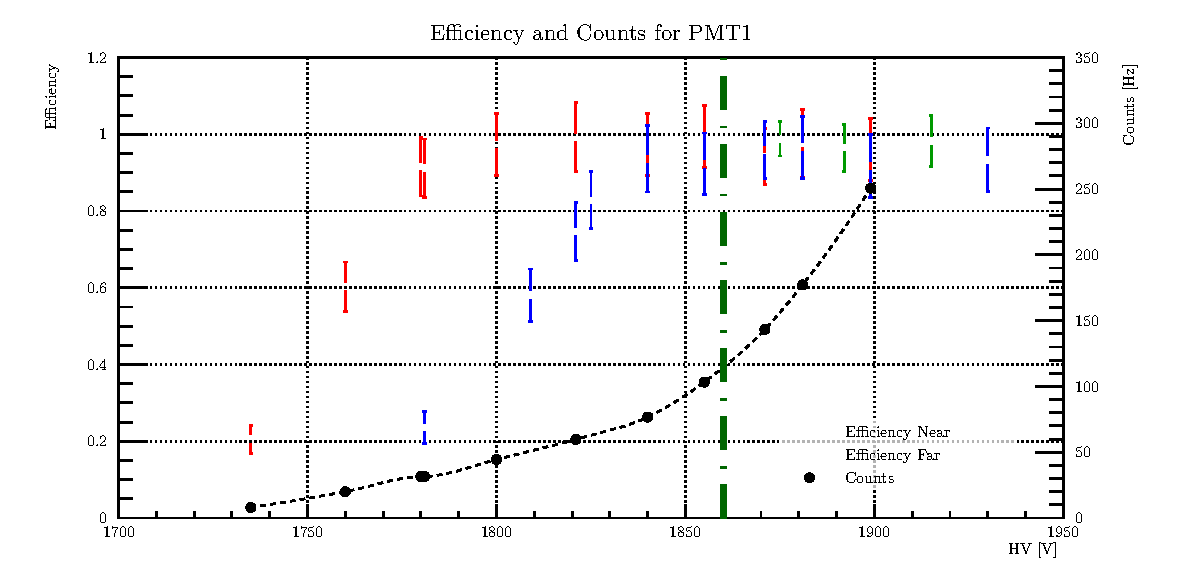
\includegraphics[scale=0.8]{img/eff1.pdf}}
\end{figure}
\begin{figure}[h]
	\centerline{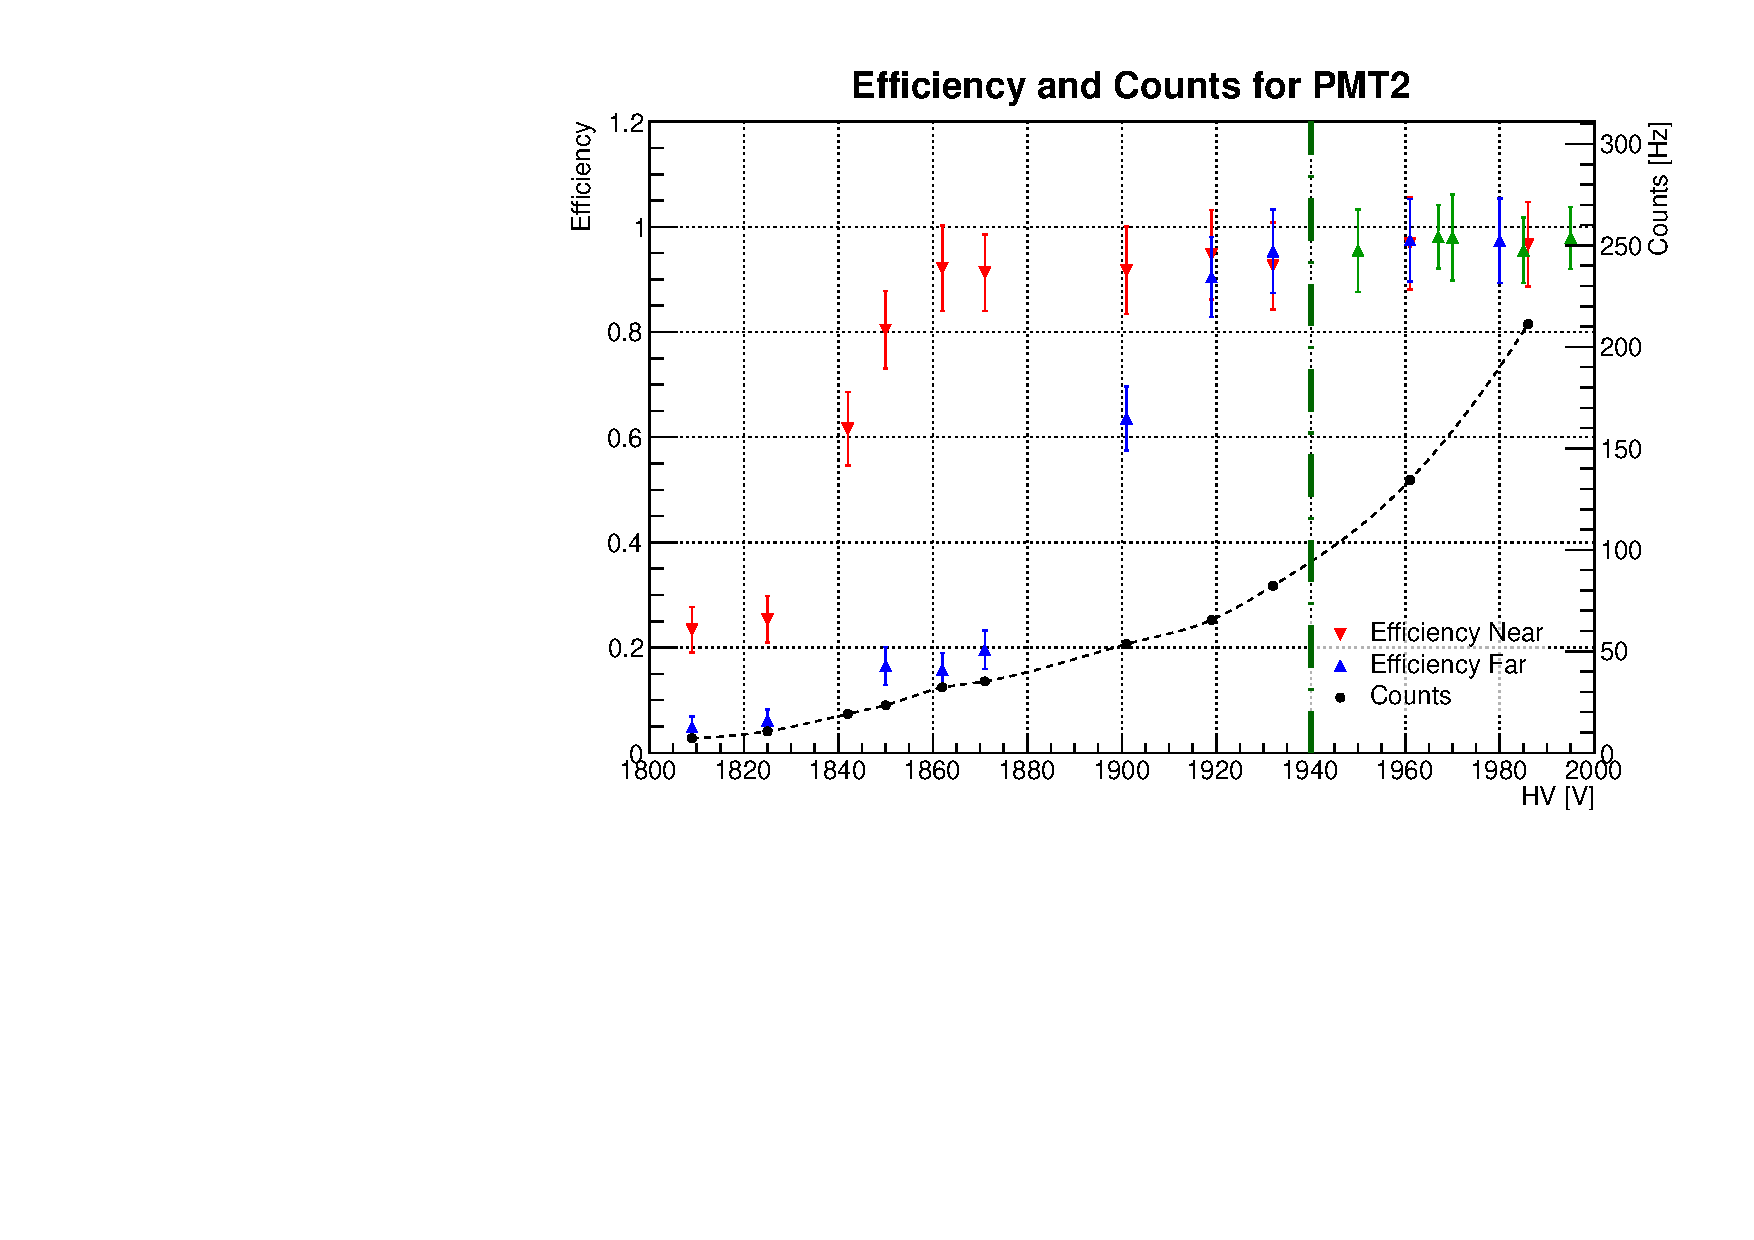
\includegraphics[scale=0.8]{img/eff2.pdf}}	
\end{figure}
\begin{figure}[h]
	\centerline{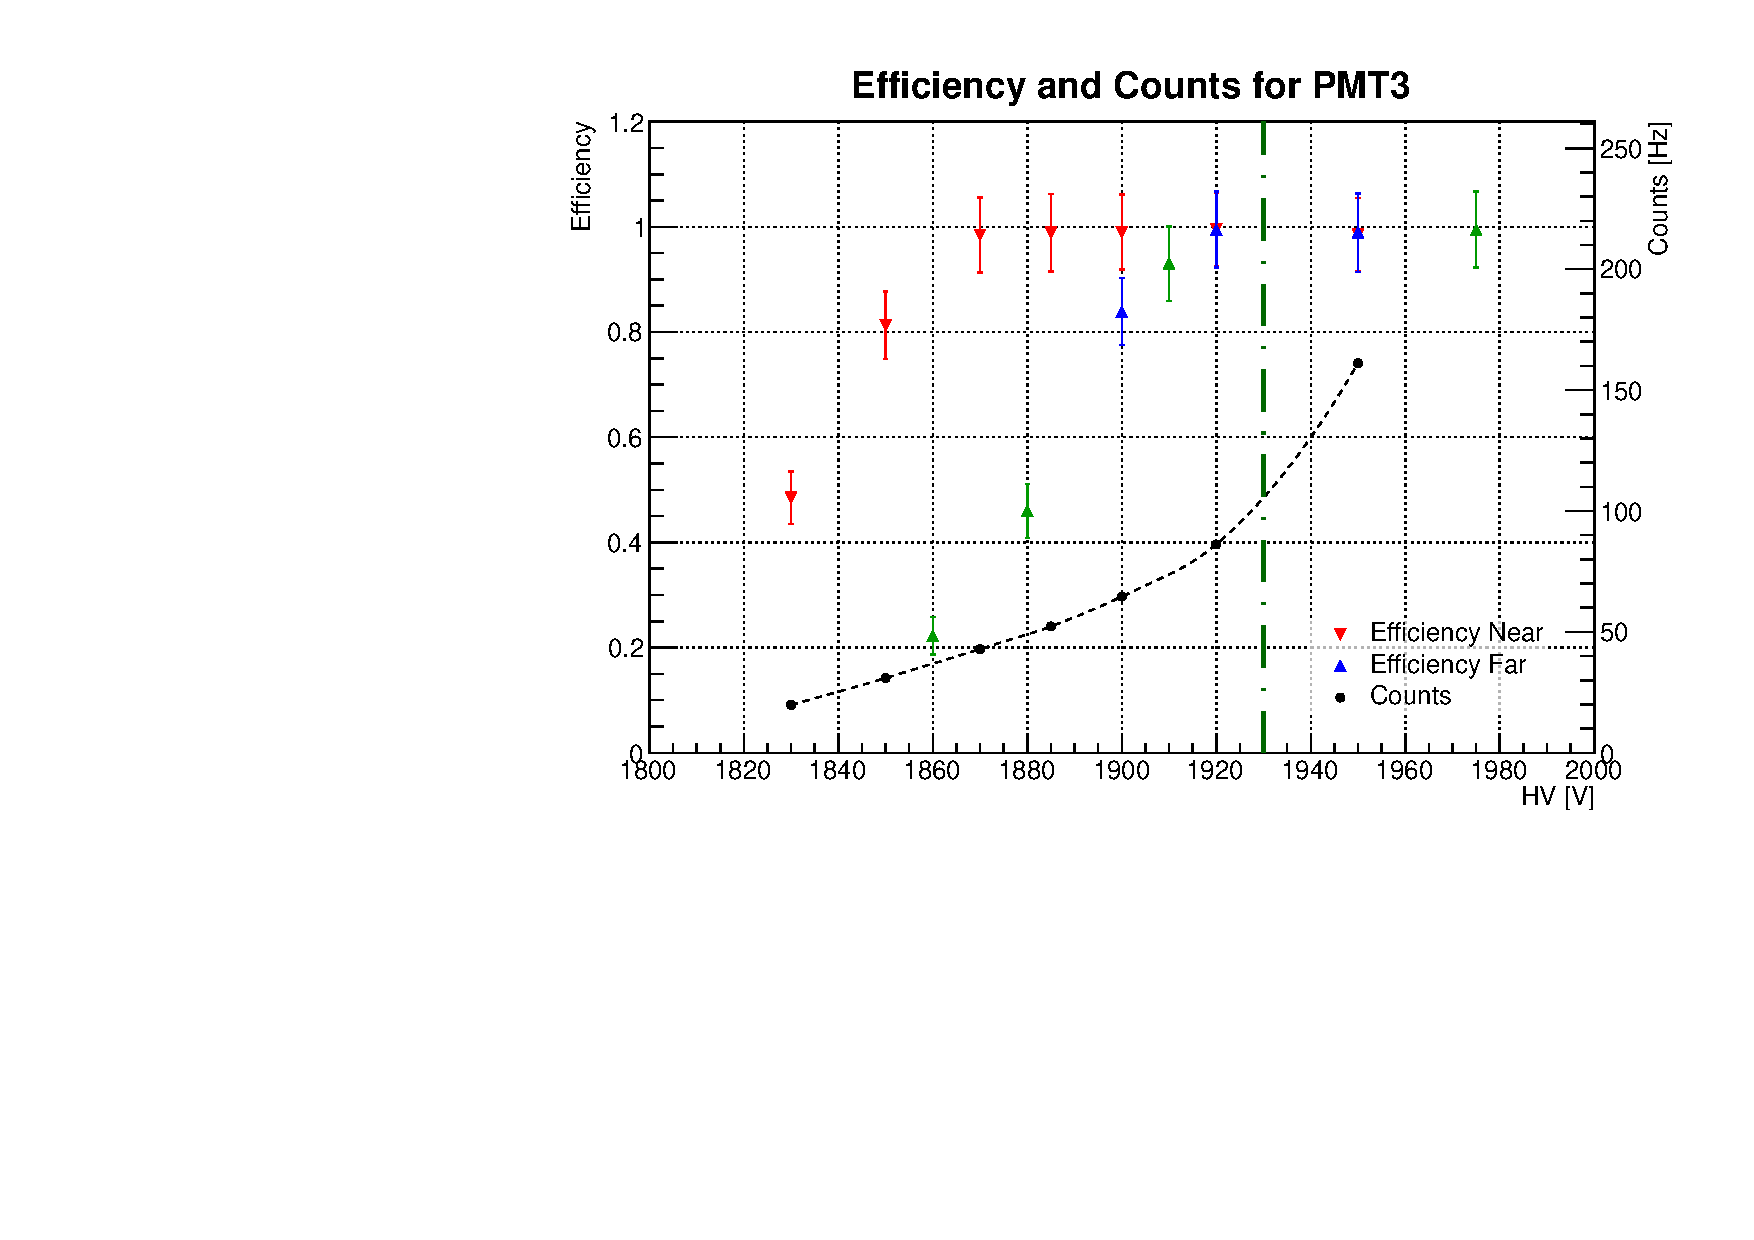
\includegraphics[scale=0.8]{img/eff3.pdf}}	
\end{figure}
\begin{figure}[h]
	\centerline{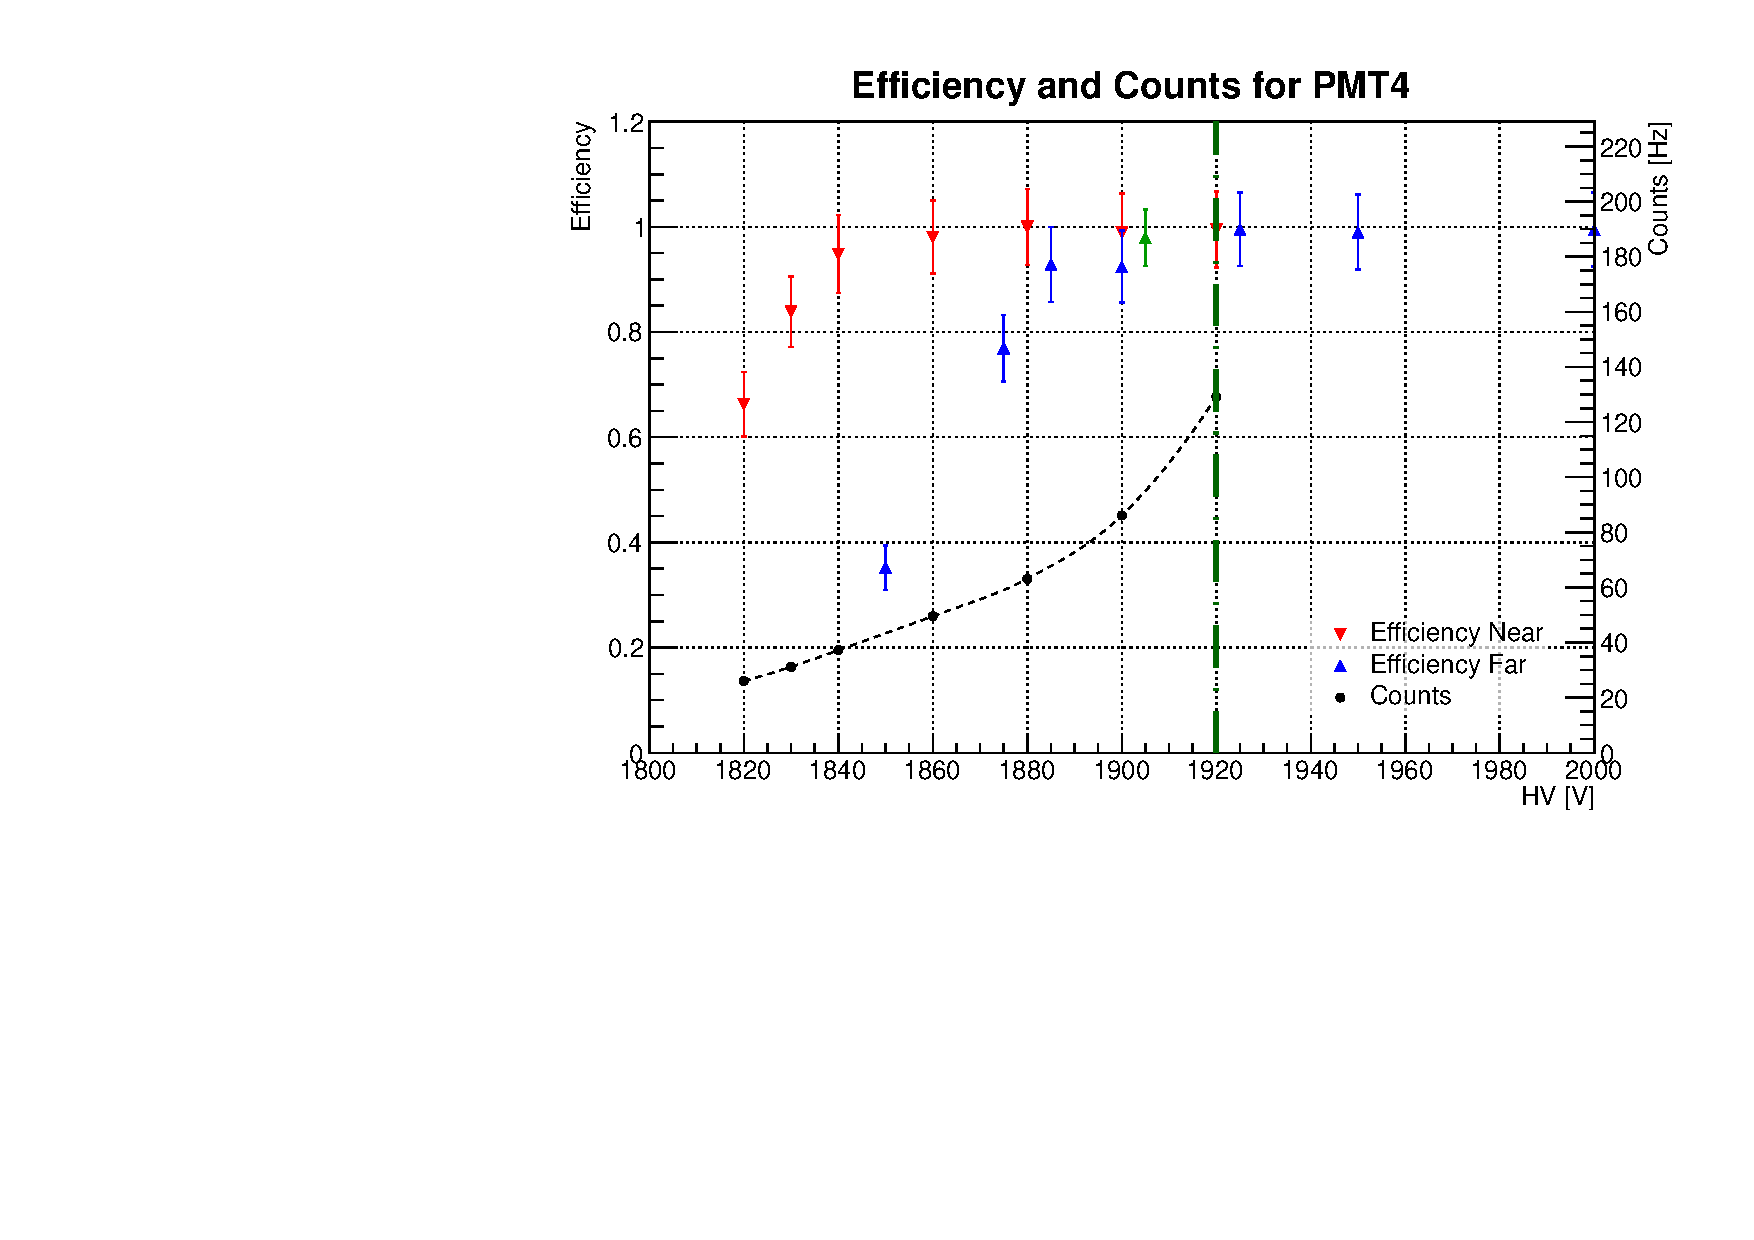
\includegraphics[scale=0.8]{img/eff4.pdf}}
\end{figure}
\begin{figure}[h]
	\centerline{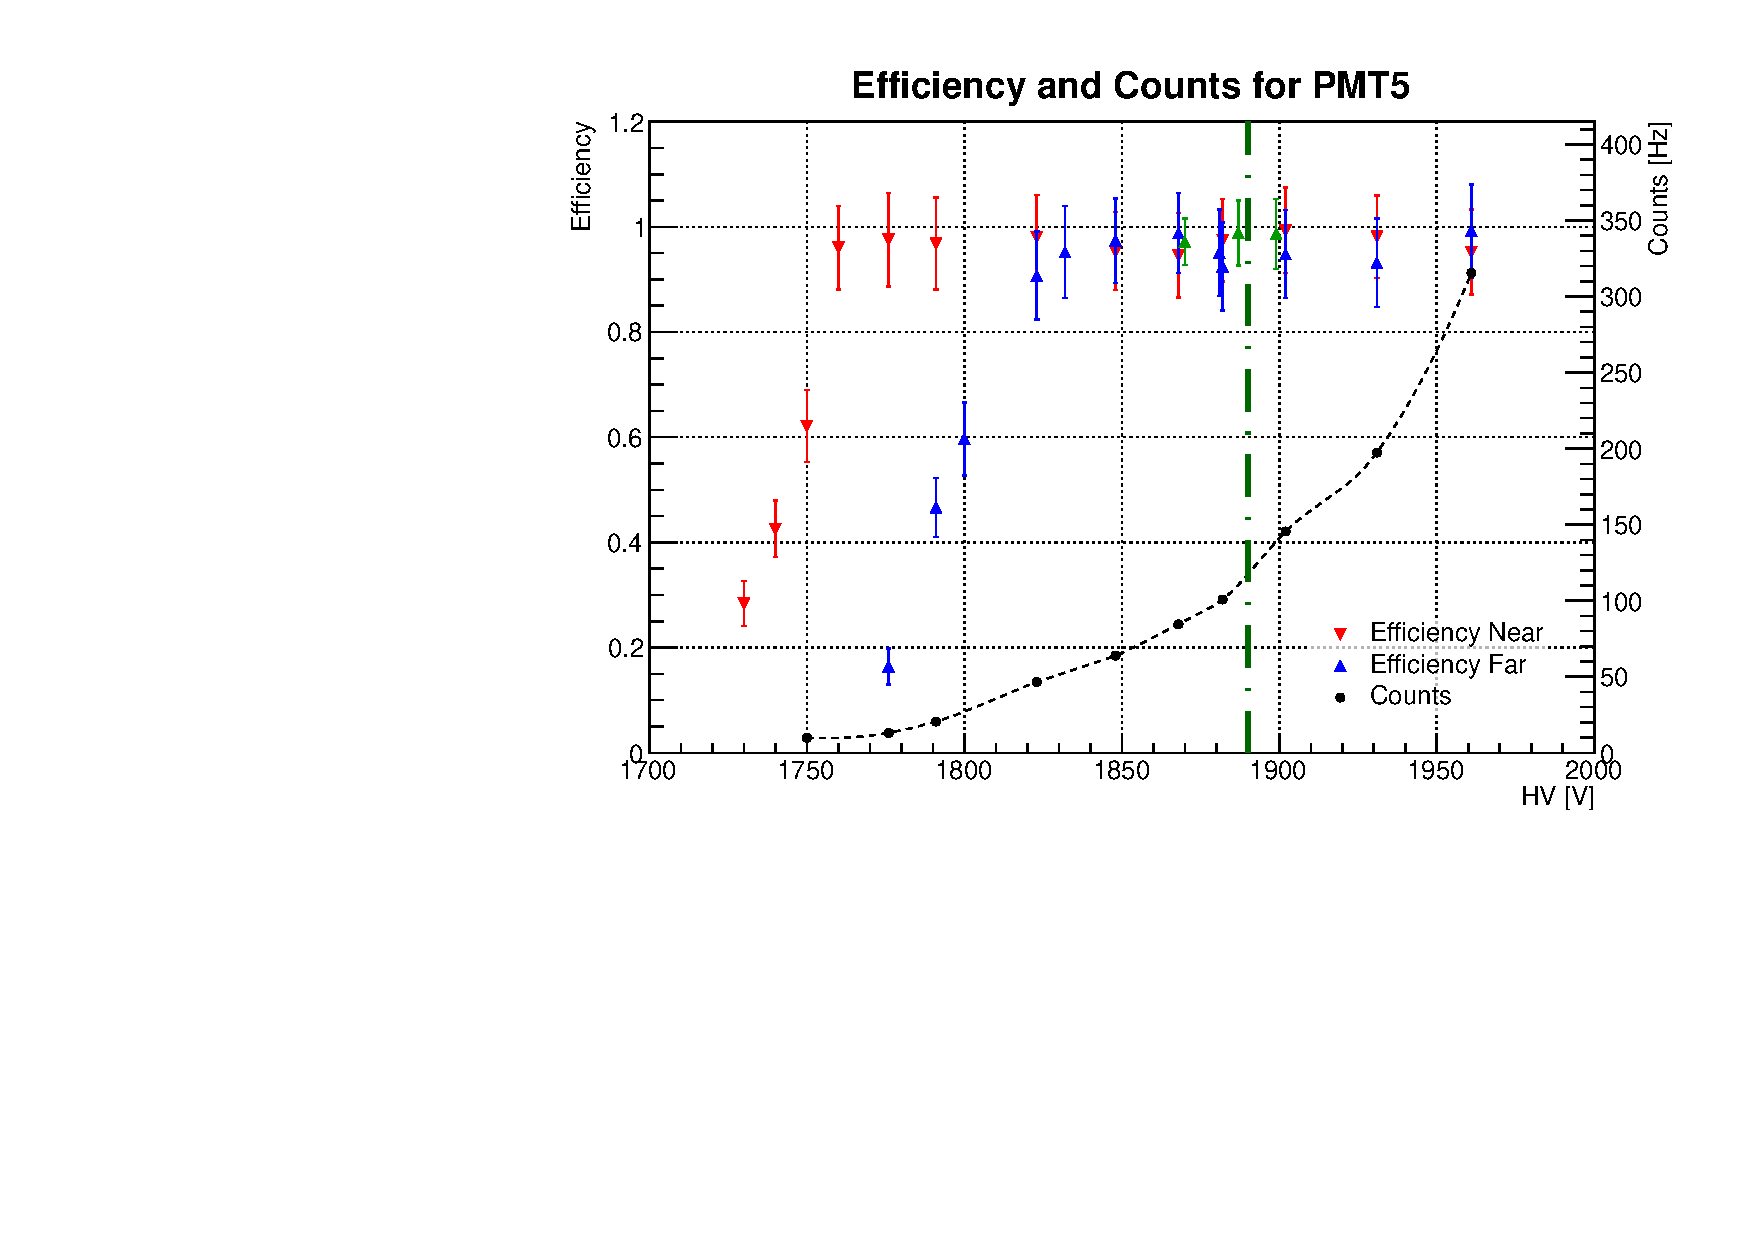
\includegraphics[scale=0.8]{img/eff5.pdf}}
\end{figure}
\begin{figure}[h]
	\centerline{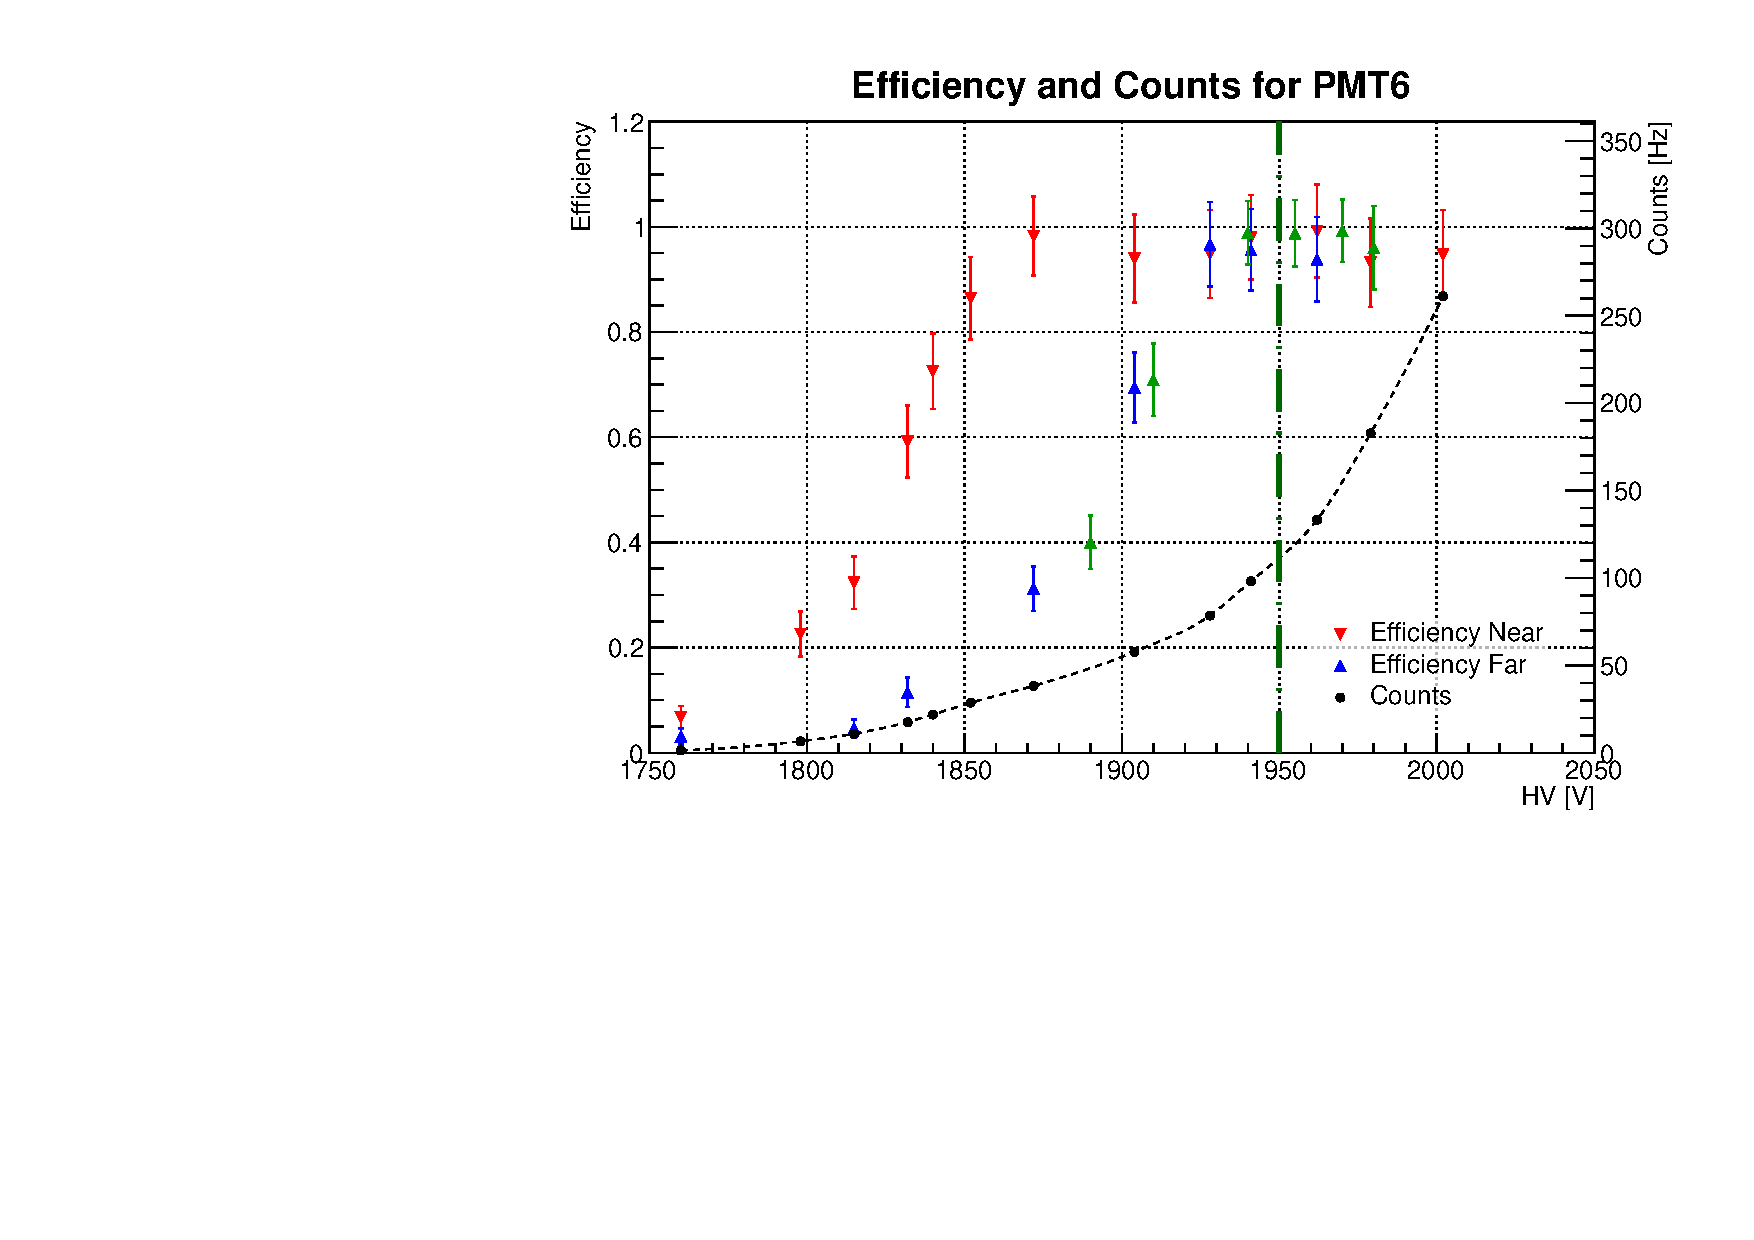
\includegraphics[scale=0.8]{img/eff6.pdf}}
\end{figure}
\begin{figure}[h]
	\centerline{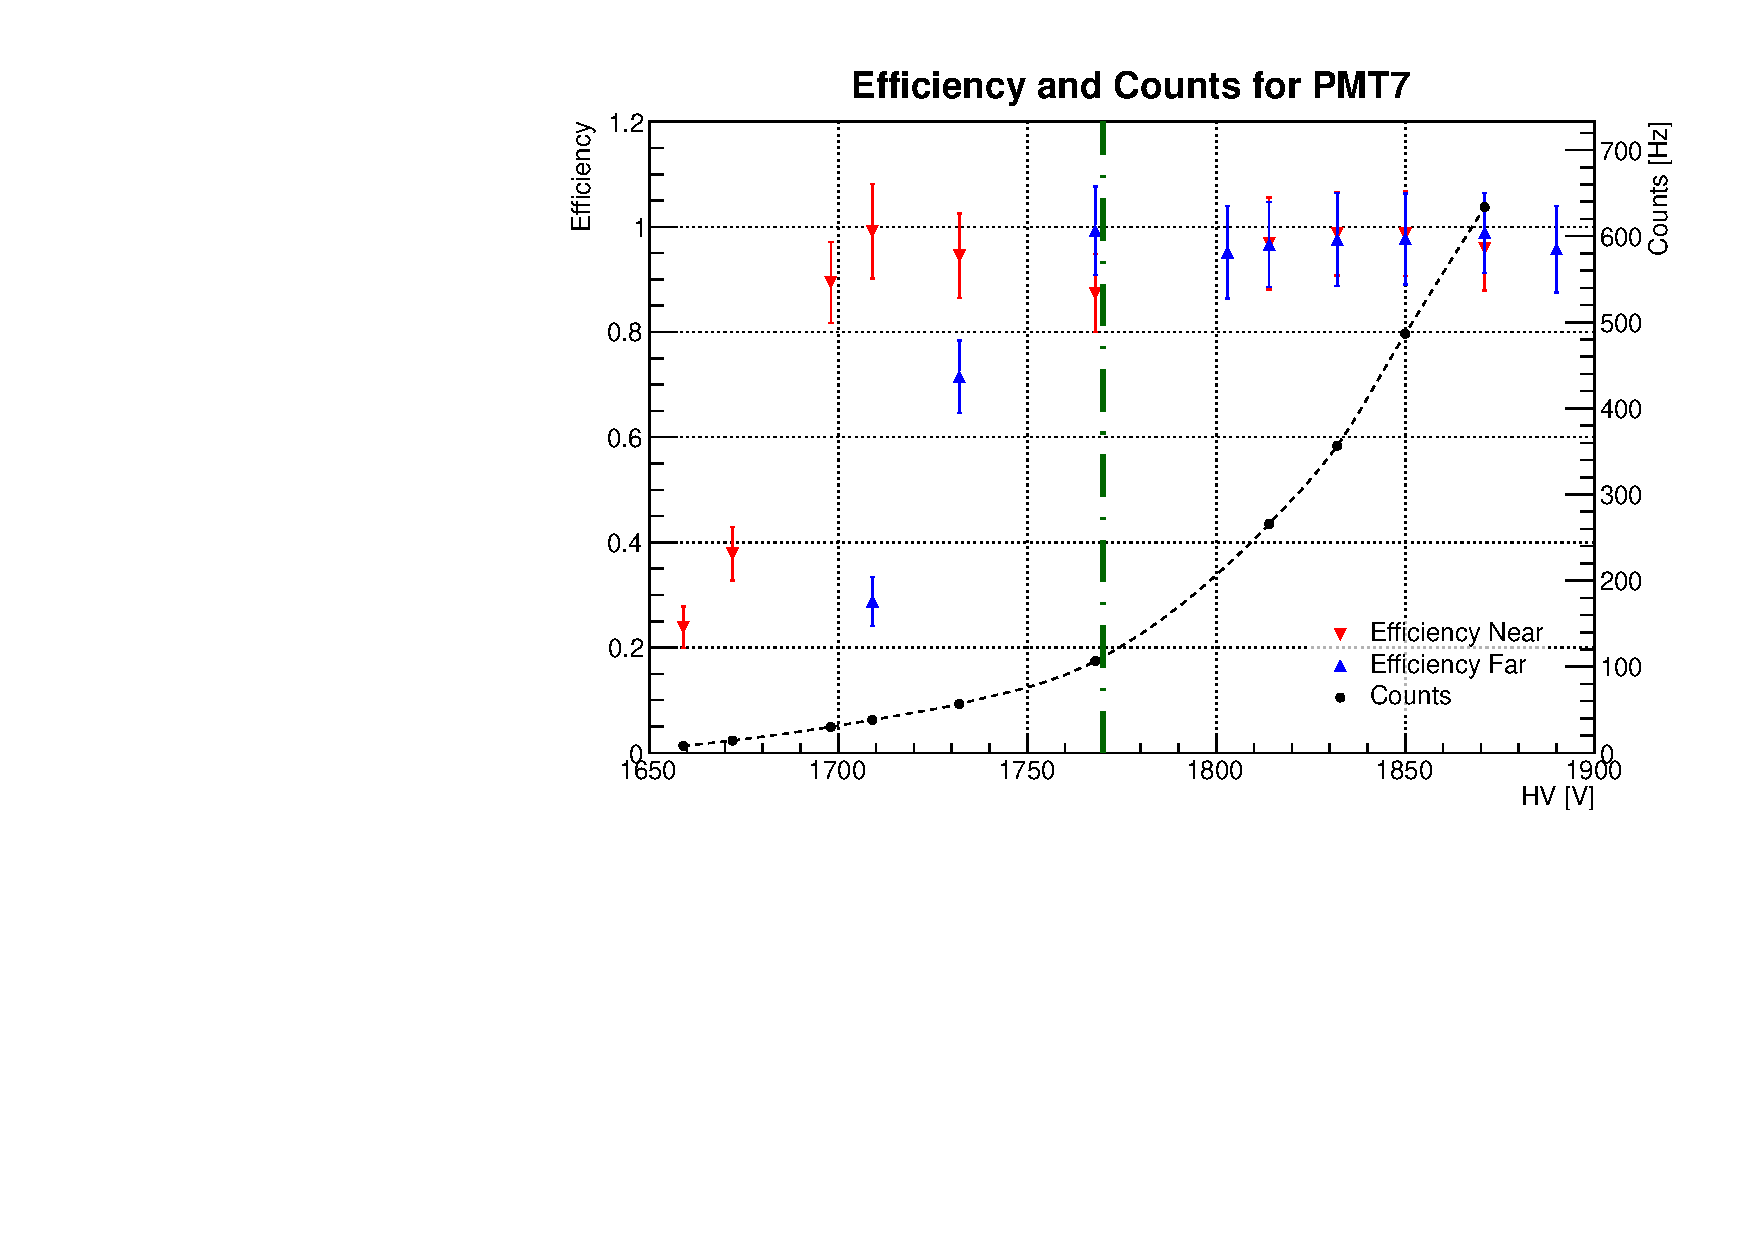
\includegraphics[scale=0.8]{img/eff7.pdf}}
\end{figure}
\begin{figure}[h]
	\centerline{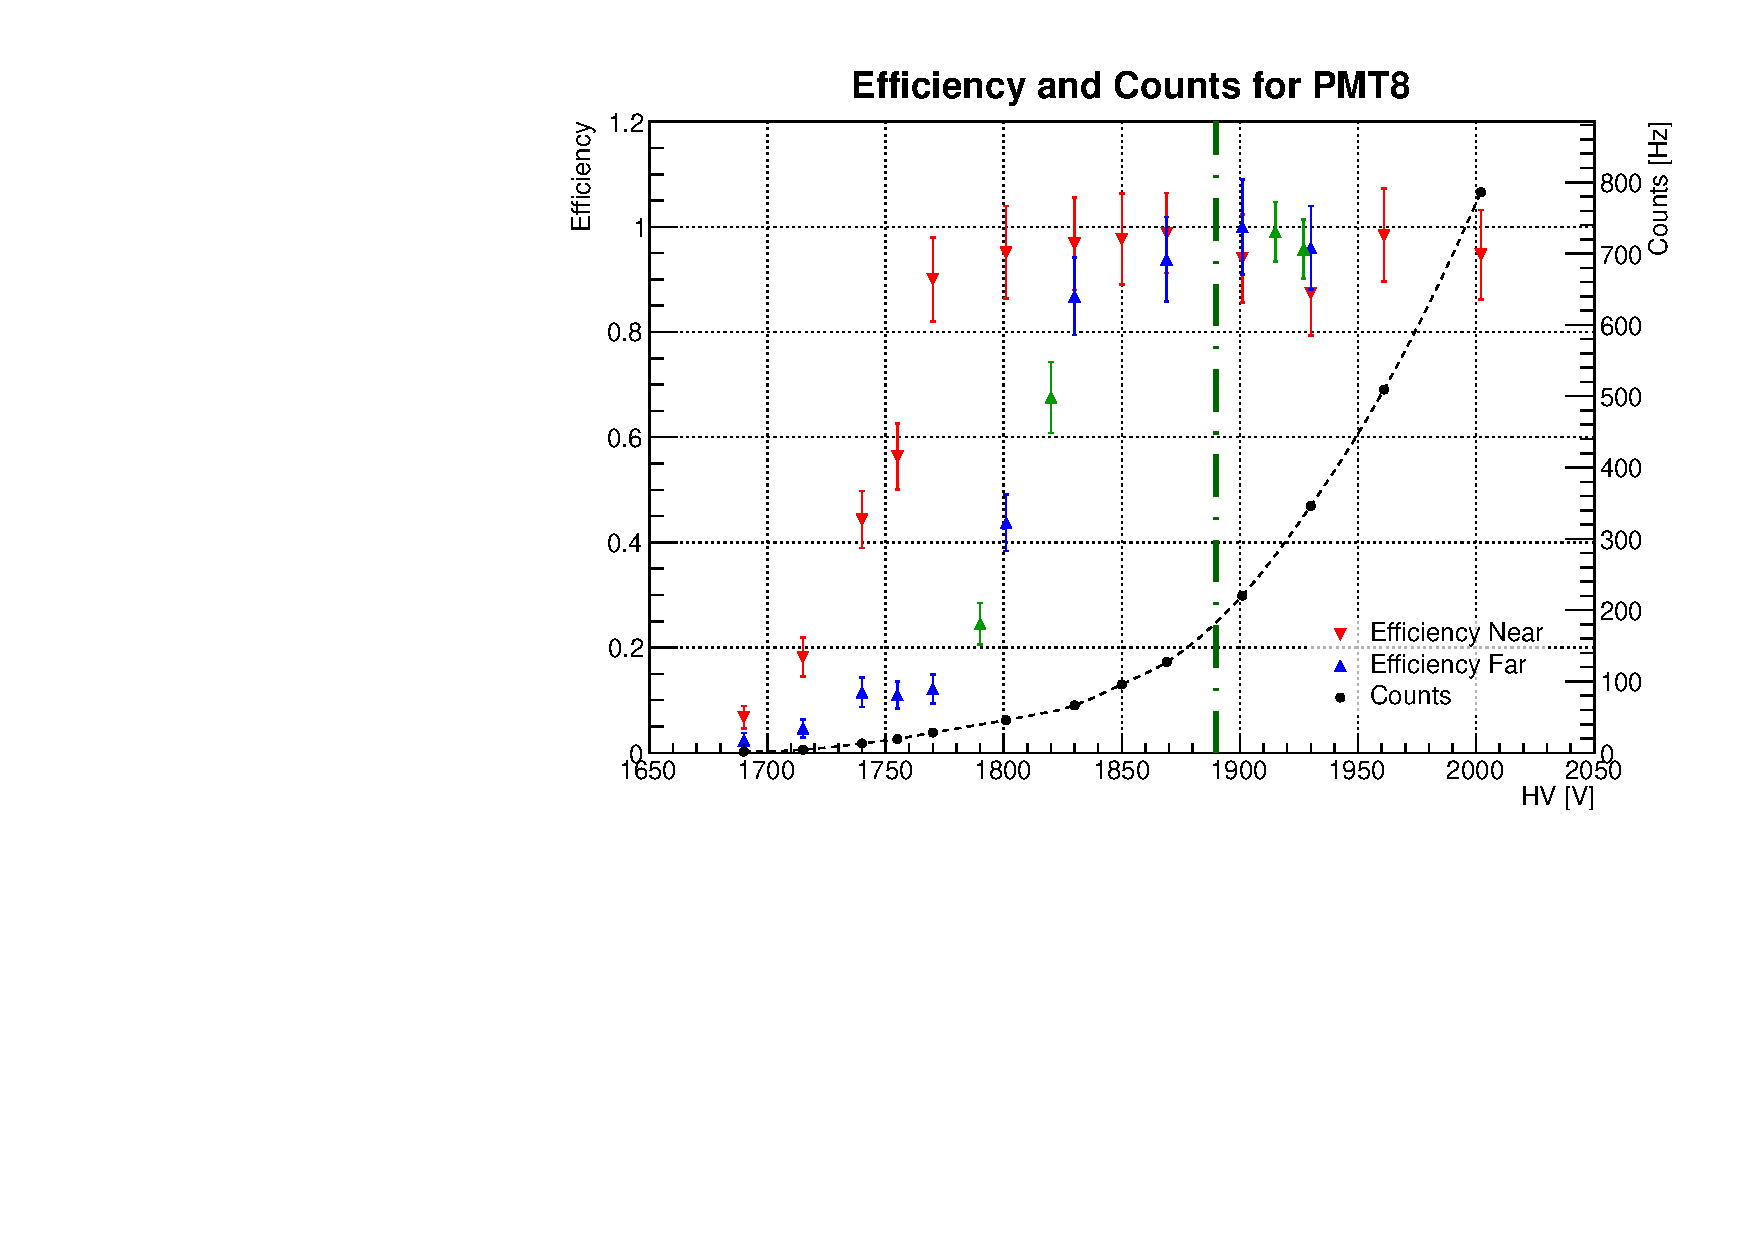
\includegraphics[scale=0.8]{img/eff8.pdf}}
\end{figure}
\begin{figure}[h]
	\centerline{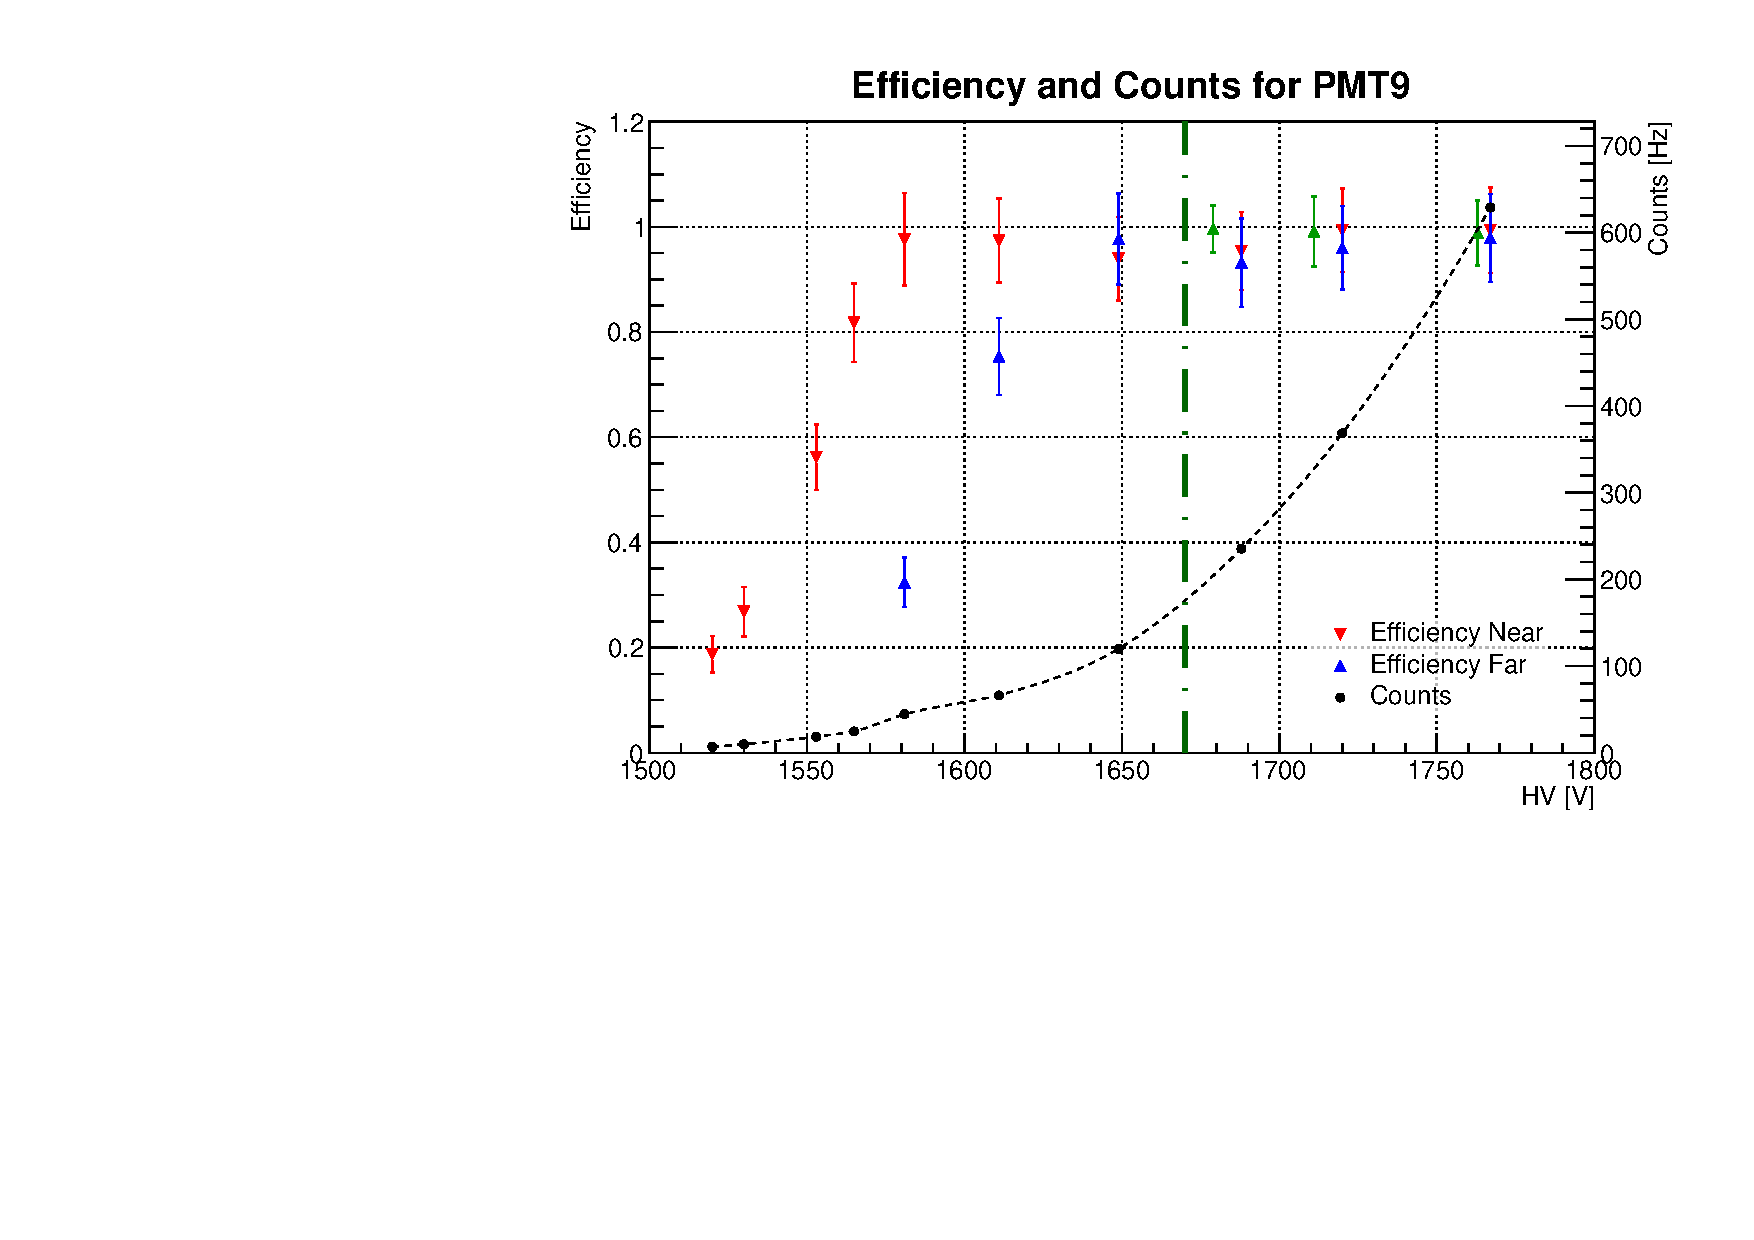
\includegraphics[scale=0.8]{img/eff9.pdf}}
\end{figure}
\begin{figure}[h]
	\centerline{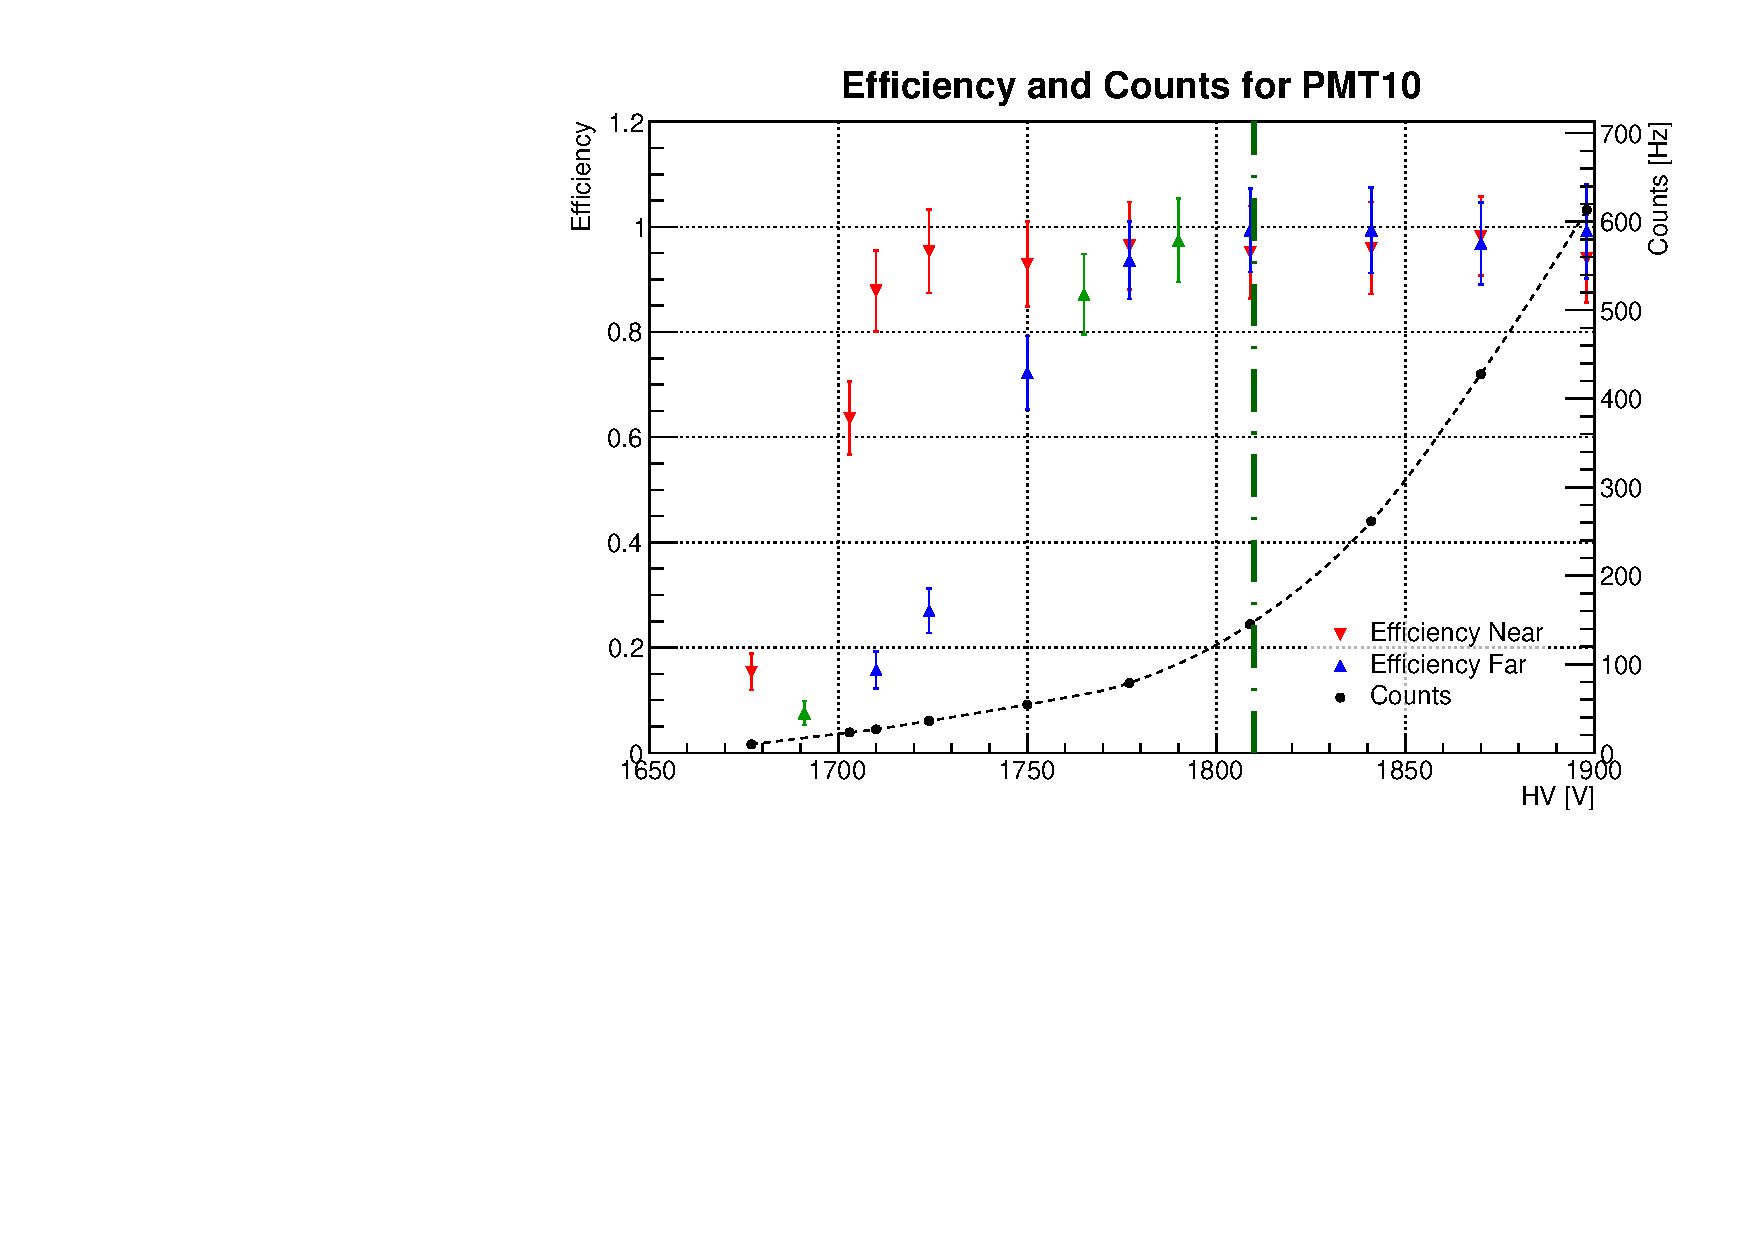
\includegraphics[scale=0.8]{img/eff10.pdf}}
\end{figure}
\begin{figure}[h]
	\centerline{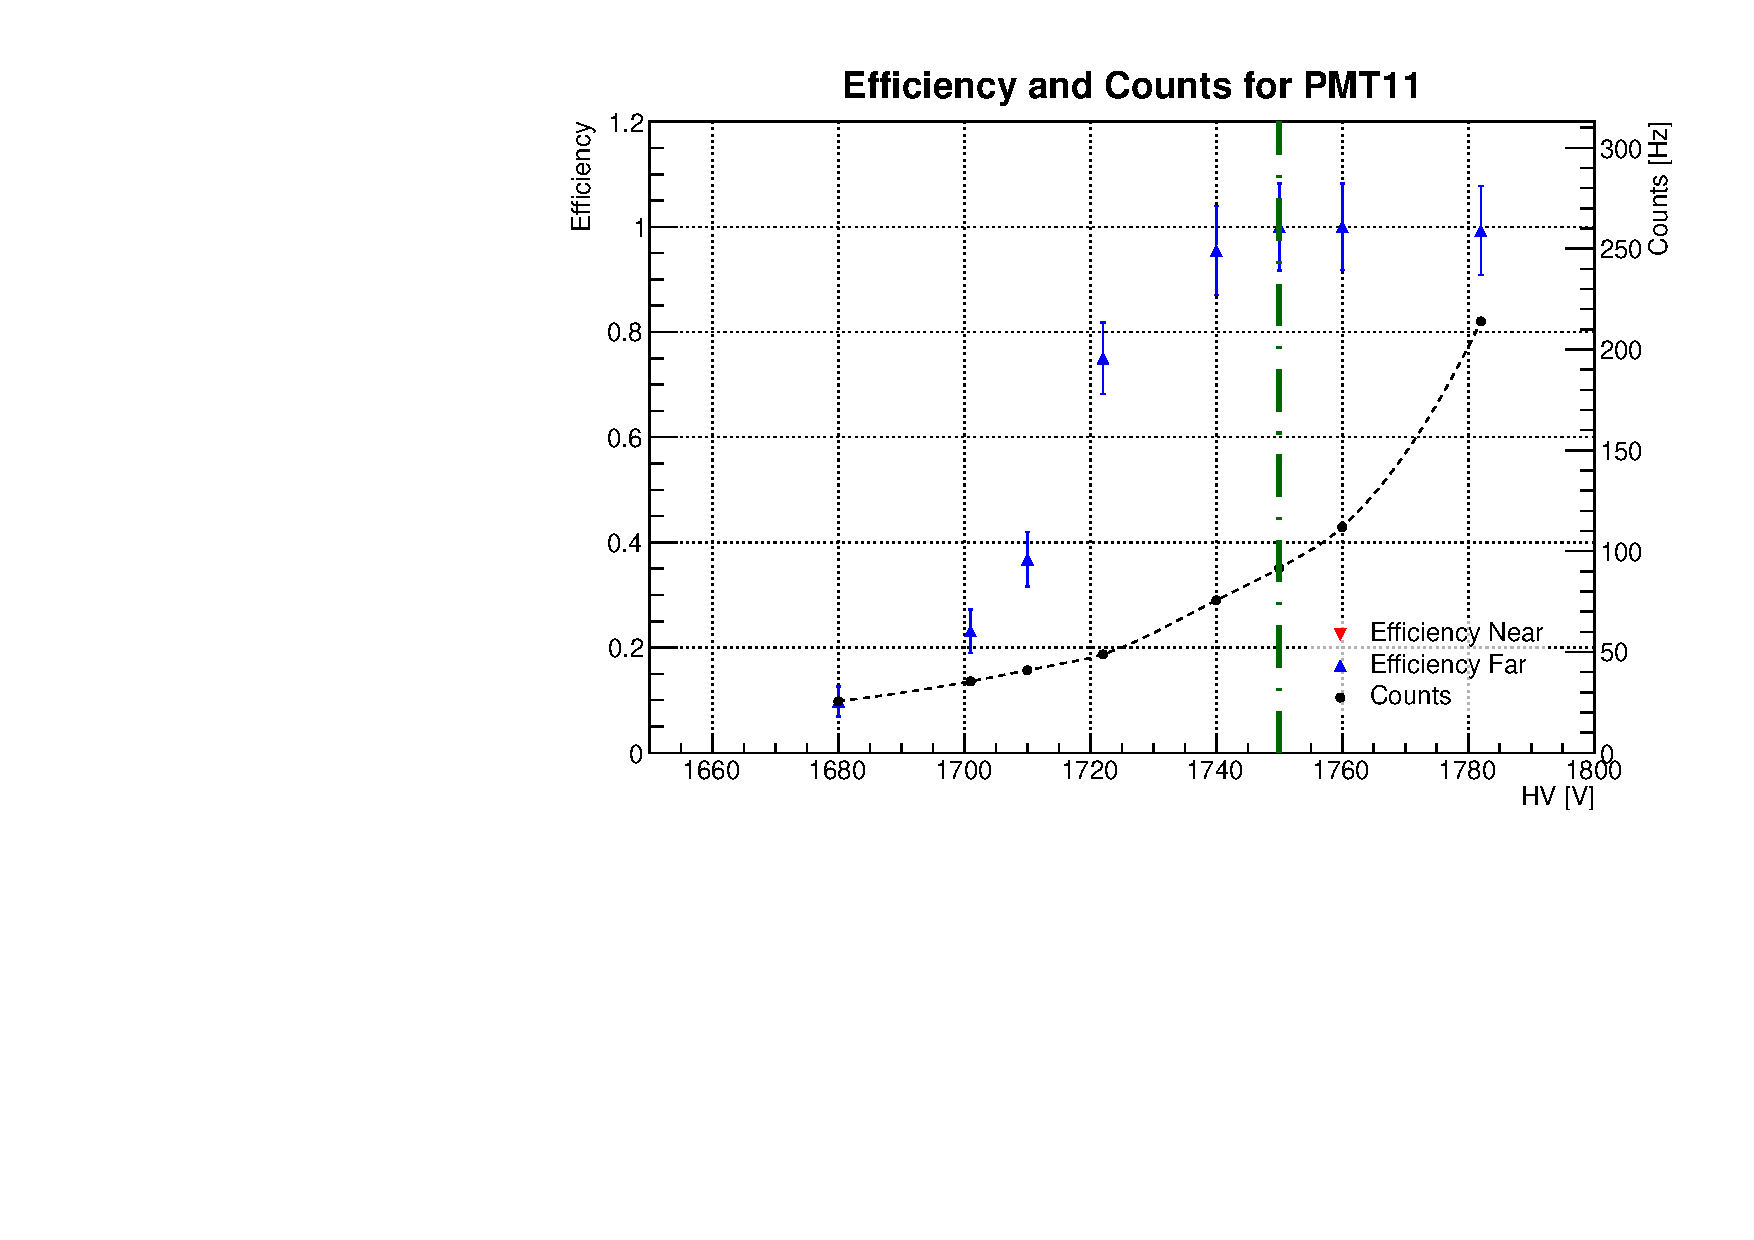
\includegraphics[scale=0.8]{img/eff11.pdf}}
\end{figure}
\begin{figure}[h]
	\centerline{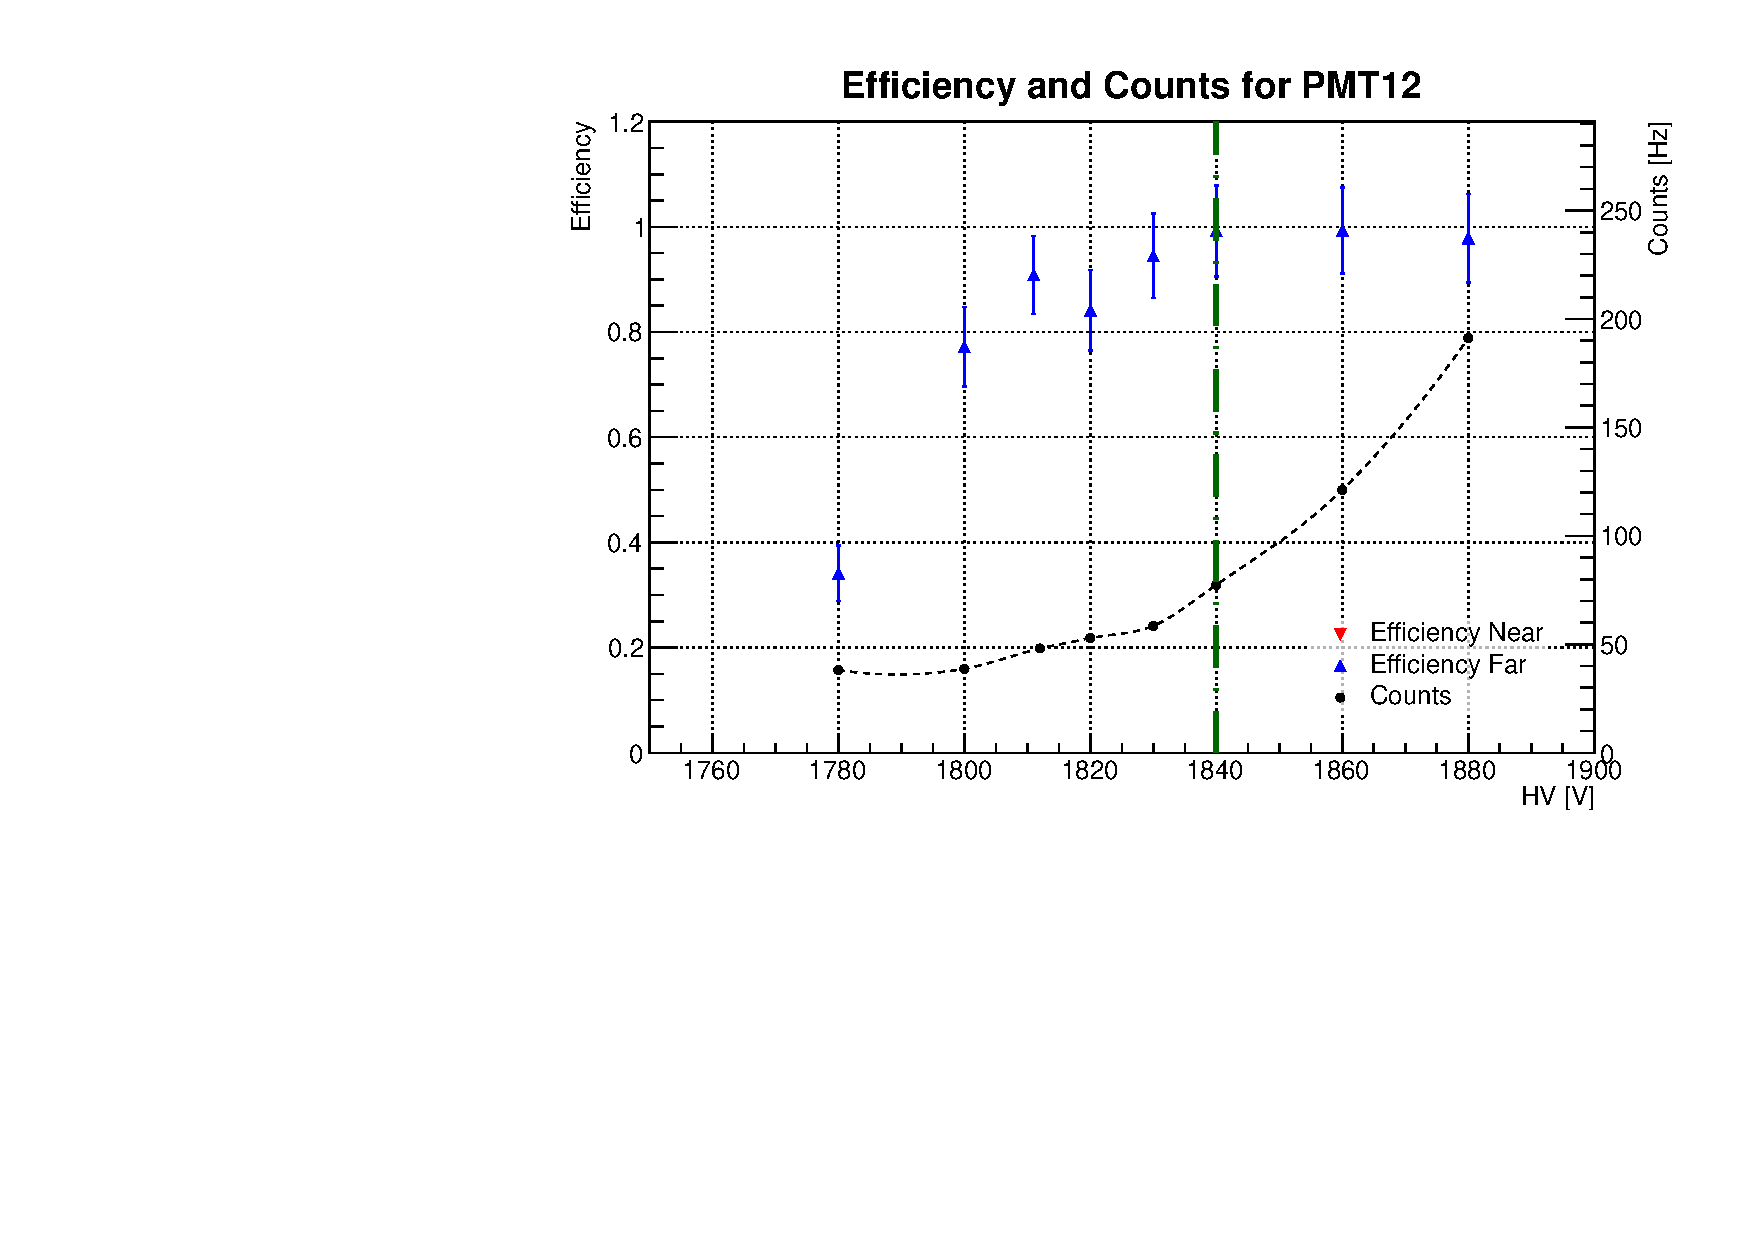
\includegraphics[scale=0.8]{img/eff12.pdf}}
\end{figure}
\begin{figure}[h]
	\centerline{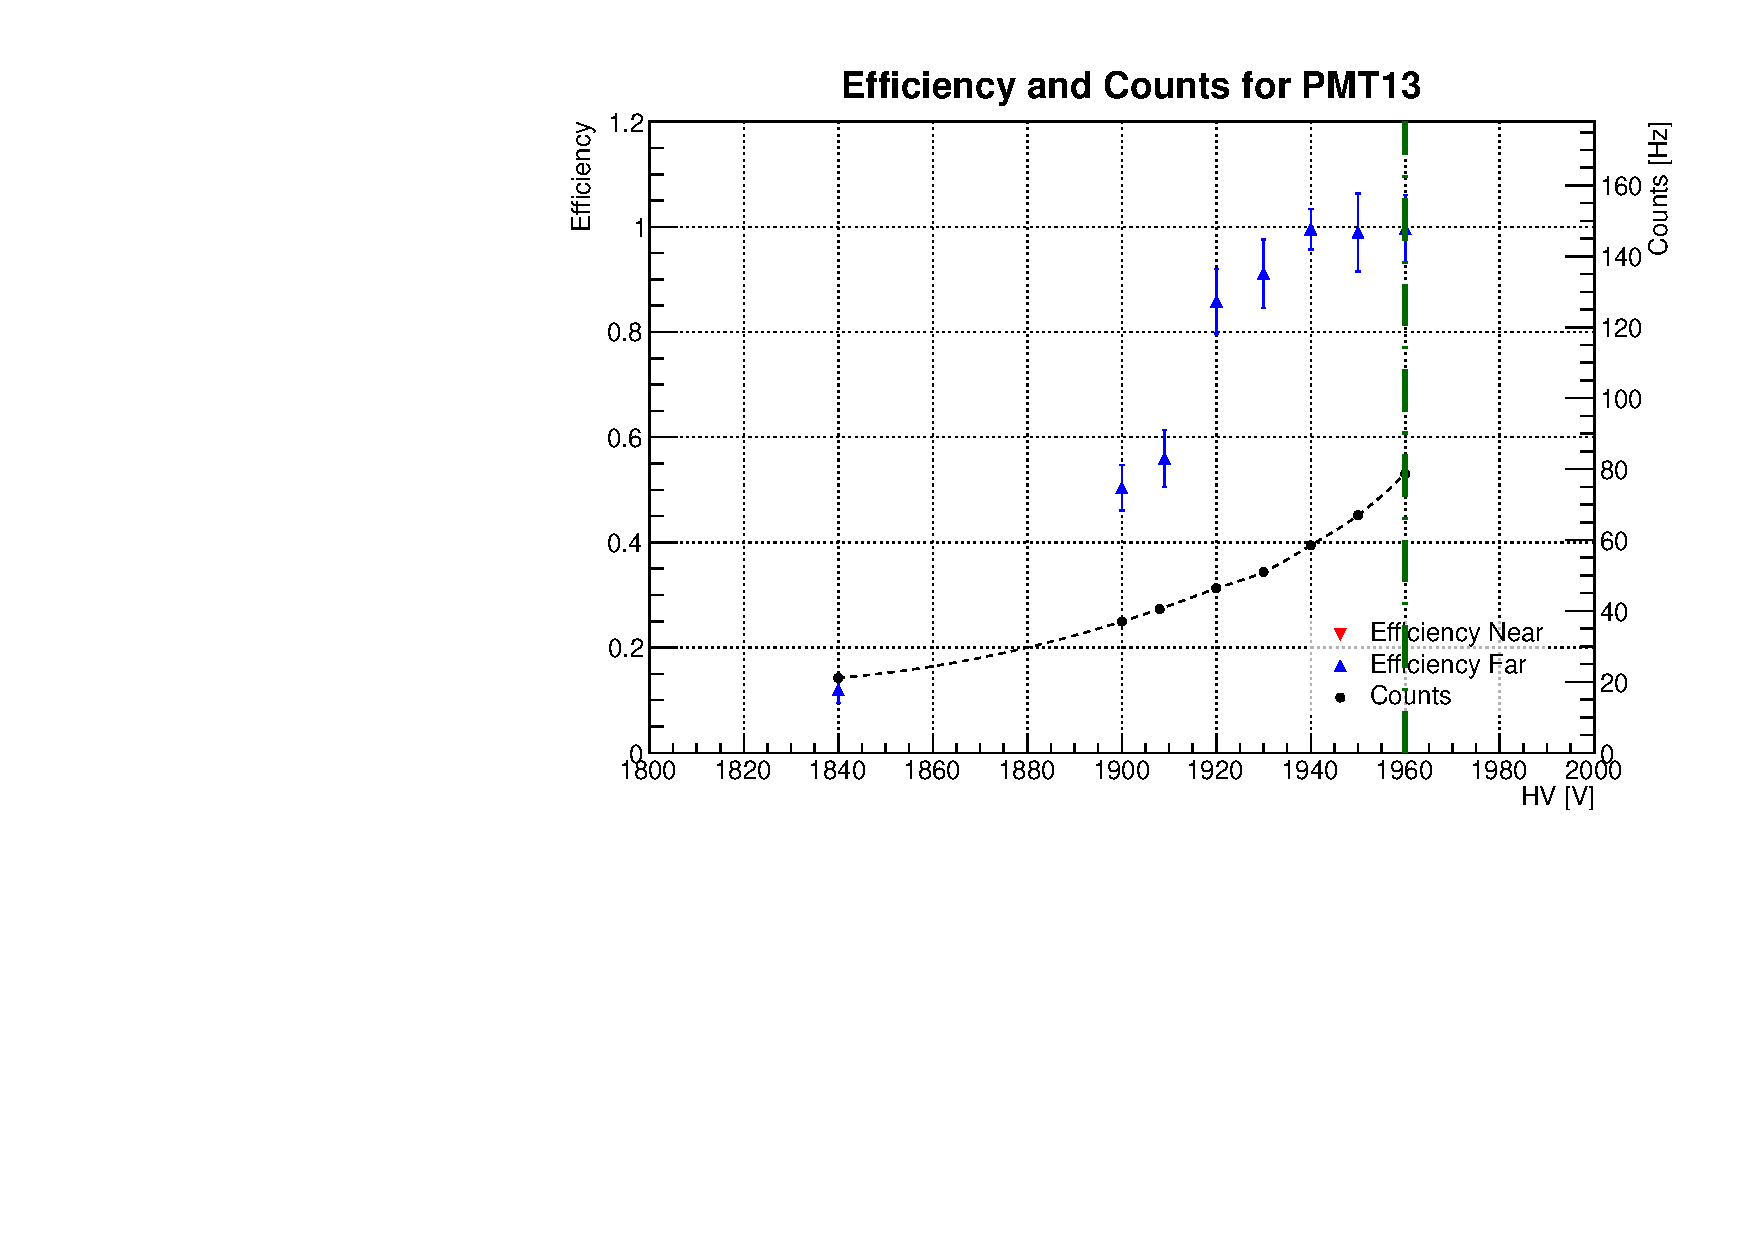
\includegraphics[scale=0.8]{img/eff13.pdf}}
\end{figure}
\begin{figure}[h]
	\centerline{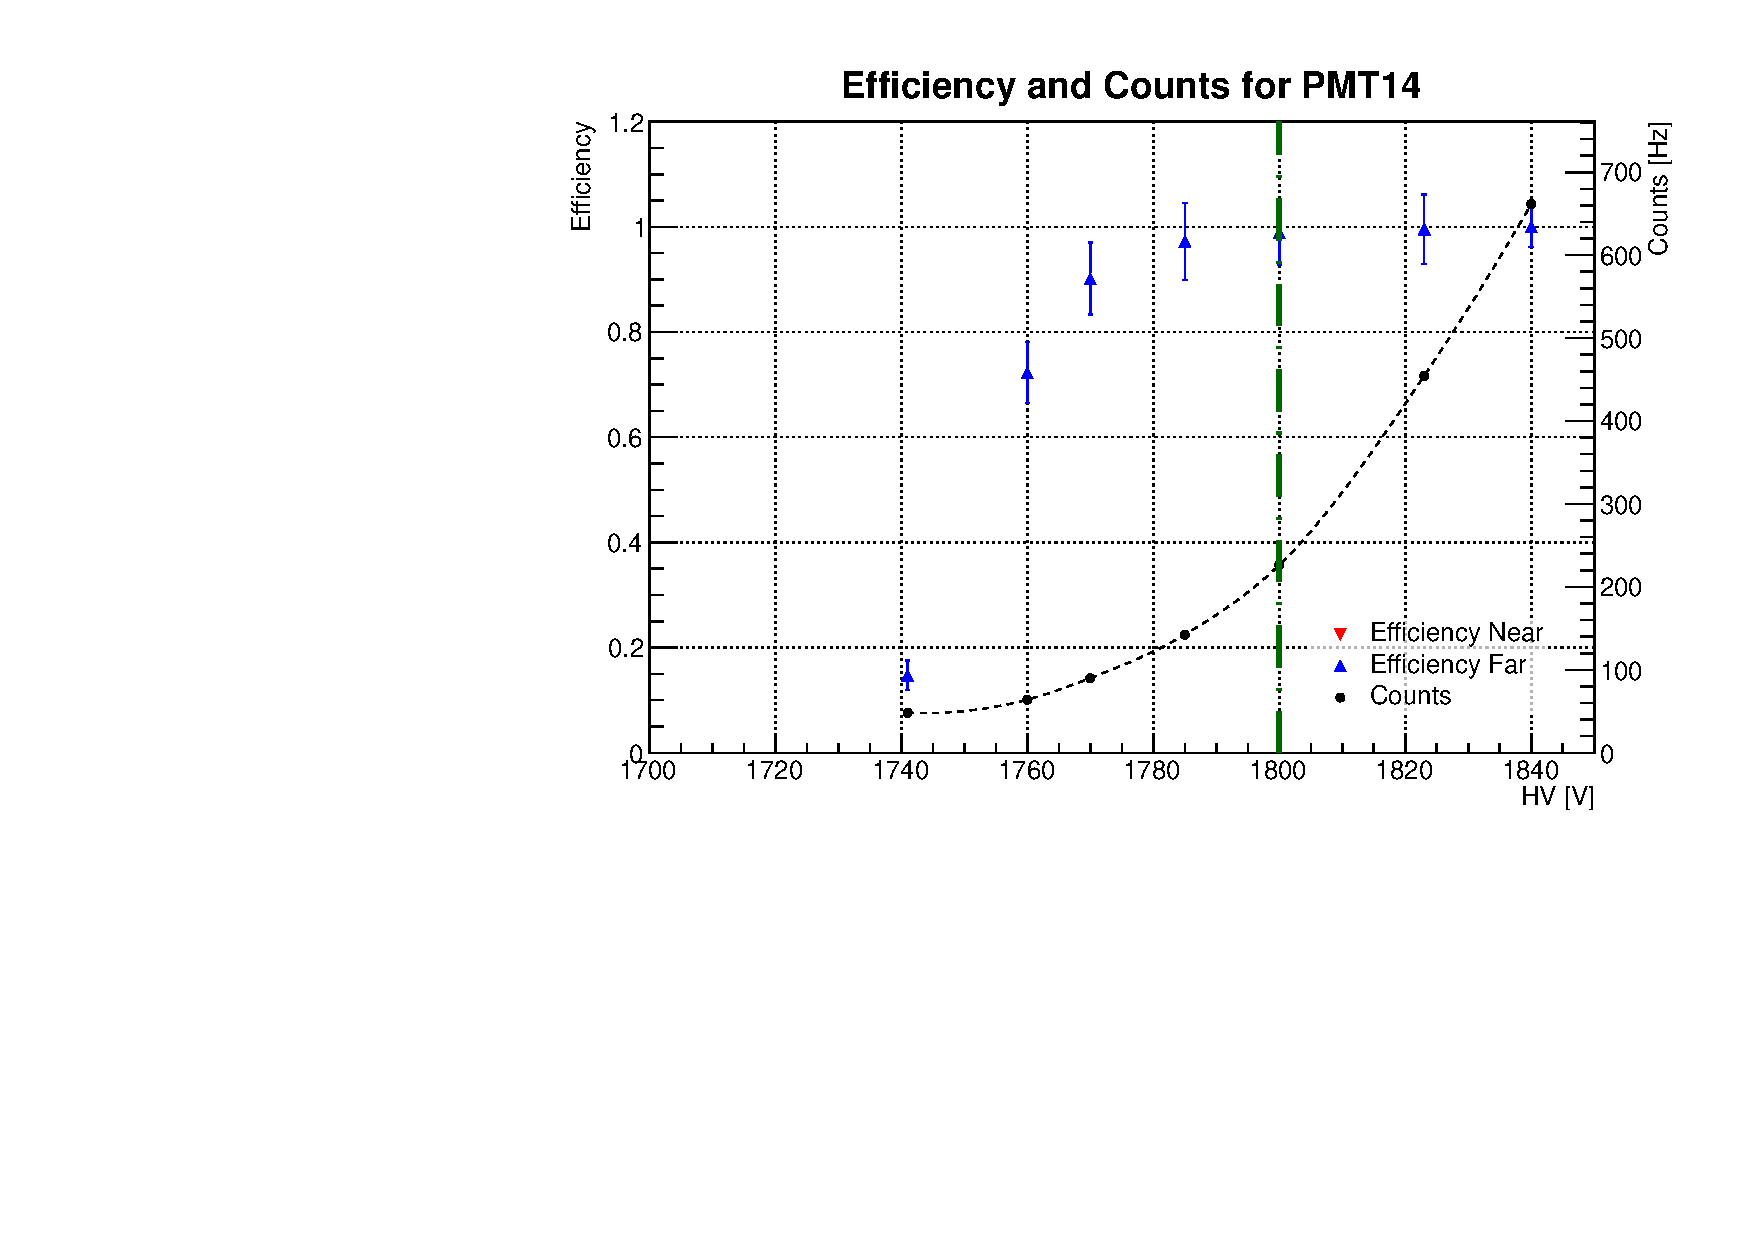
\includegraphics[scale=0.8]{img/eff14.pdf}}
\end{figure}
%\begin{figure}[h]
%	\centerline{
%		\subfloat
%		{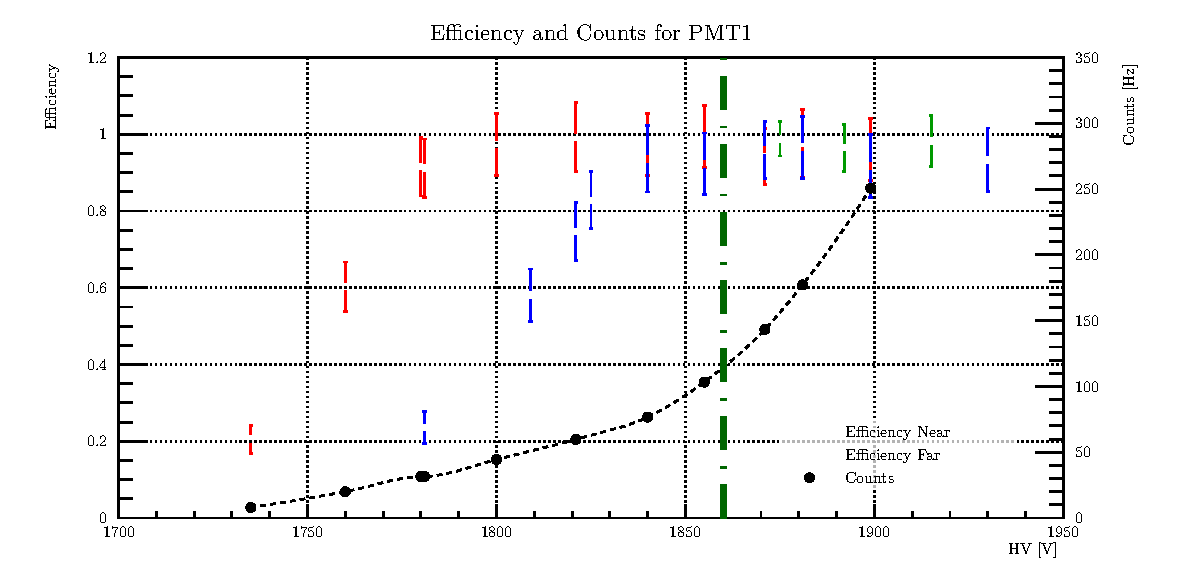
\includegraphics[scale=0.5]{img/eff1.pdf}}
%		\subfloat
%		{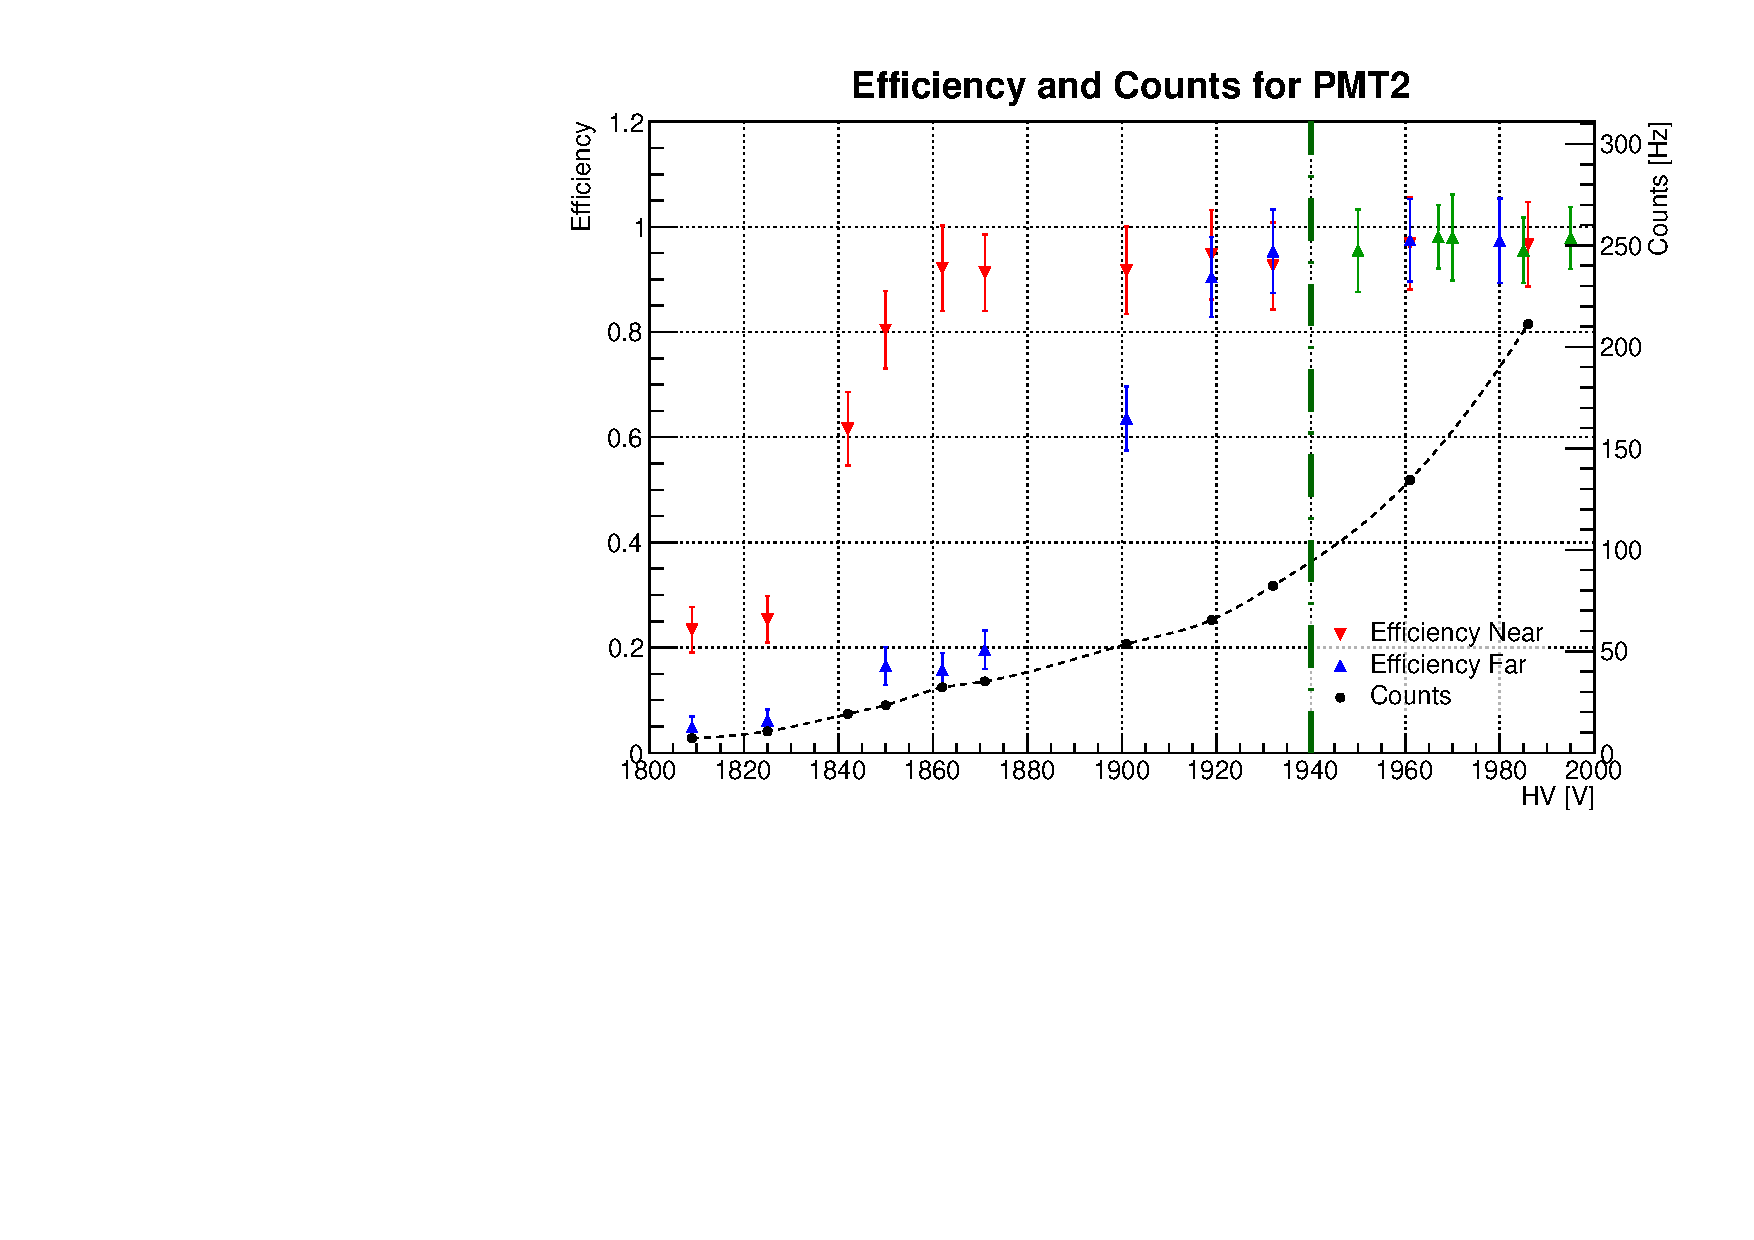
\includegraphics[scale=0.5]{img/eff2.pdf}}}
%	\centerline{
%		\subfloat
%		{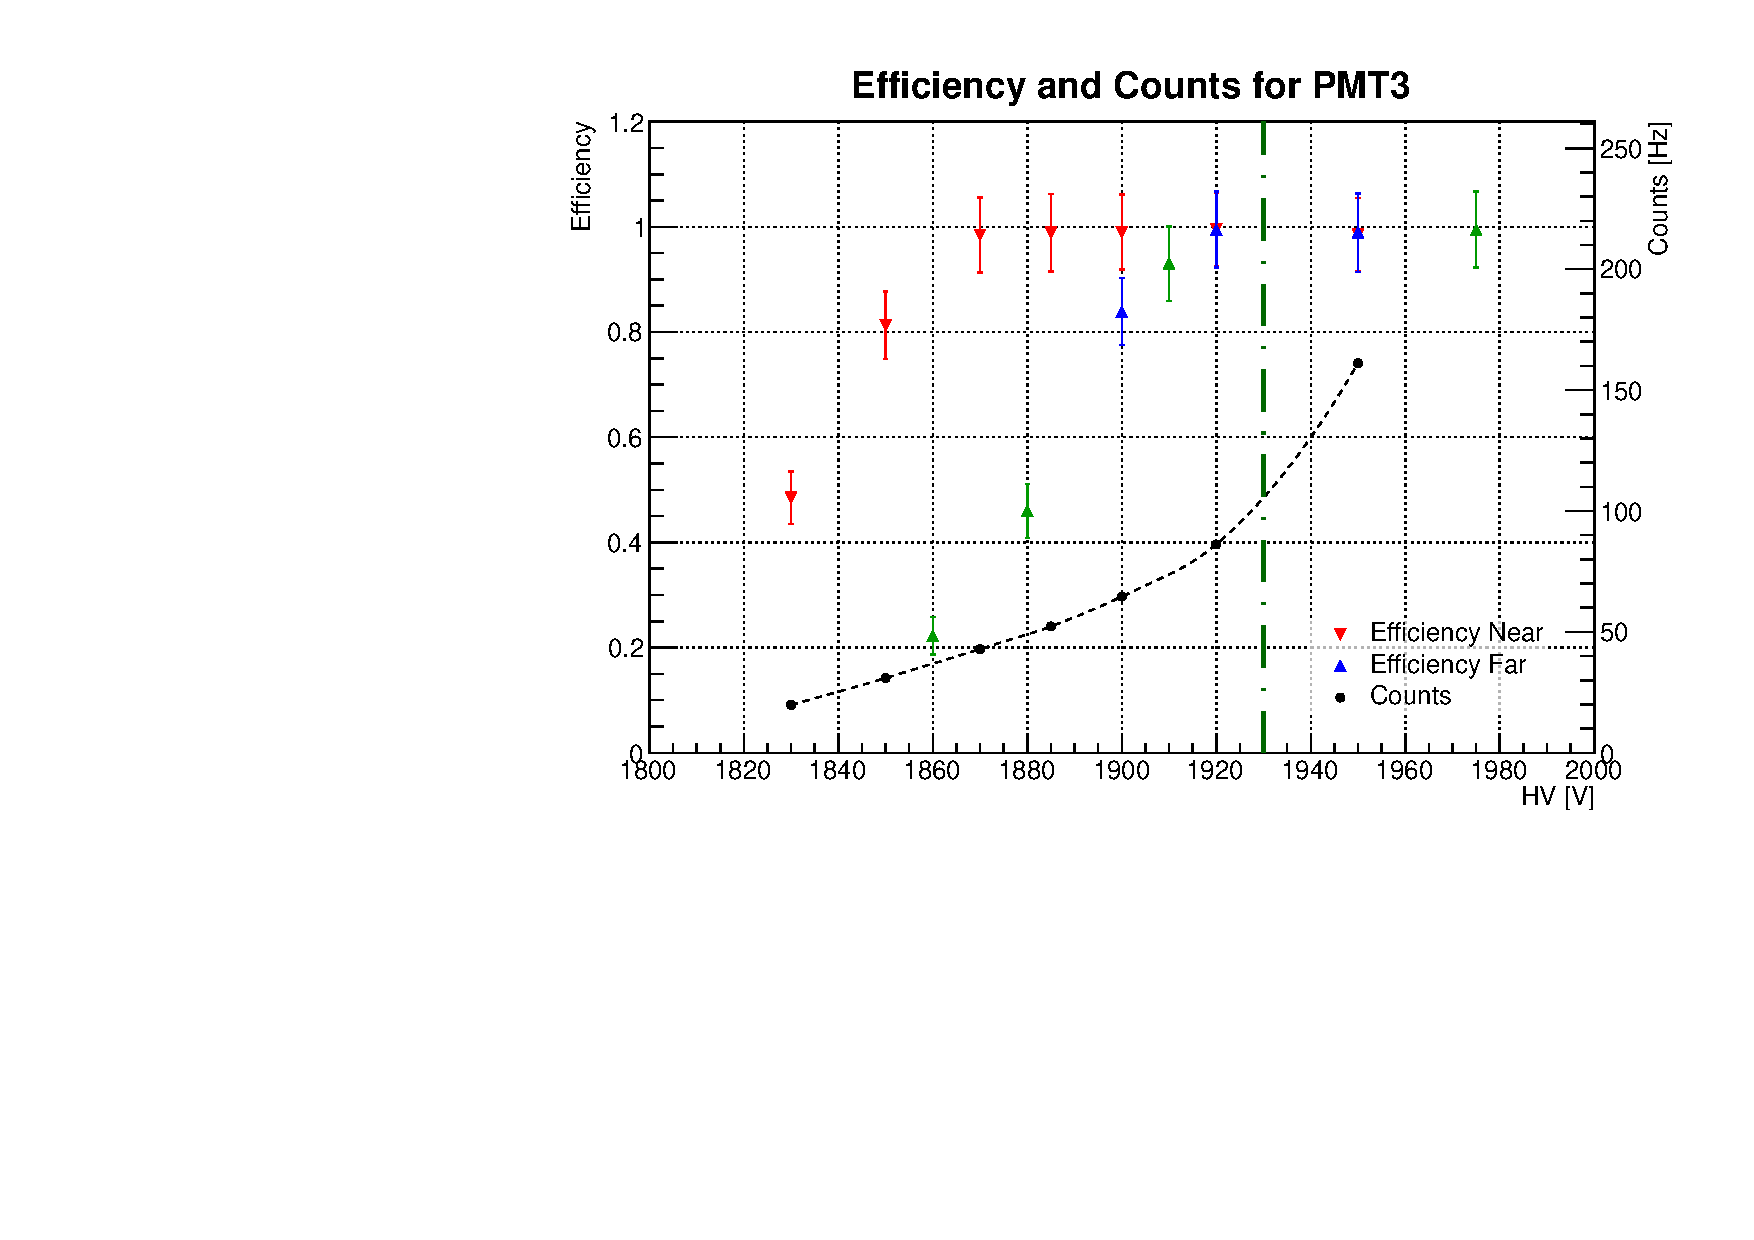
\includegraphics[scale=0.5]{img/eff3.pdf}}
%		\subfloat
%		{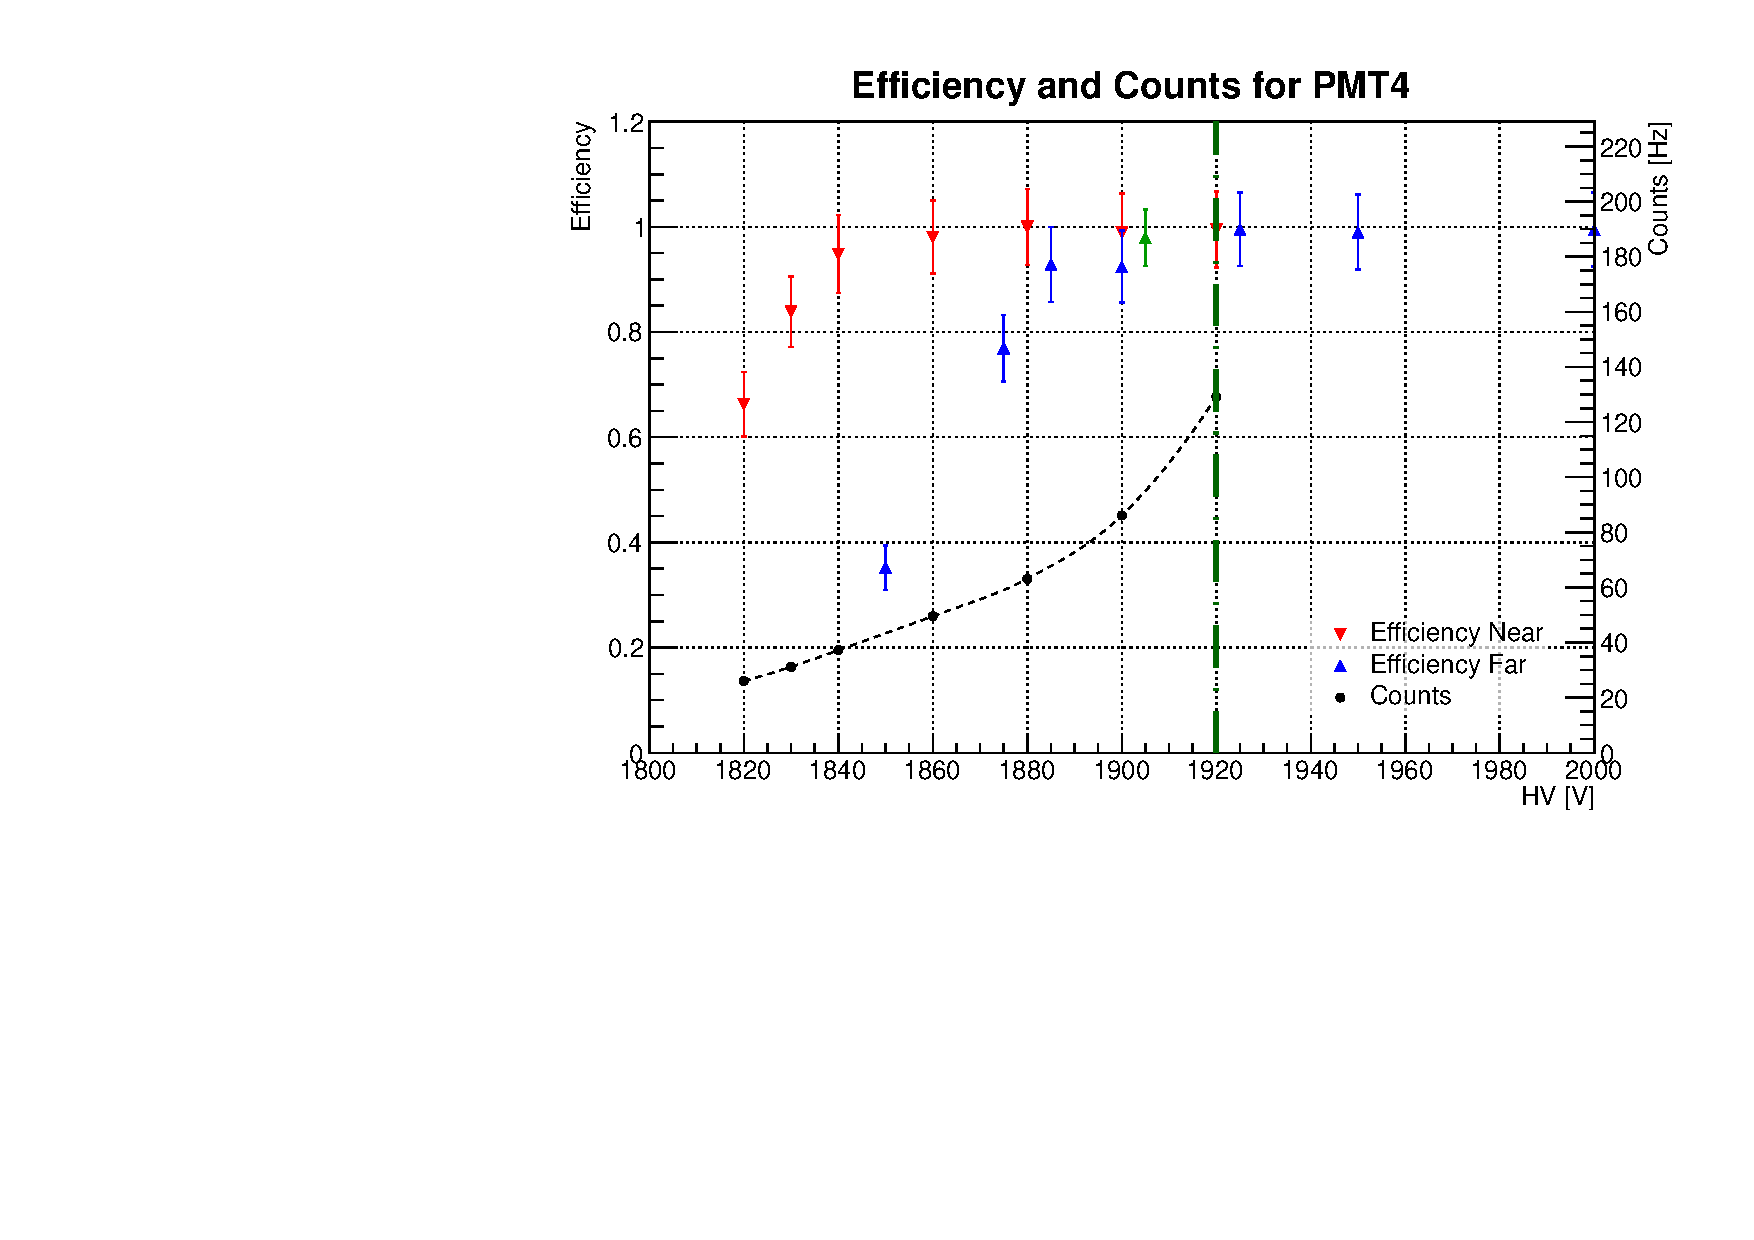
\includegraphics[scale=0.5]{img/eff4.pdf}}}
%\end{figure}
%\begin{figure}[h]
%	\centerline{
%		\subfloat
%		{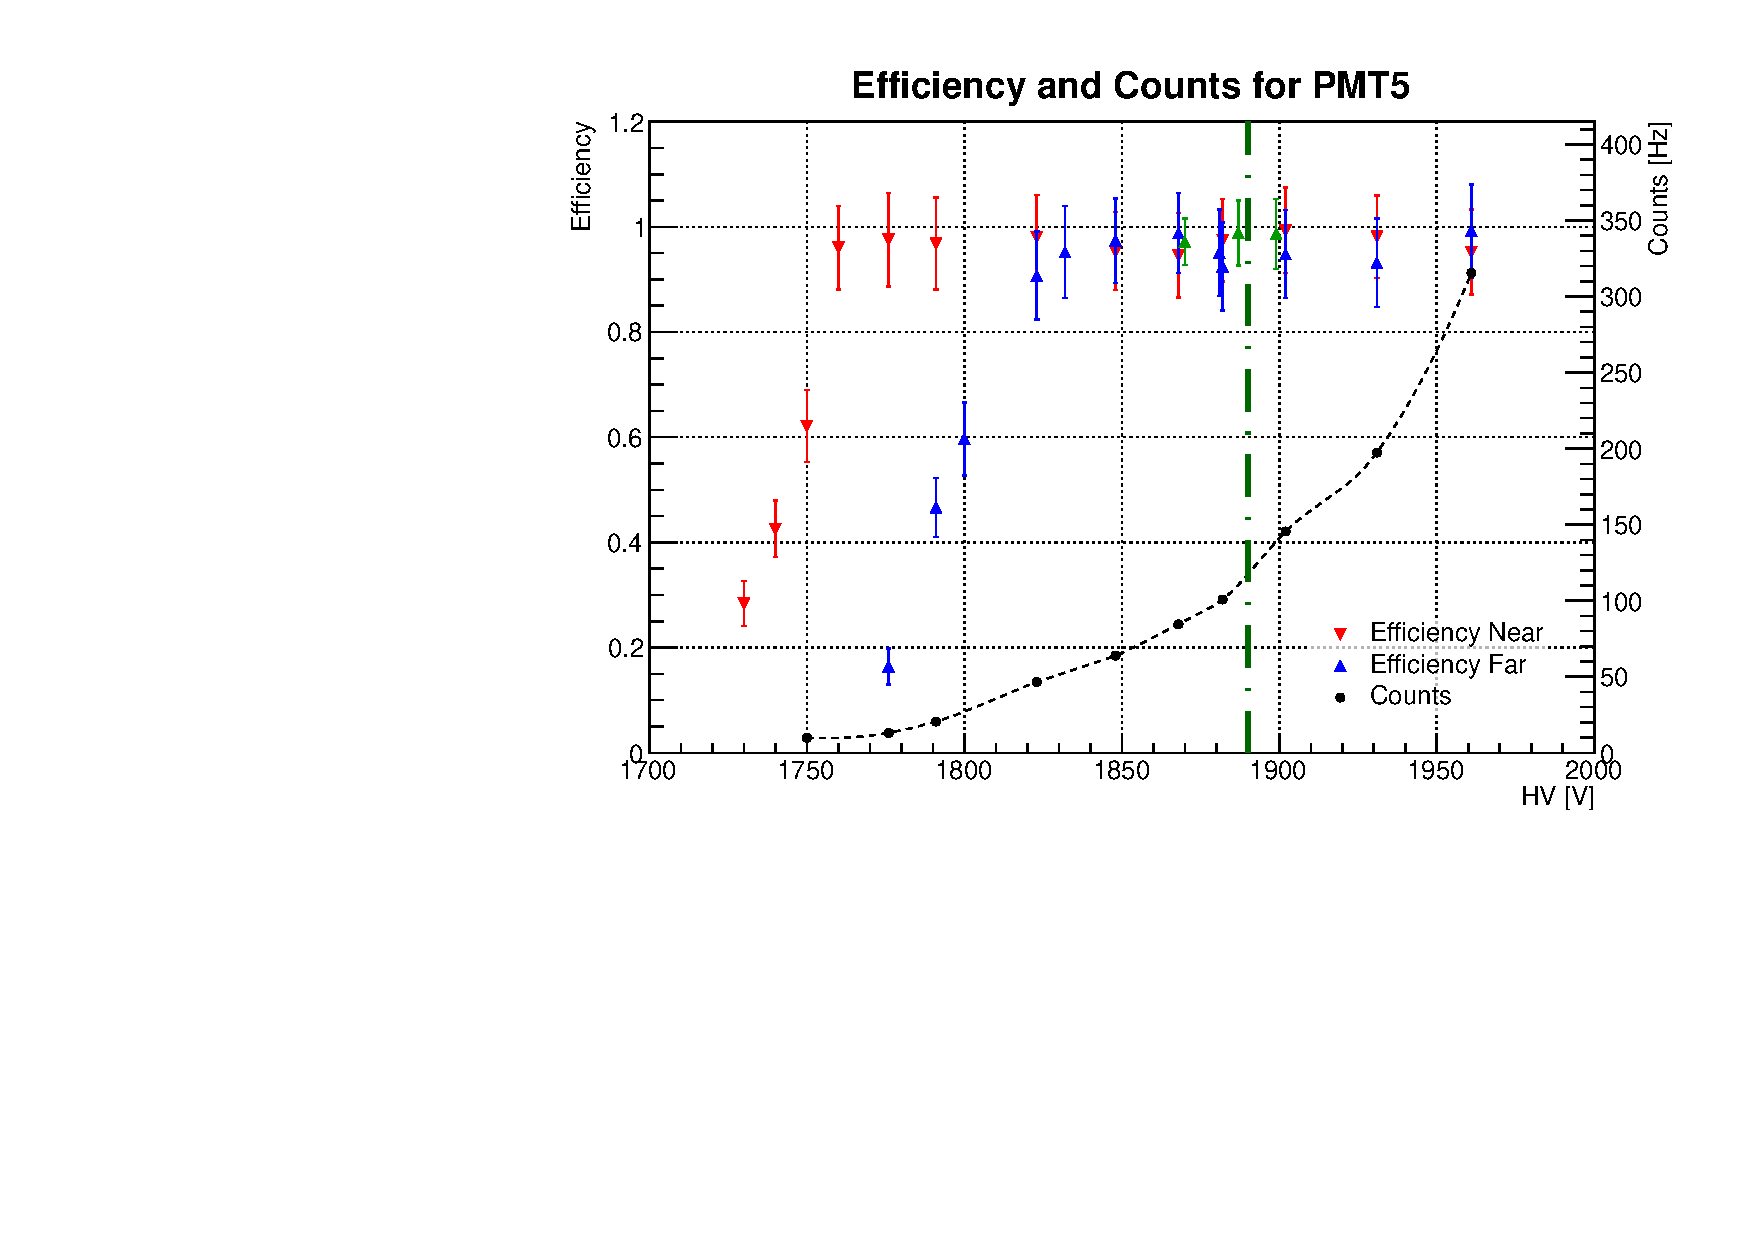
\includegraphics[scale=0.5]{img/eff5.pdf}}
%		\subfloat
%		{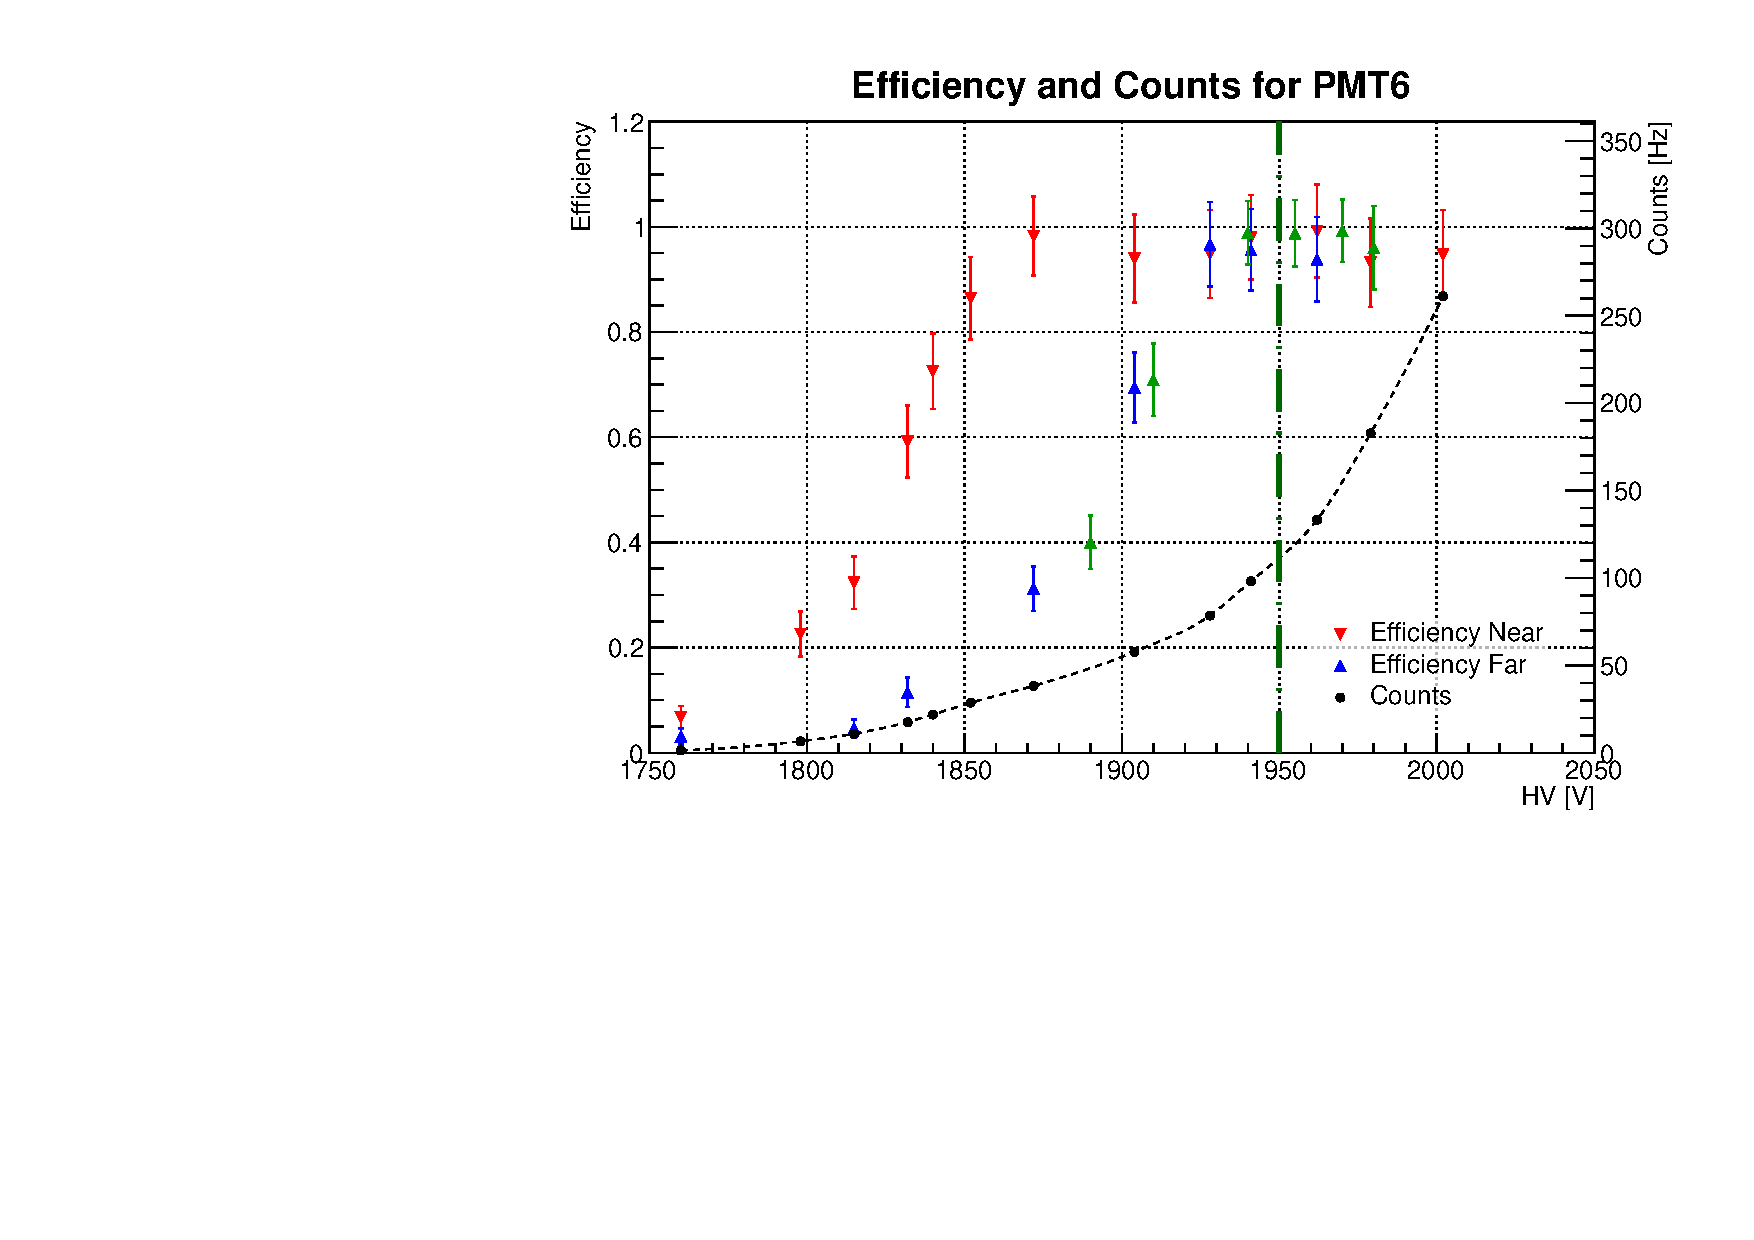
\includegraphics[scale=0.5]{img/eff6.pdf}}}
%	\centerline{
%		\subfloat
%		{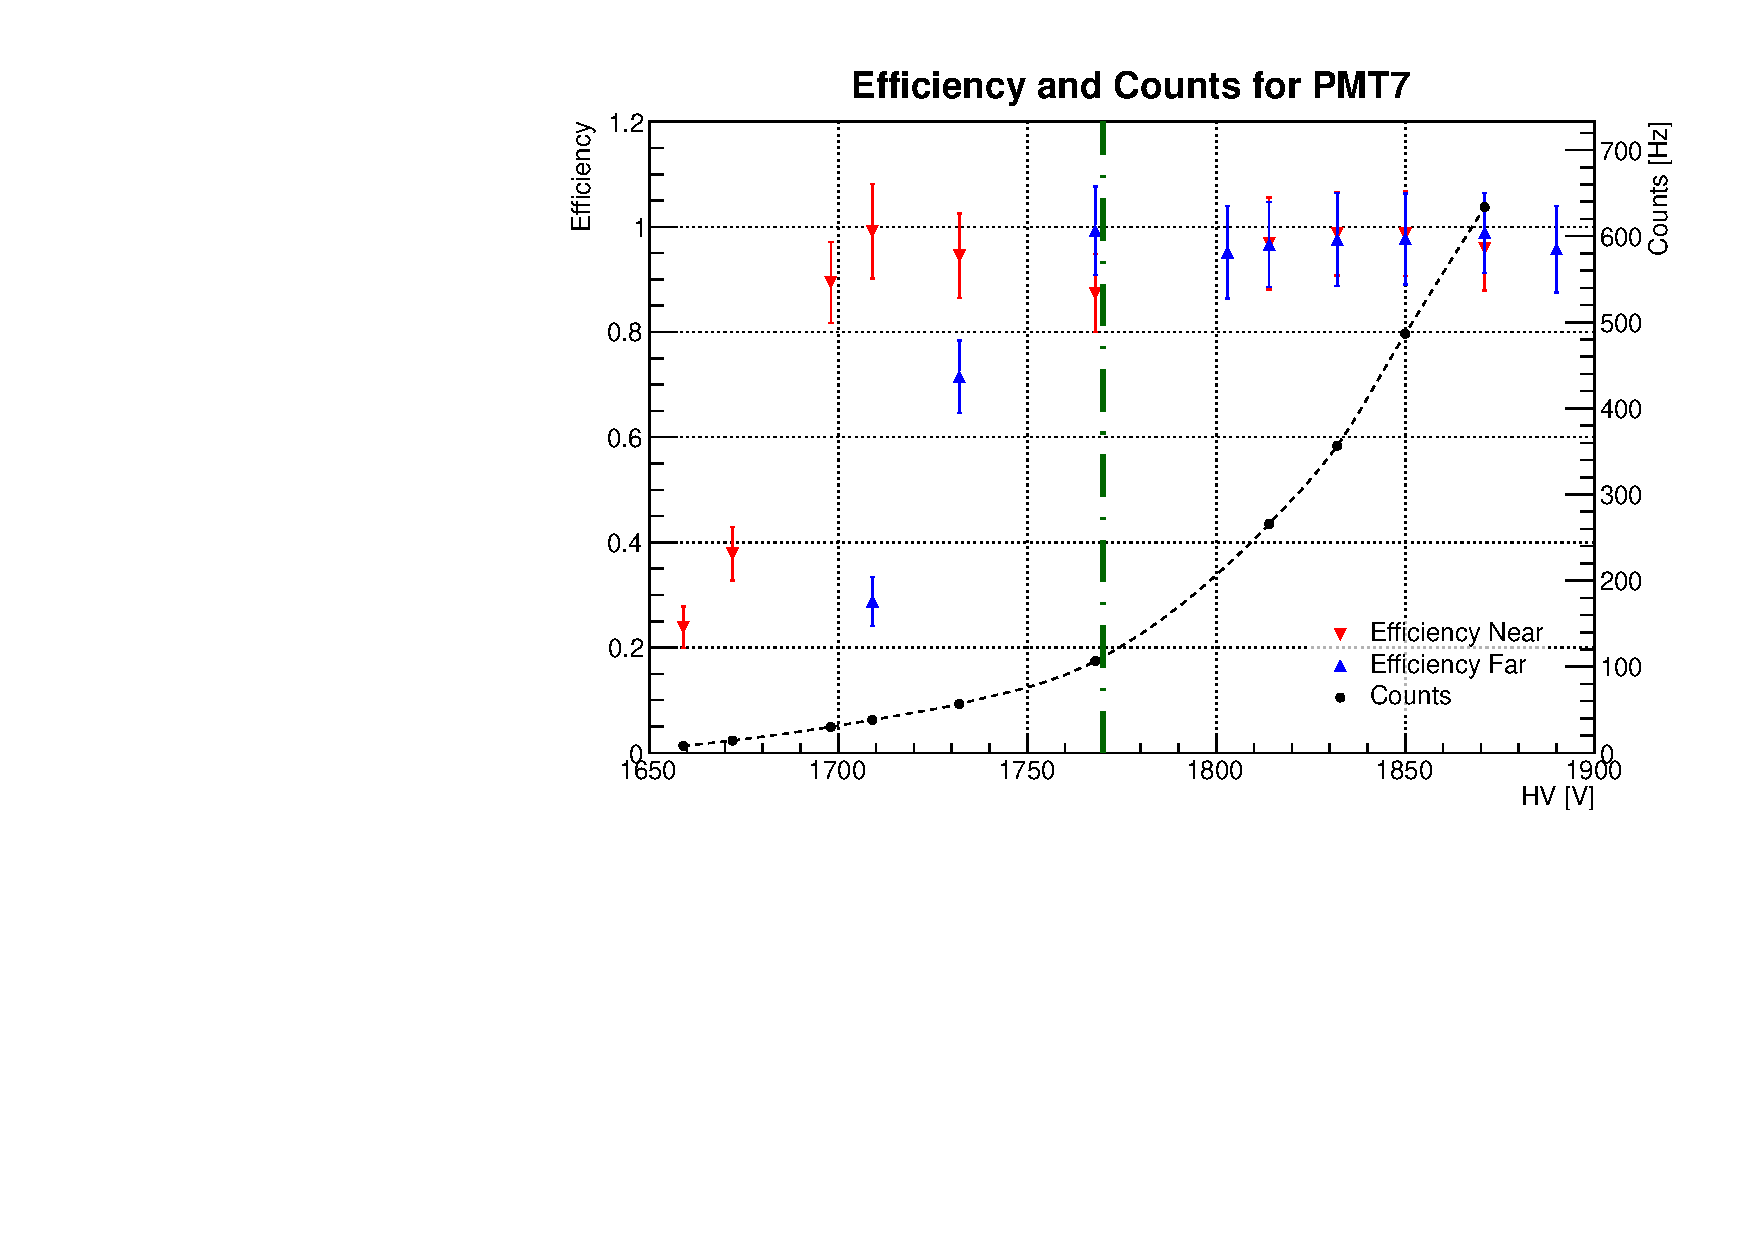
\includegraphics[scale=0.5]{img/eff7.pdf}}
%		\subfloat
%		{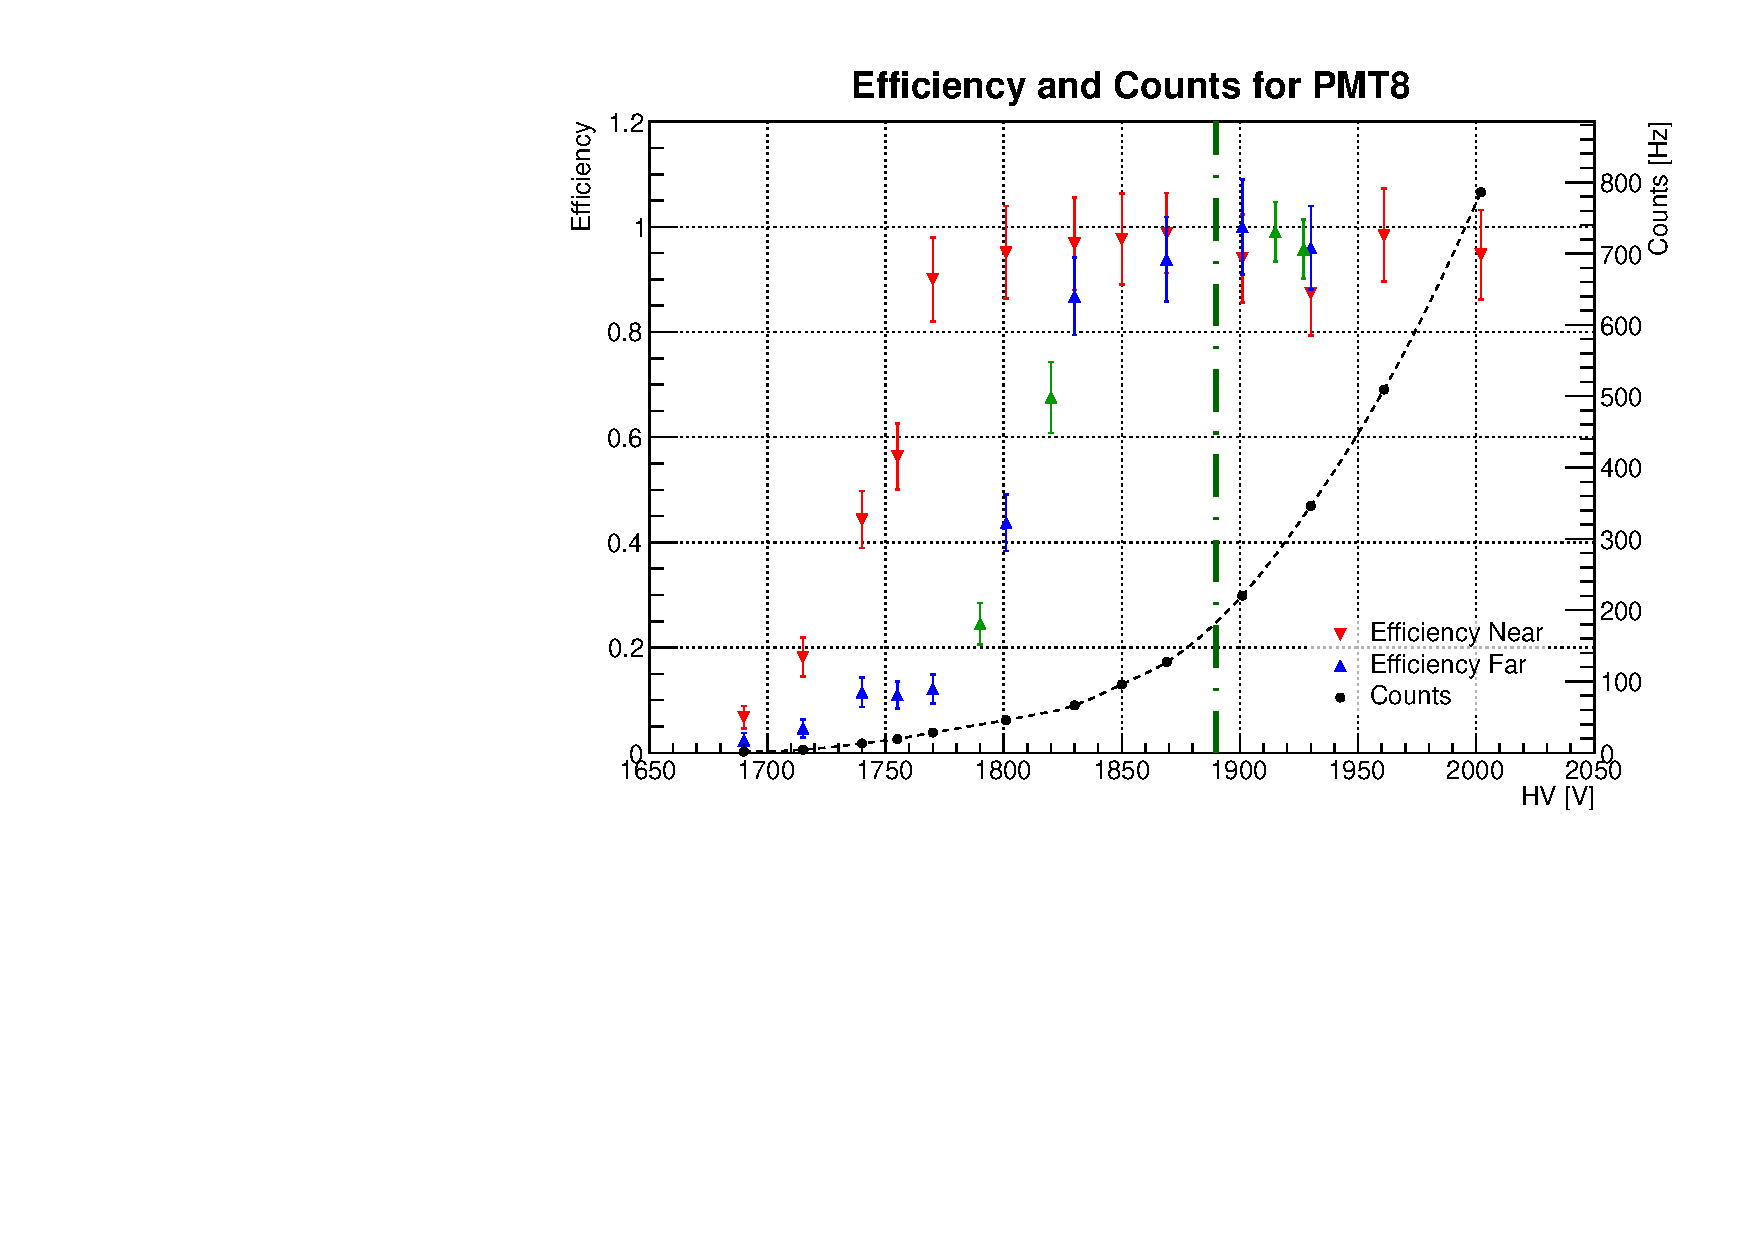
\includegraphics[scale=0.5]{img/eff8.pdf}}}
%\end{figure}
%\begin{figure}[h]
%	\centerline{
%		\subfloat
%		{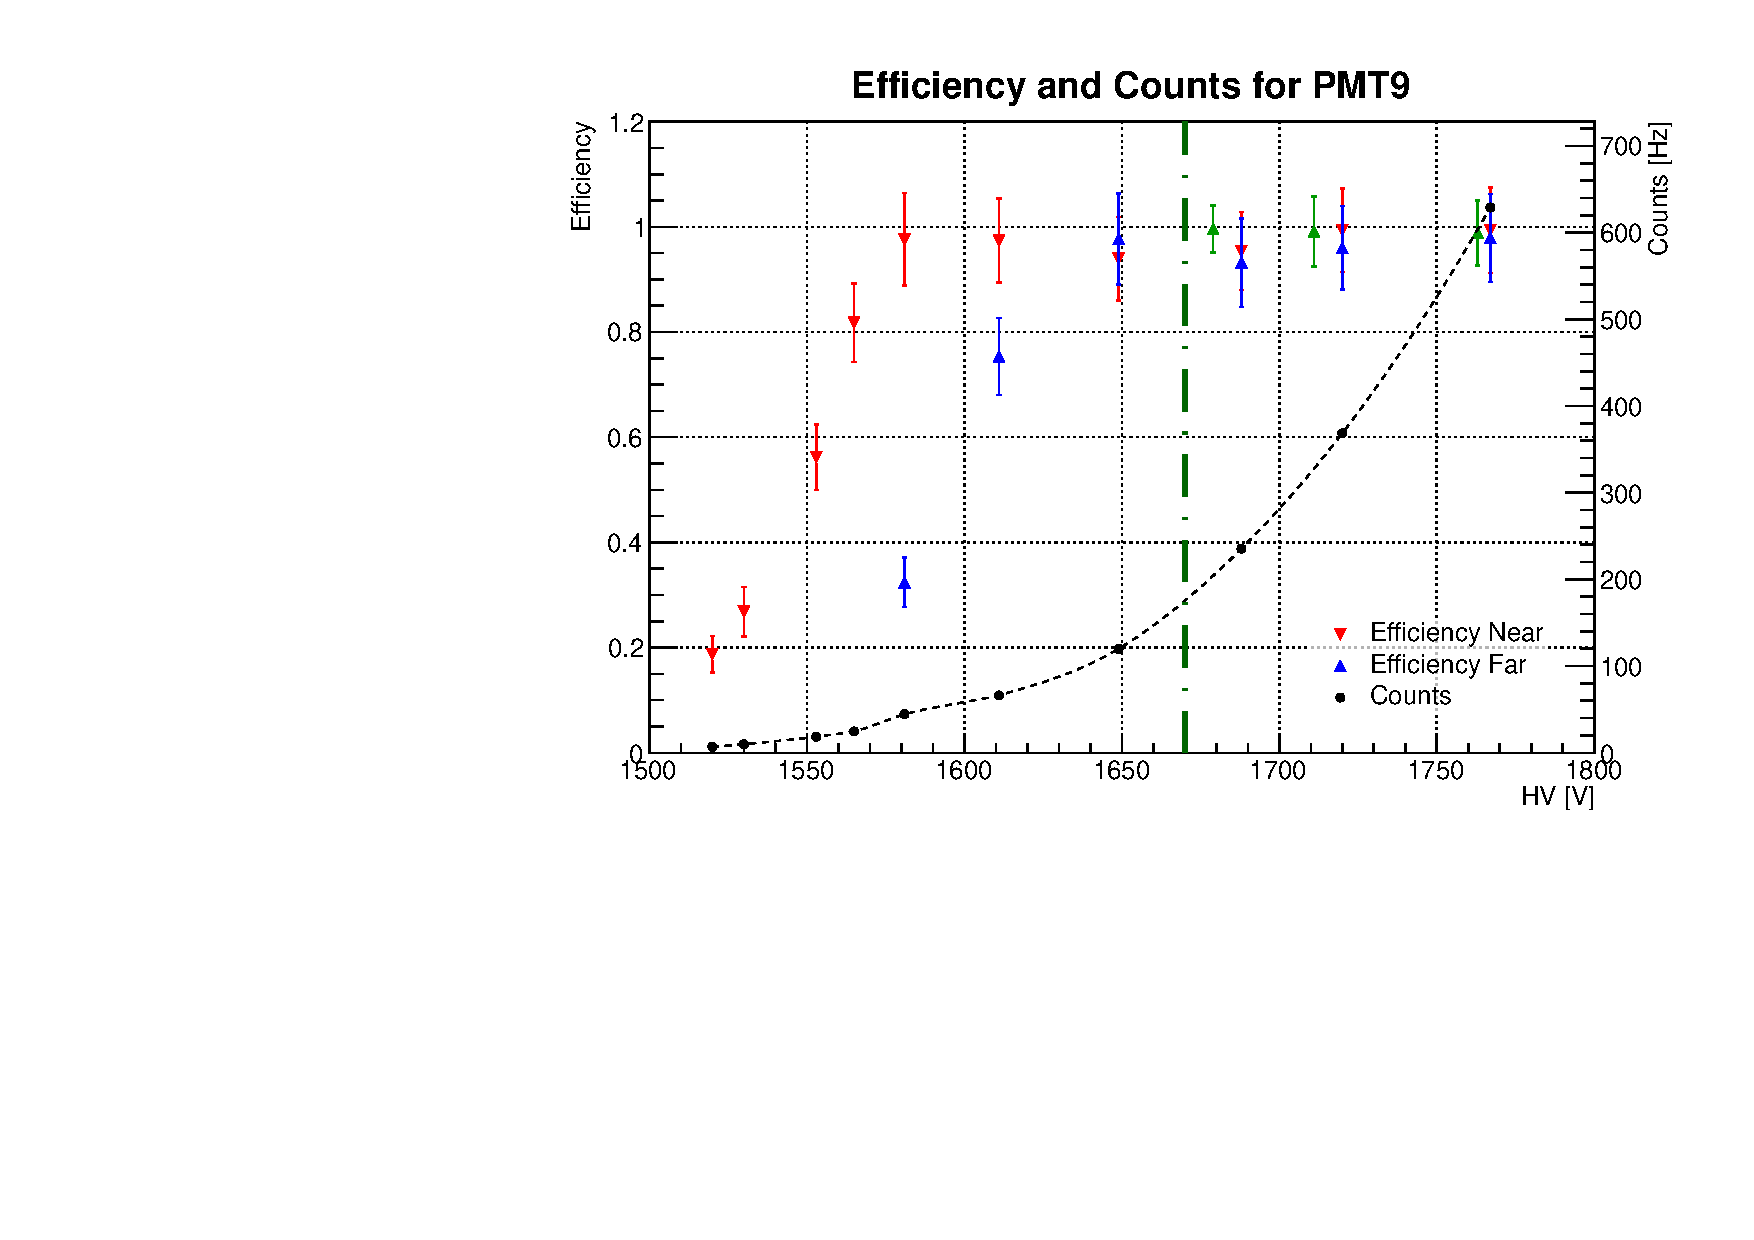
\includegraphics[scale=0.5]{img/eff9.pdf}}
%		\subfloat
%		{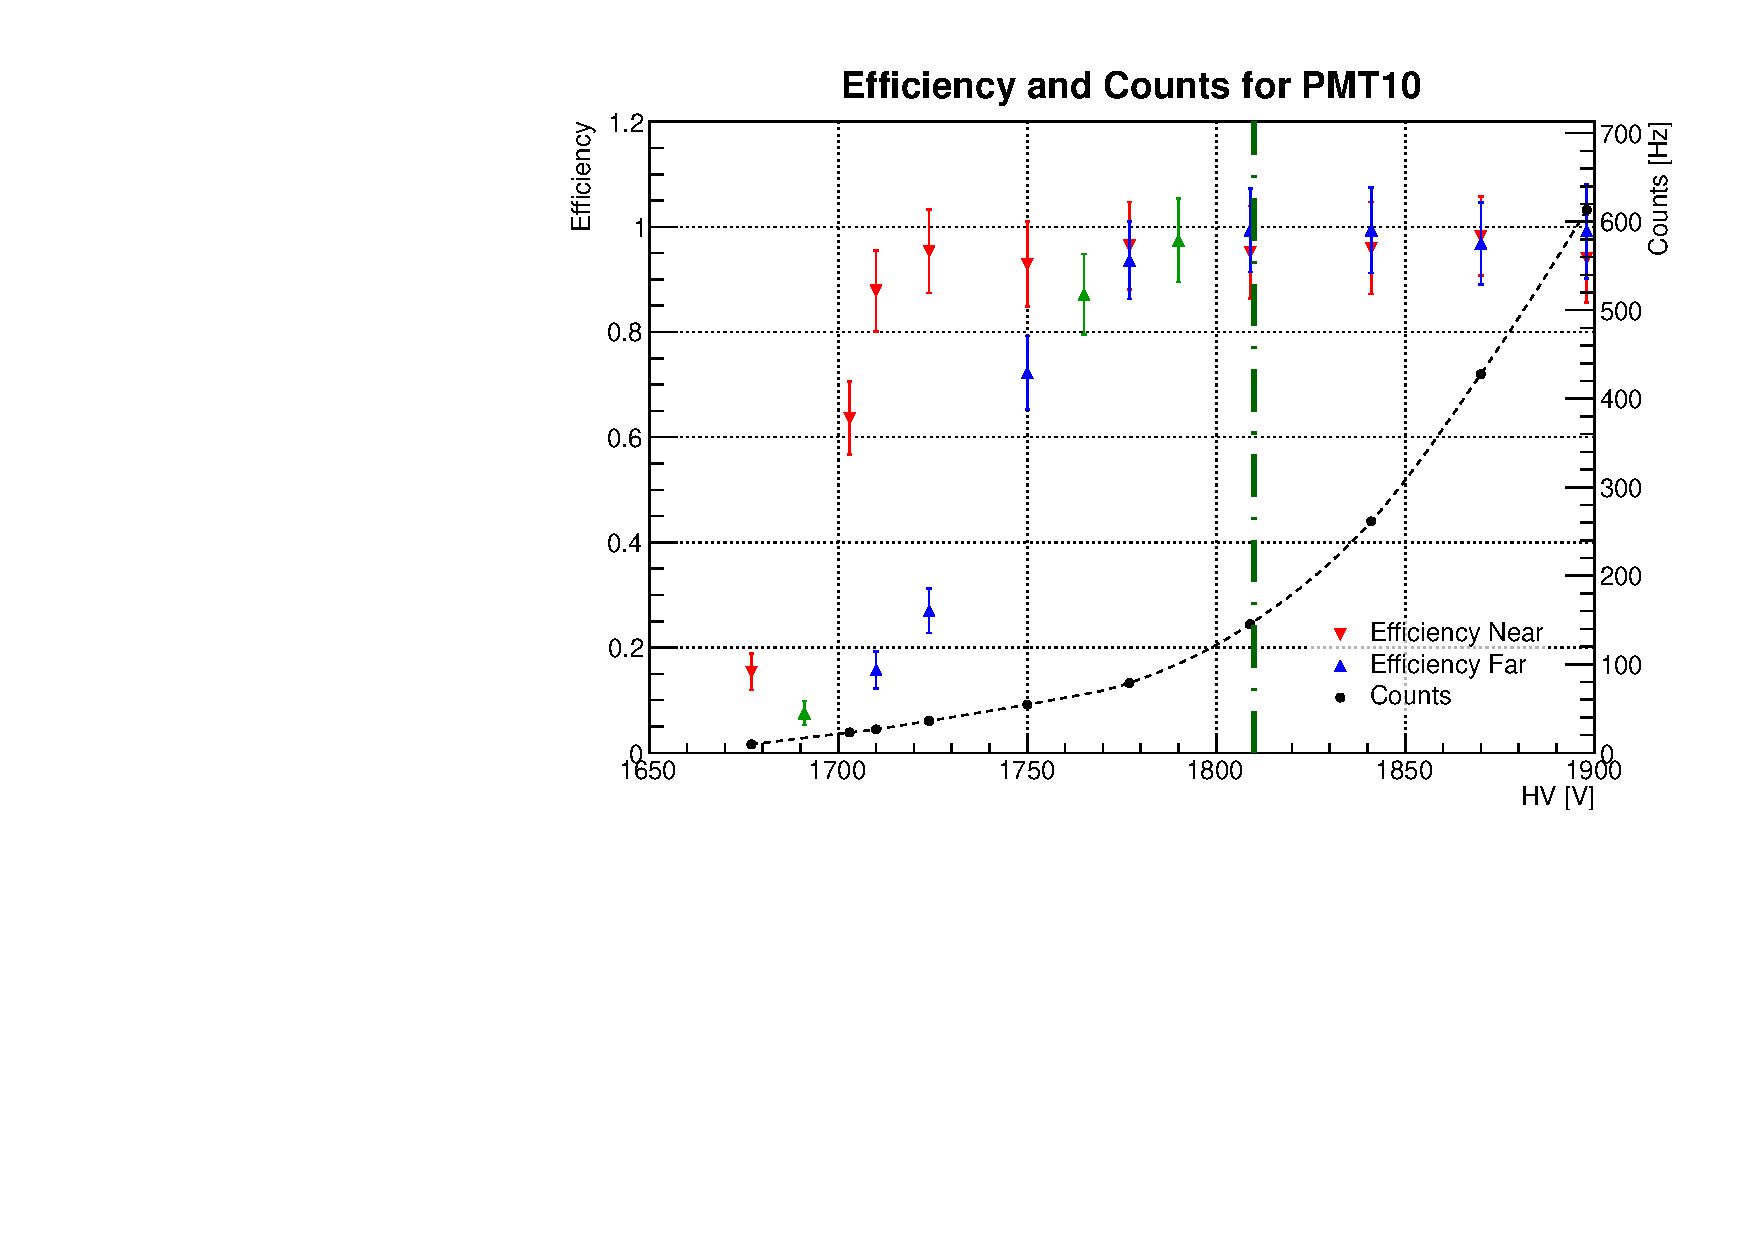
\includegraphics[scale=0.5]{img/eff10.pdf}}}
%	\centerline{
%		\subfloat
%		{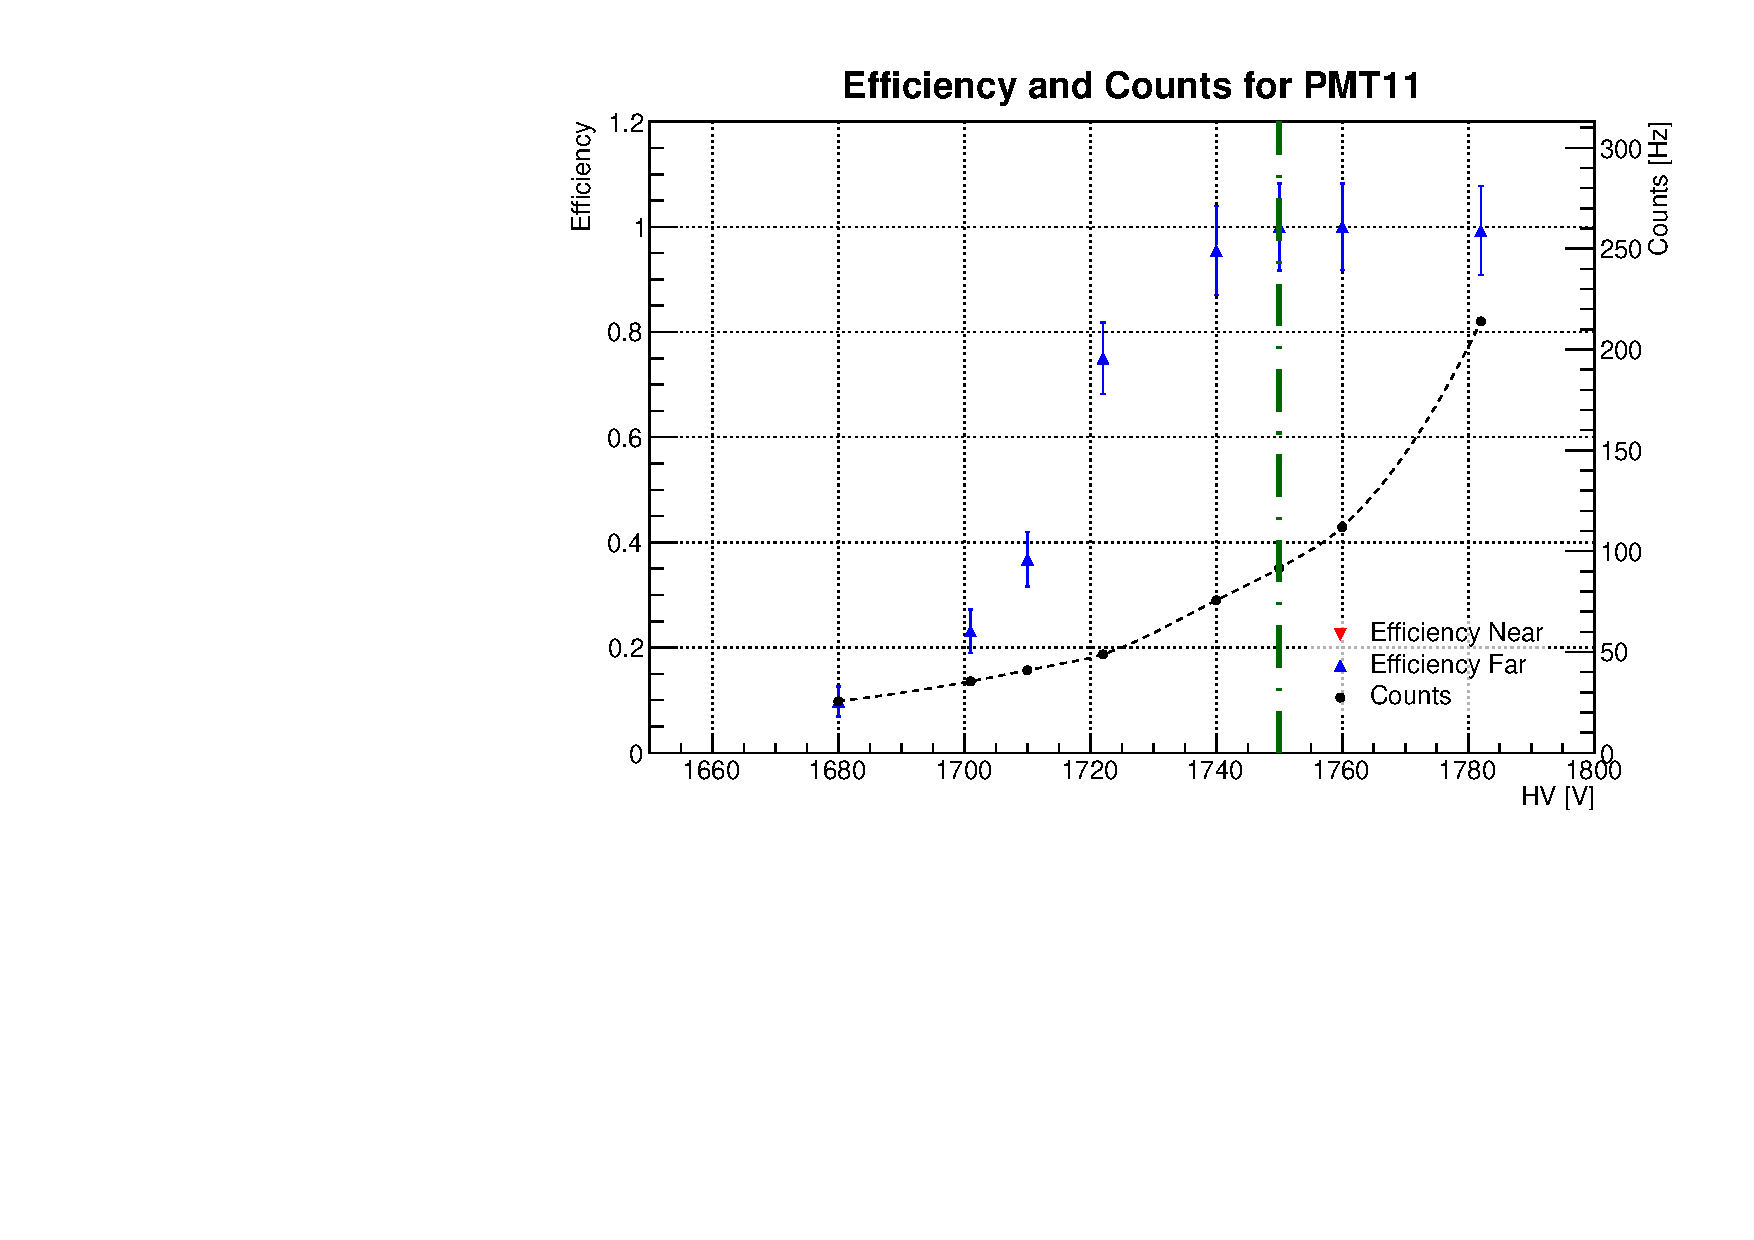
\includegraphics[scale=0.5]{img/eff11.pdf}}
%		\subfloat
%		{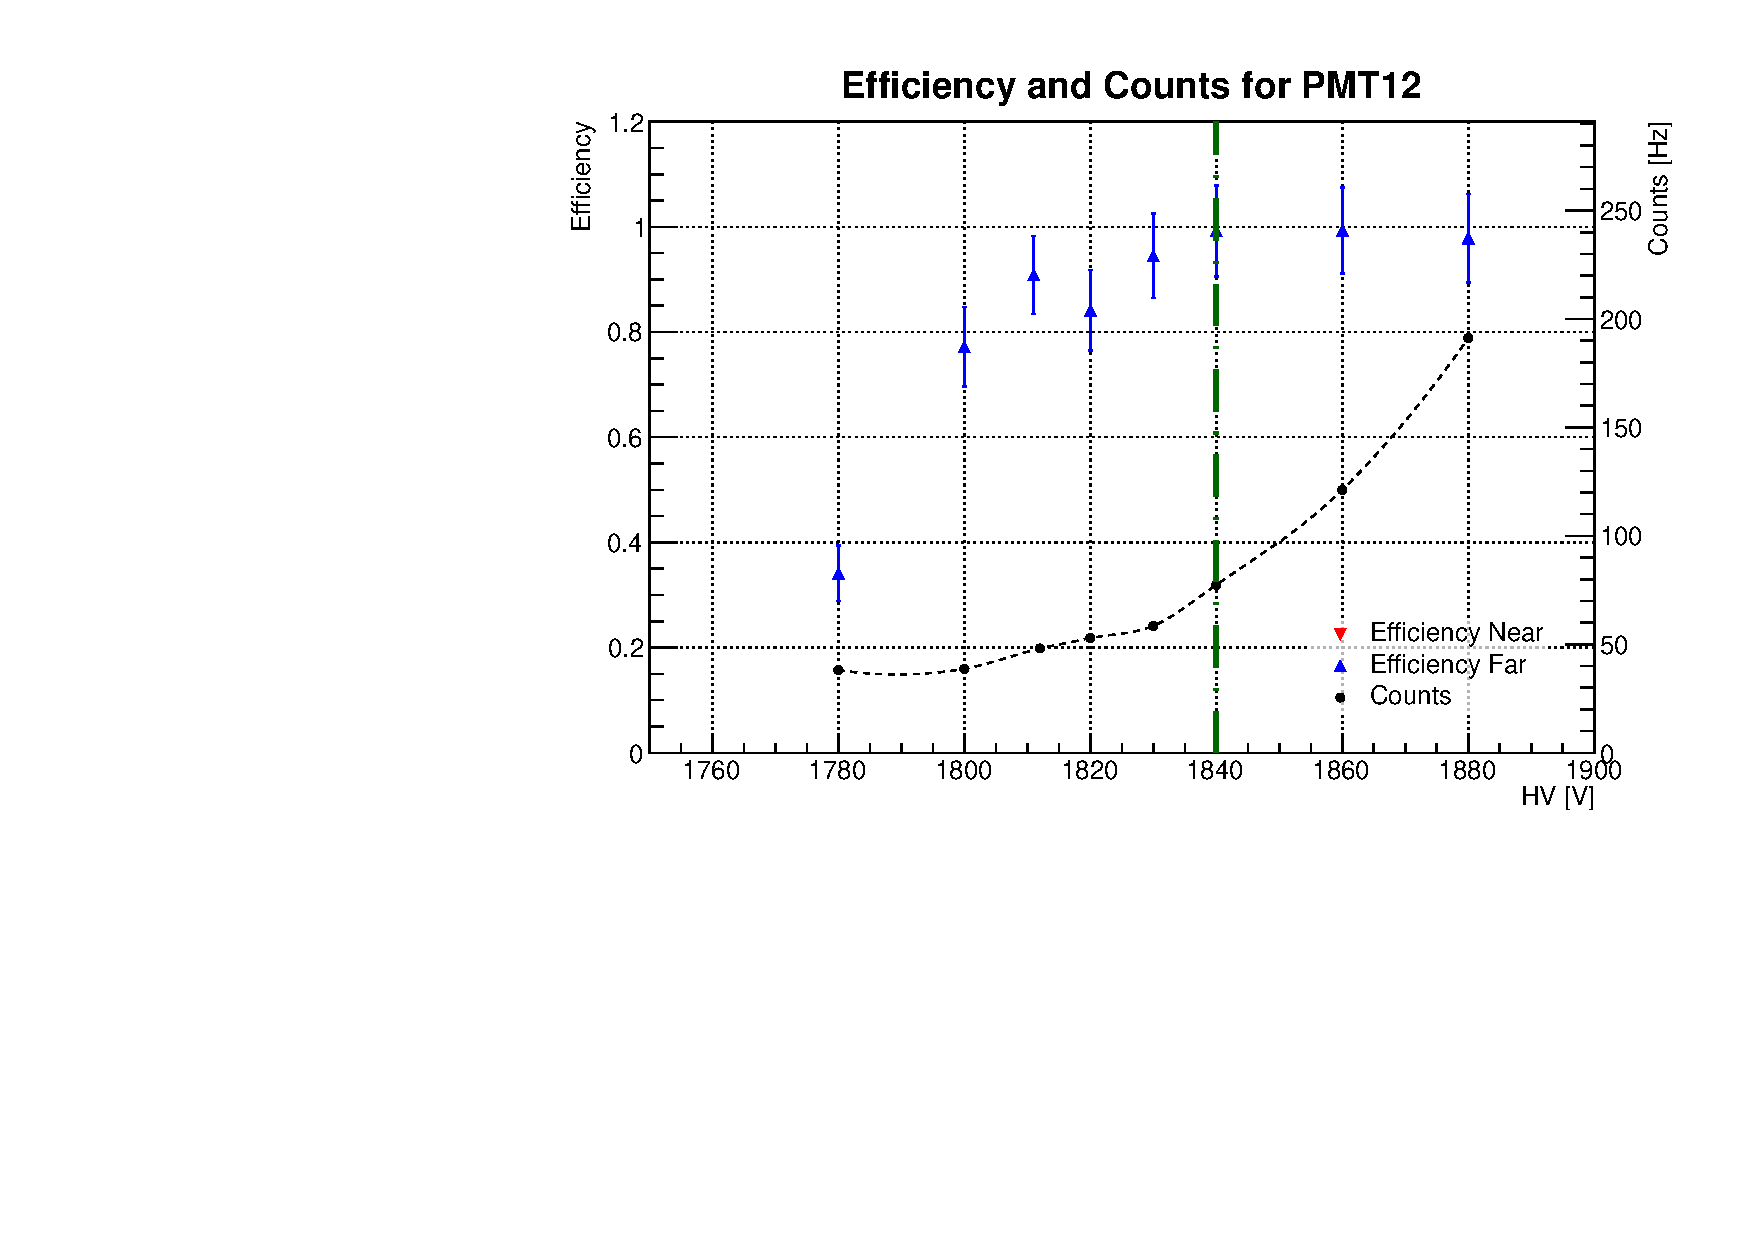
\includegraphics[scale=0.5]{img/eff12.pdf}}}
%\end{figure}
%\begin{figure}[h]
%	\centerline{
%		\subfloat
%		{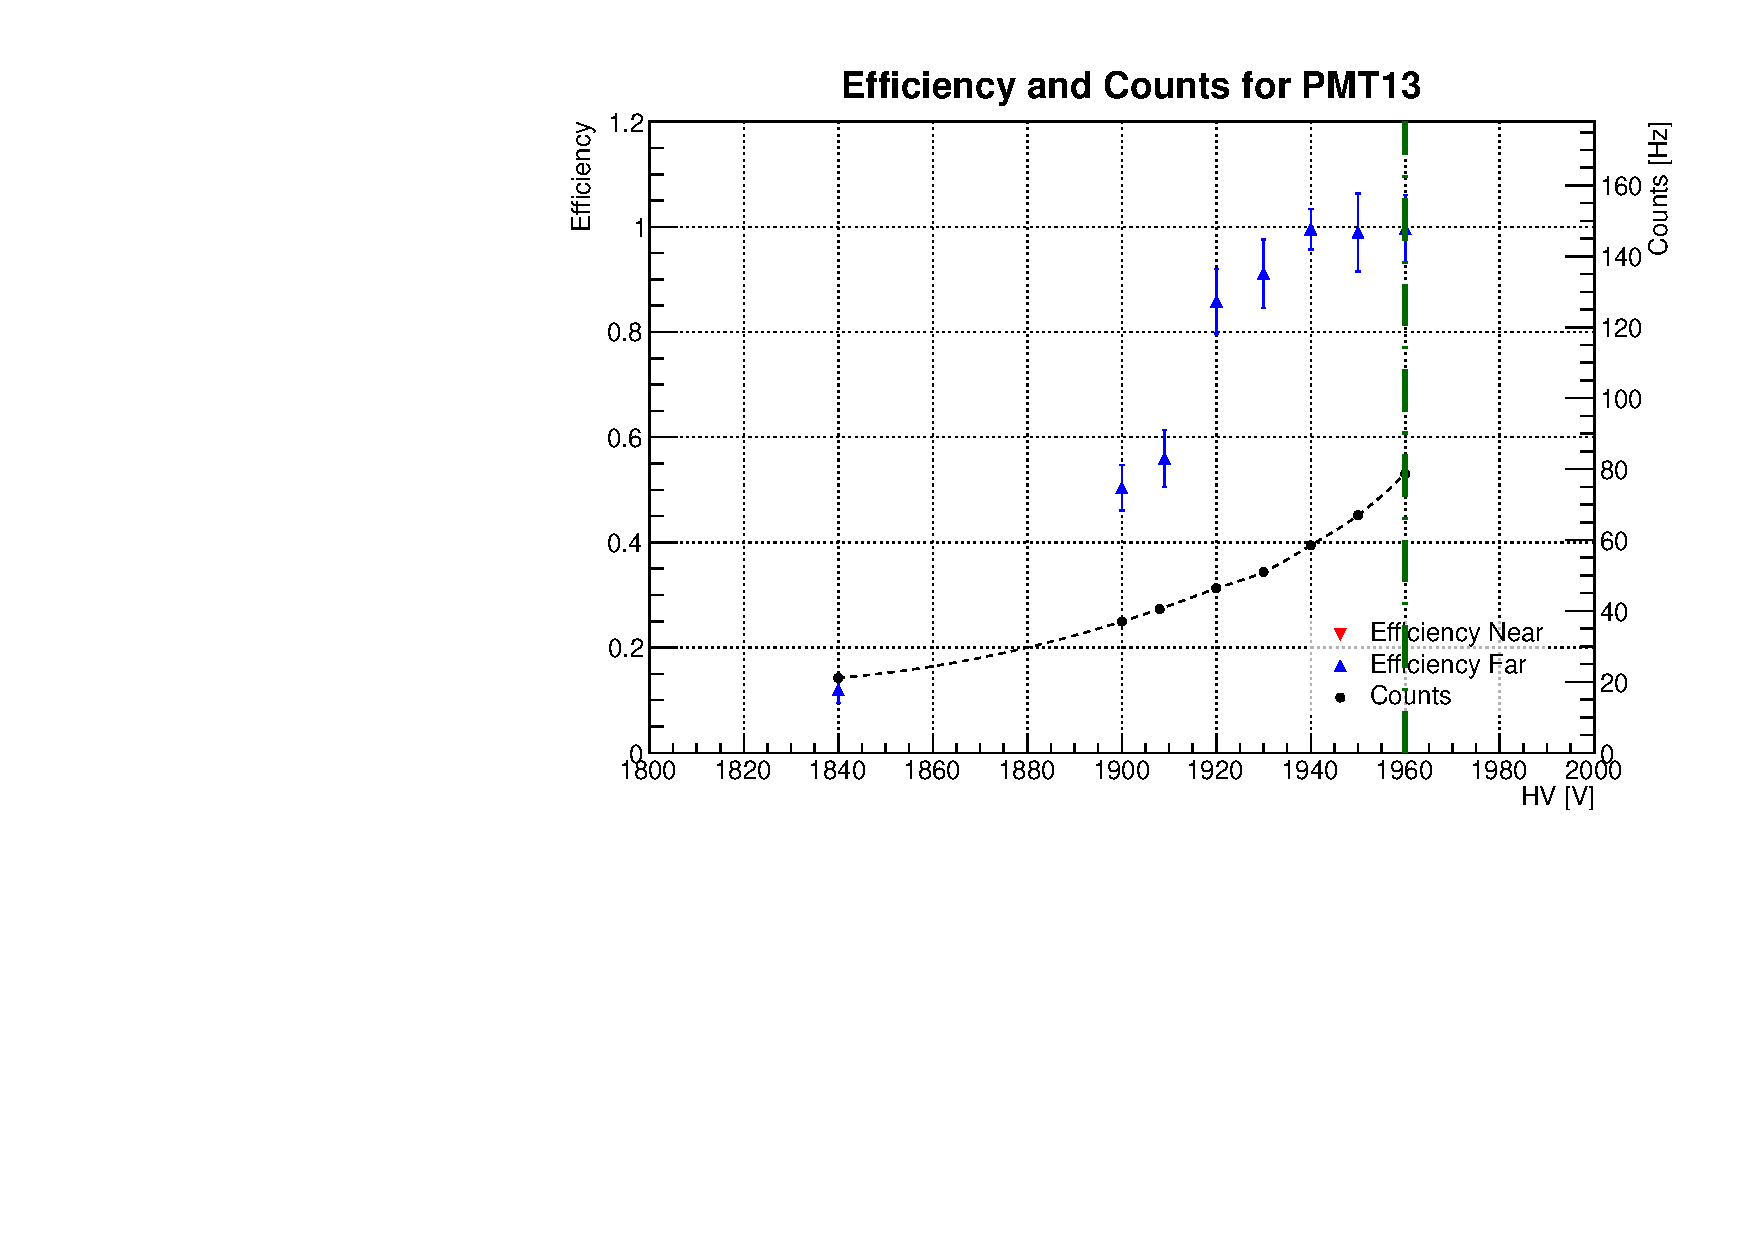
\includegraphics[scale=0.5]{img/eff13.pdf}}
%		\subfloat
%		{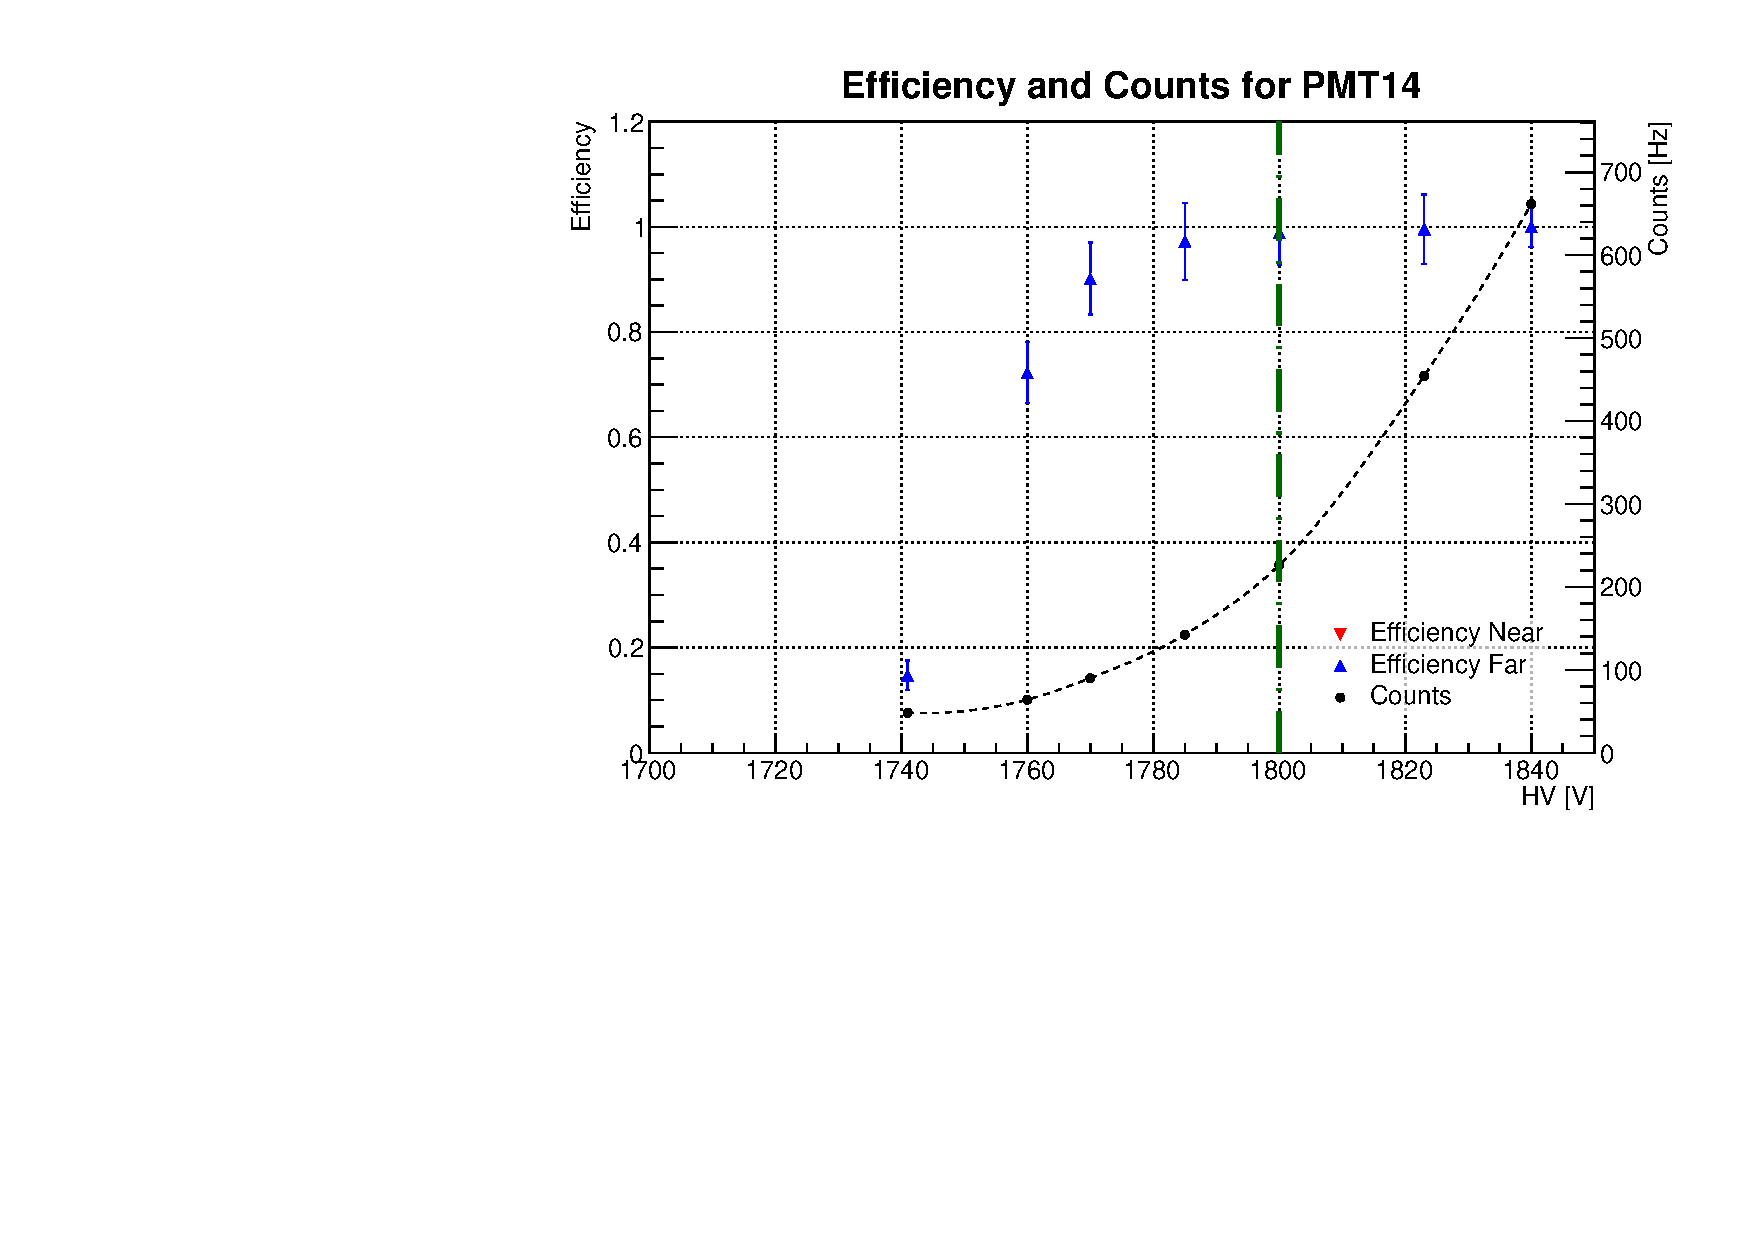
\includegraphics[scale=0.5]{img/eff14.pdf}}}
%\end{figure}

%
\addcontentsline{toc}{section}{\refname}
\begin{thebibliography}{4}
%
\bibitem{pdg2}
K.~A.~Olive et alii, \emph{Particle Data Group}, Chin.~Phys.~C, \textbf{38}, 090001 (2014).
%
\bibitem{pdg}
J. Beringer et alii, \emph{Particle Data Group}, PR \textbf{D86}, 010001 (2012).
%
\bibitem{al} 
A. Grossheim \emph{et al.}, \emph{Decay of negative muons bound in $^{27}$Al}, Phys.~Rev.~, \textbf{D80}, 052012 (2009). 
%
\bibitem{R} R: T.~H. Burnett \emph{et al.}, \emph{Measurement of cosmic-ray muon charge ratio at sea level between energies of 10 and 1500 GeV}, Phys.~Rev.~Lett., \textbf{30}, 937 (1973).
%
\bibitem{pb}
T.~K. Gaisser, \emph{Spectrum of cosmic-ray nucleons, kaon production, and the atmospheric muon charge ratio}, Astropart.~Phys., \textbf{35}, 801-806 (2012).
%
\bibitem{root}
R.~Brun and F.~Rademakers, \emph{ROOT - An Object Oriented Data Analysis Framework, Nucl.~Inst.~Meth.} A 389 (1997) 81.
%
\end{thebibliography}
\end{document}
